\chapter{Current And Voltage Synchronization}
% \stepcounter{chapter}\addcontentsline{toc}{chapter}{Simulation Results}

\section{Introduction}
After extraction of the requirements of the op-amps from the simulink simulations, it is a standard approach to design an ideal system in the cadence environment and cross-verify the functionality as well as the performance of the overall architecture. Then the process of design of the blocks at the transistor level begins. In order to keep the debugging process easier, block-by-block replacement in the ideal architecture, with transistor level blocks is done and the performance is assured with each block replacement. Once the full architecture is transformed from ideal blocks to the transistor level blocks, the blocks are laid-out one by one. A similar technique is exercised and one-by-one the transistor level blocks are replaced by the parasitic extracted blocks until the  complete architecture is laid-out. With post-layout simulation, the performance is insured again. 
%
\begin{figure}[h!]
    \centering
    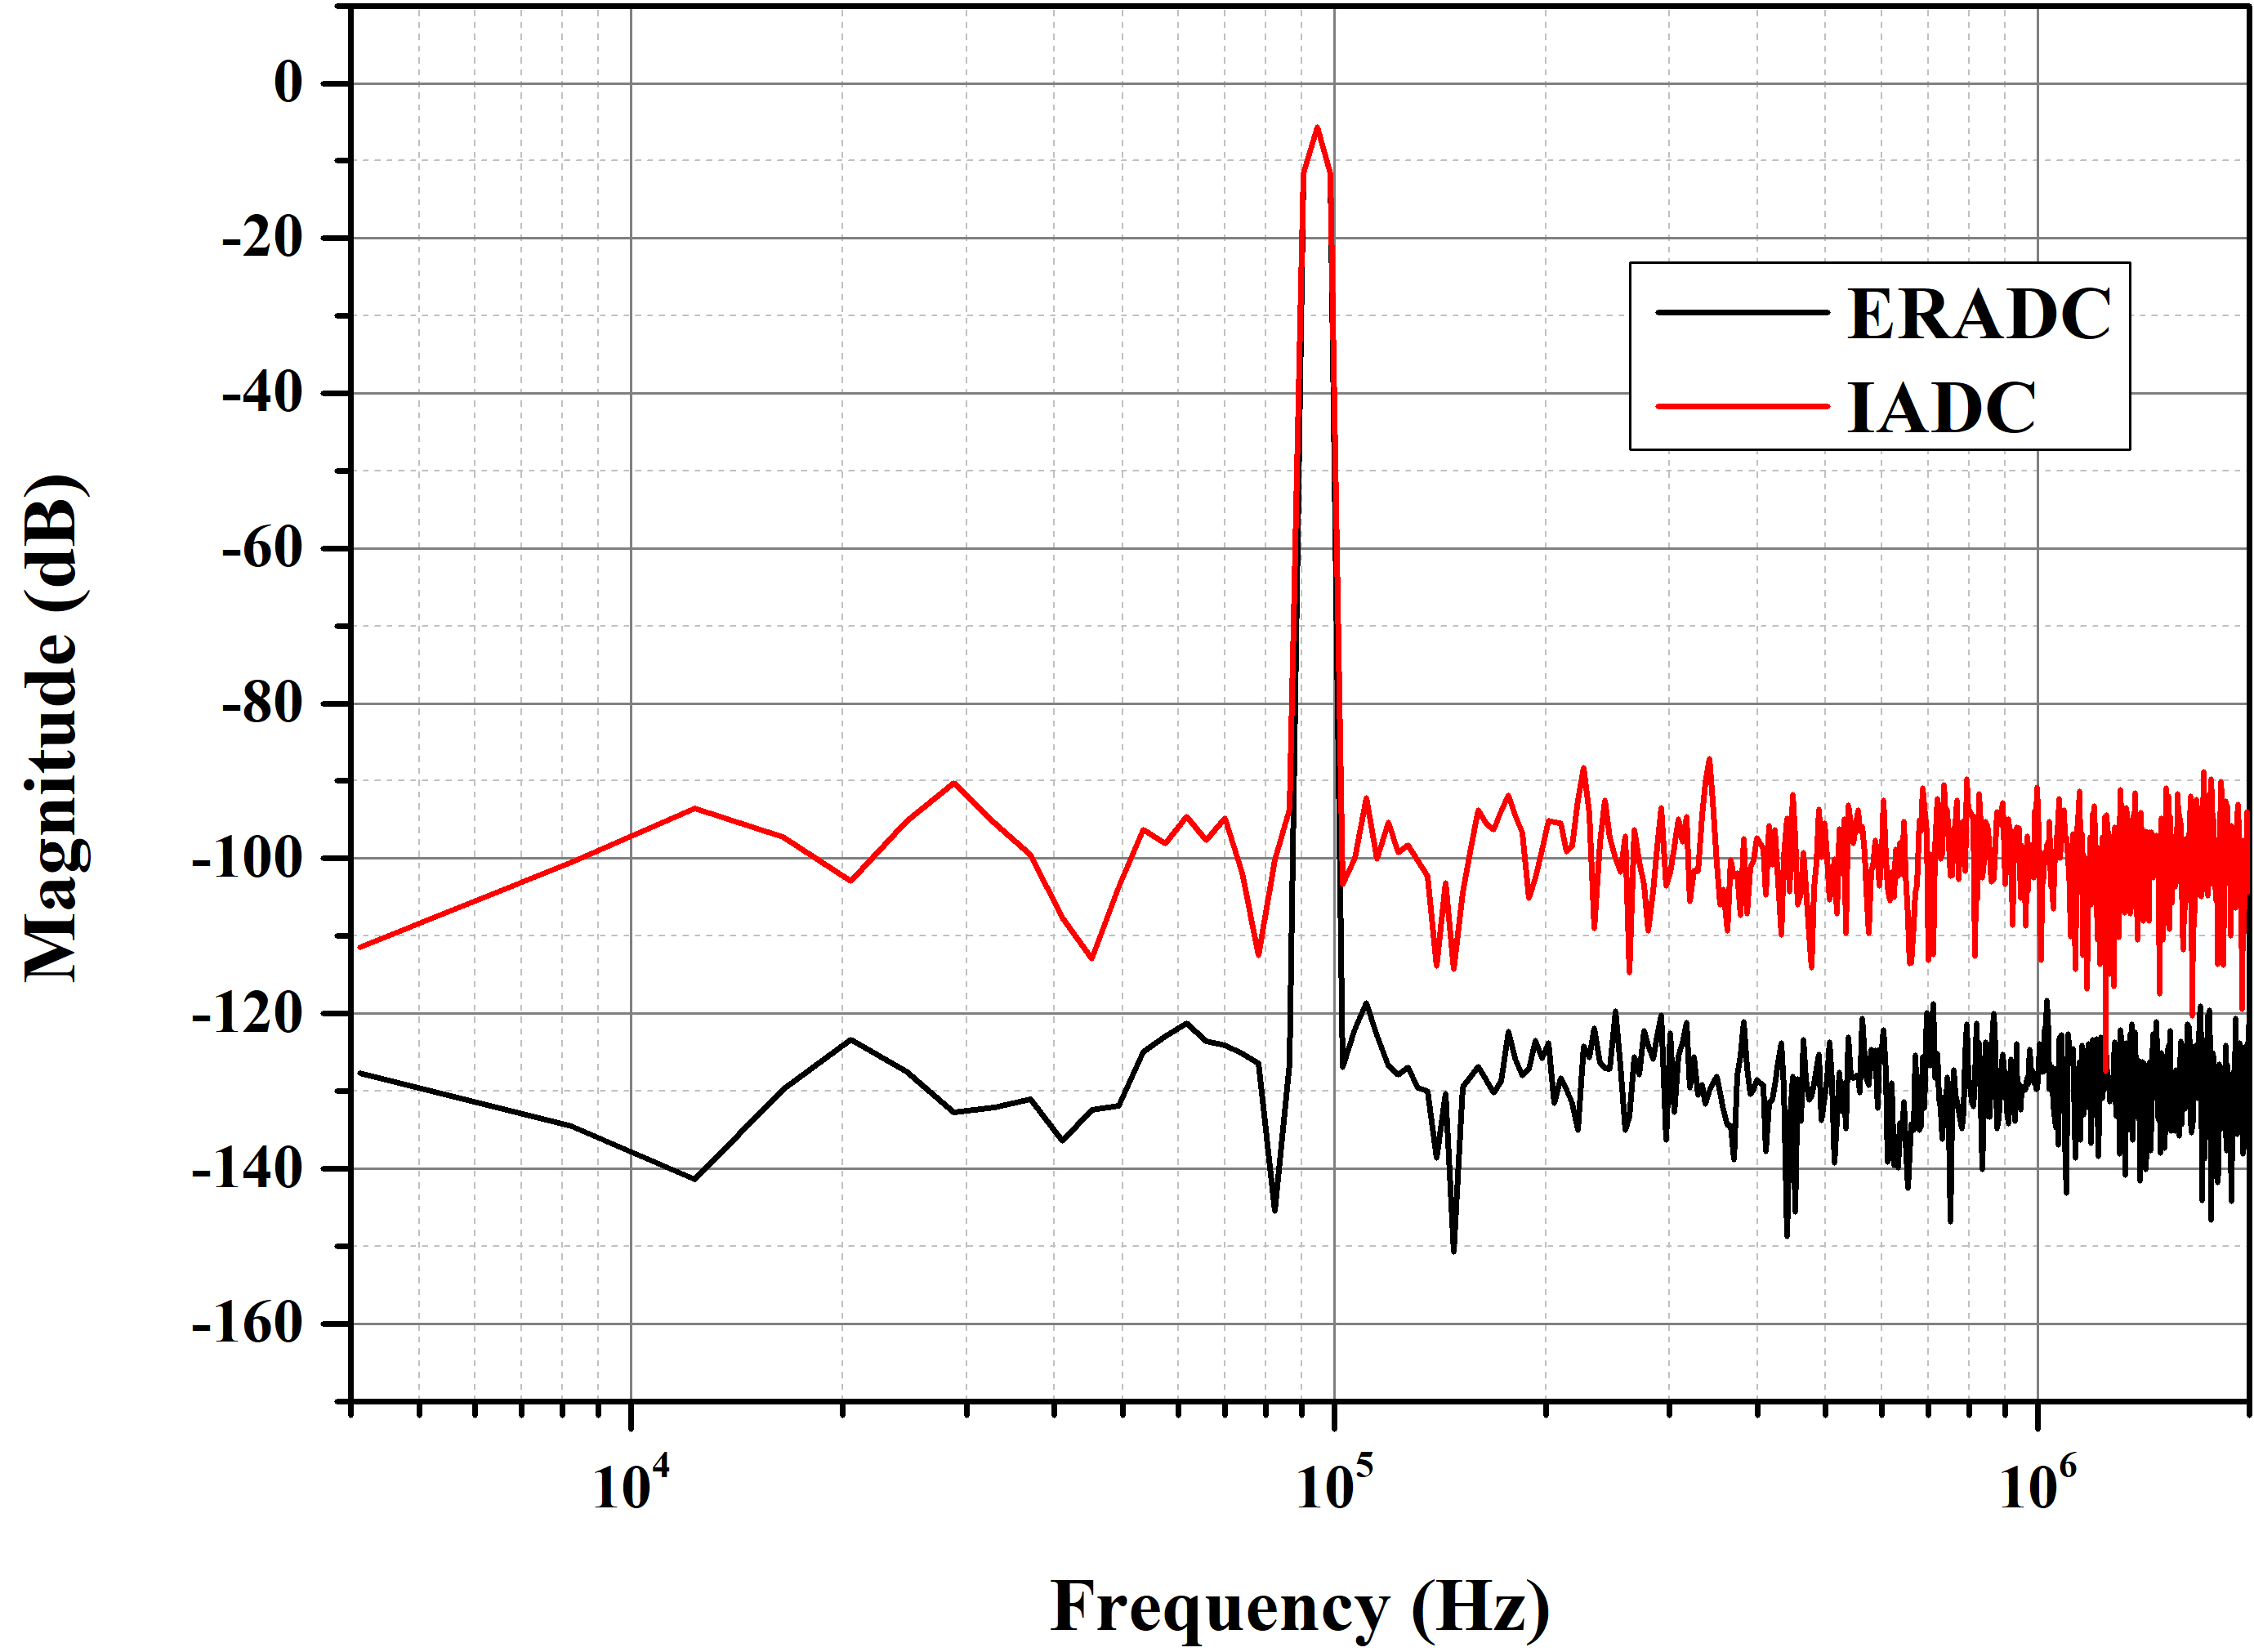
\includegraphics[width=0.8\columnwidth]{Chap06/Figures/PSD_ideal.jpg}
    \caption{Power Spectral Density of the output of Incremental ADC and Extended Range ADC with all the blocks ideal}
    \label{fig:psd_eradc_ideal}
\end{figure}
%

The chapter presents the simulation results in the cadence environment with the three steps described above i.e. with ideal blocks, transistor level blocks of the whole ERADC architecture and post-layout simulation results of the extracted top level. Finally as a maiden version, the first tape-out focuses on the first-stage i.e. Incremental ADC where the characterization of the chip is accomplished with positive results and are presented.
% The ideal architecture of the IADC has been developed in Cadence environment using a second order structure with 3-bit quantizer and 5-bit ADC in the extended counting.

% %
% \begin{figure}
%     \centering
%     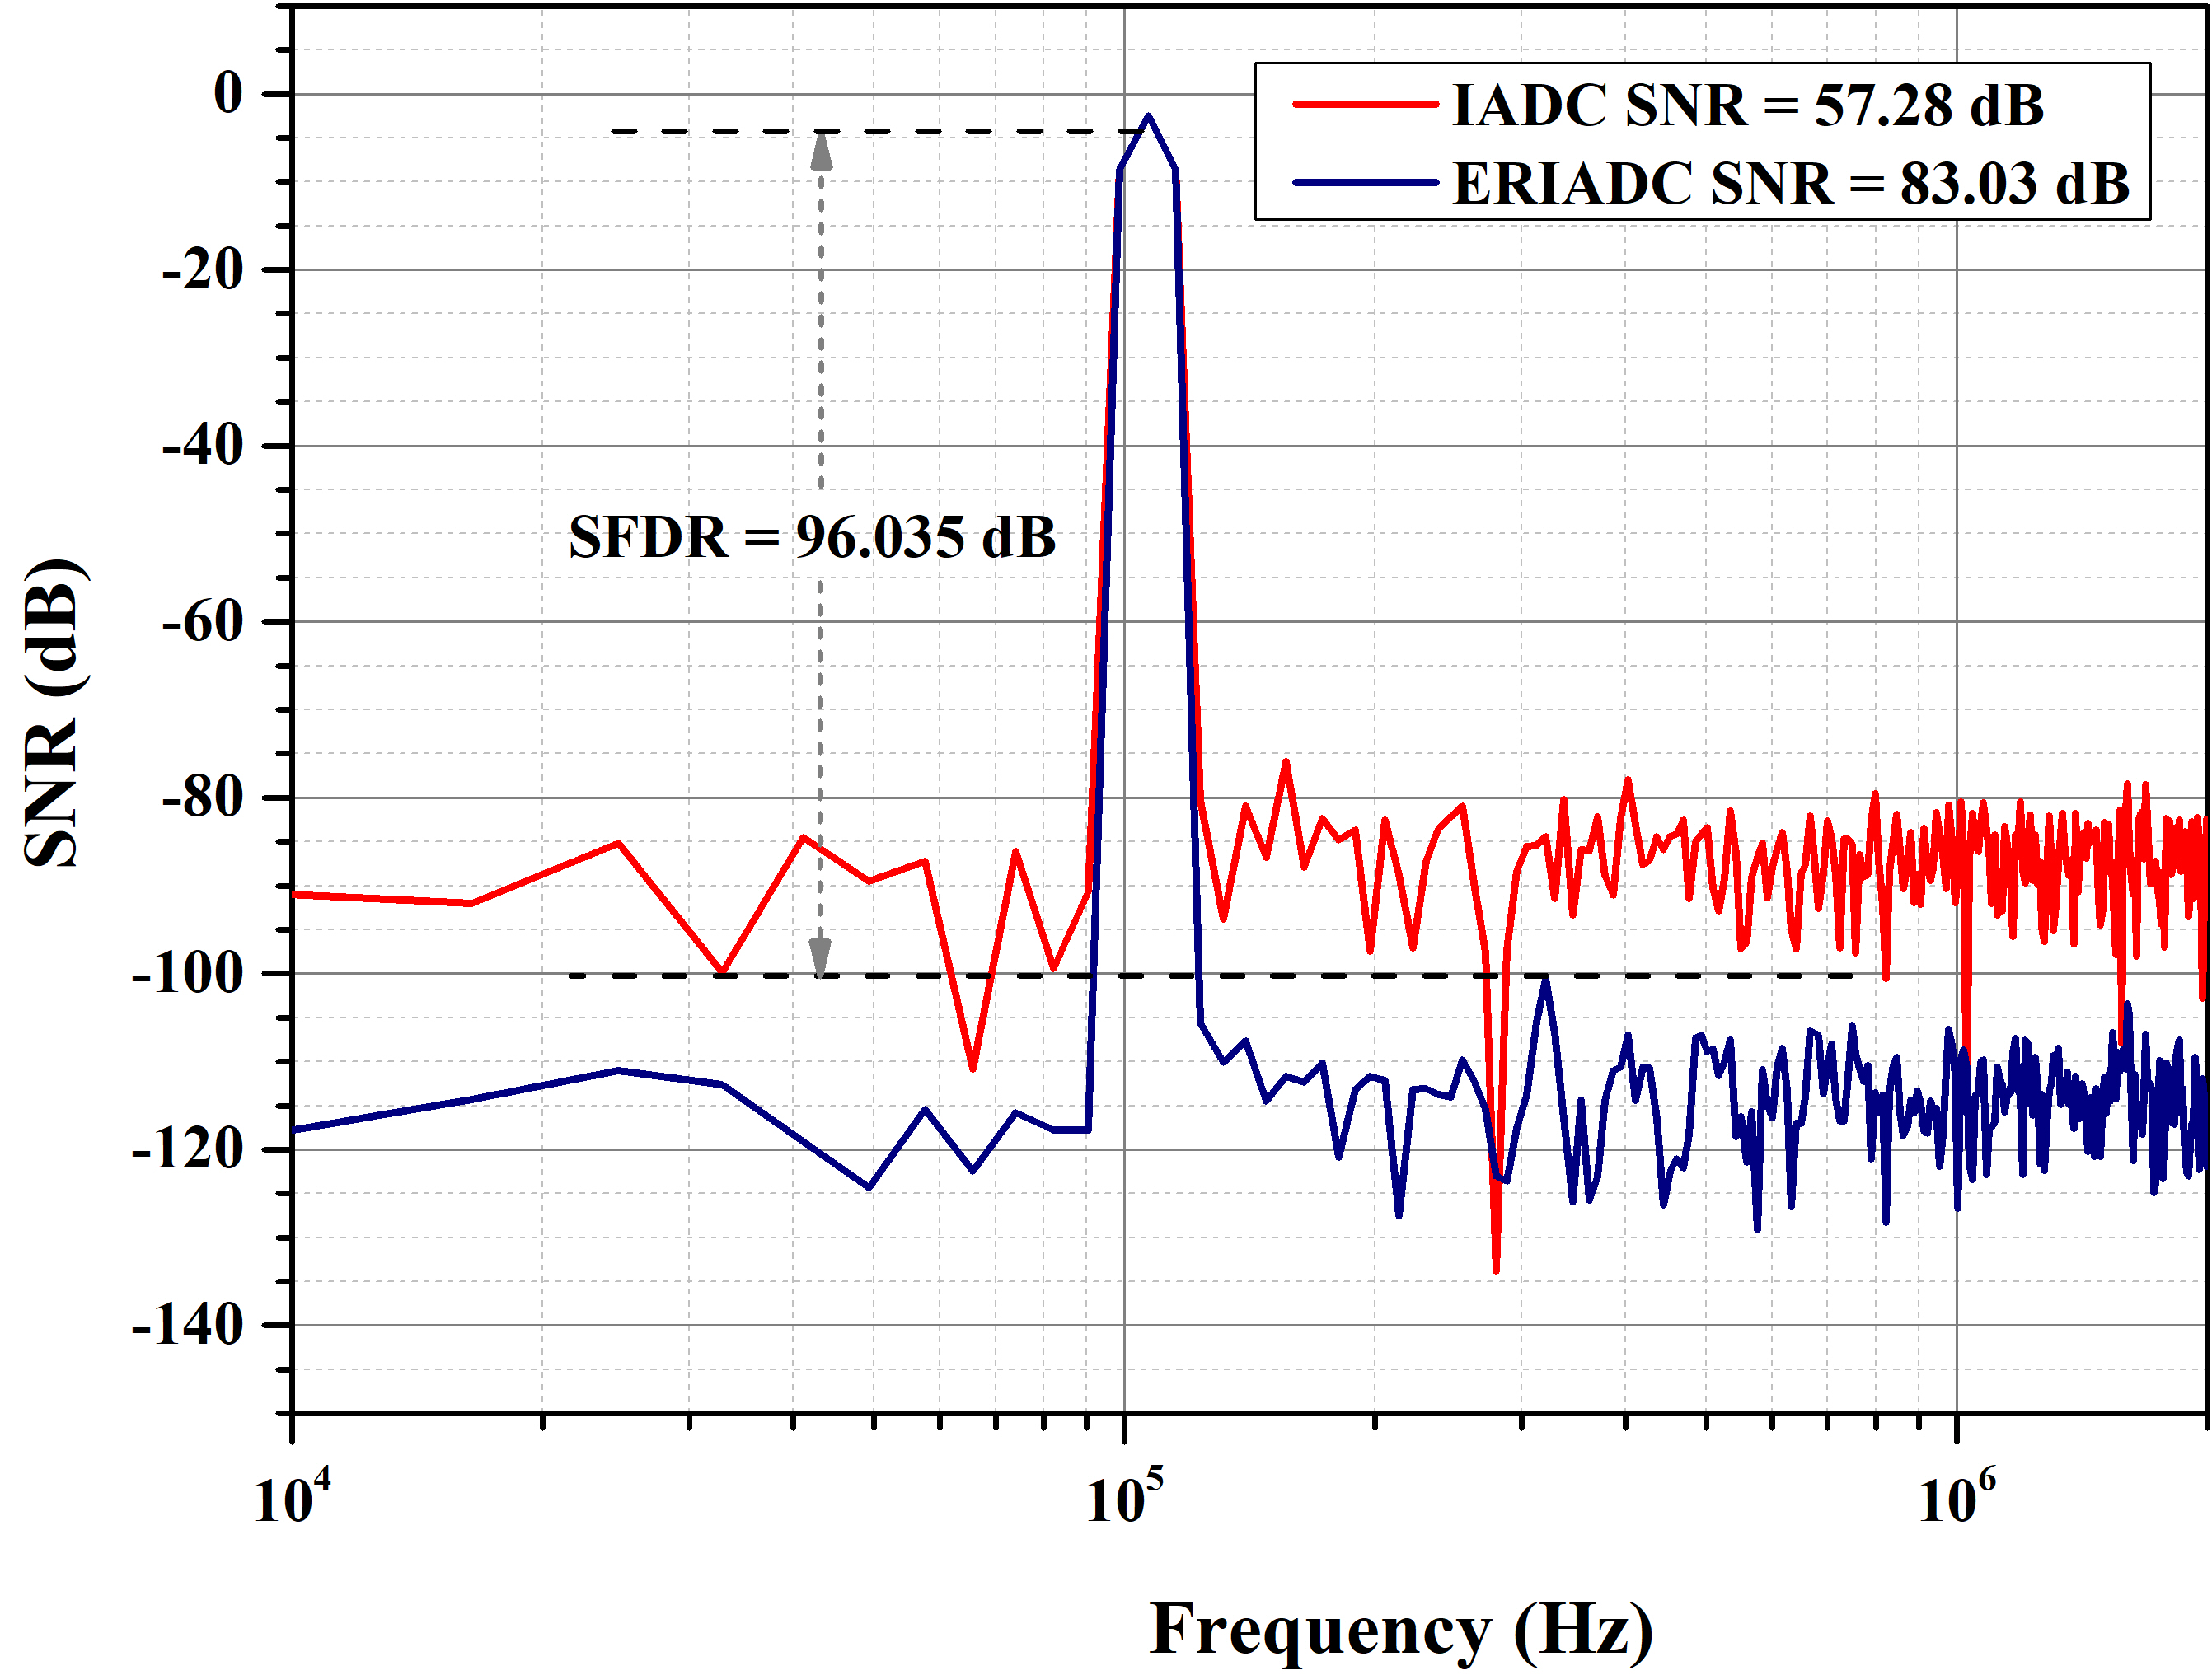
\includegraphics[width=\columnwidth]{Chap06/Figures/PSD_ERADC1.jpg}
%     \caption{Caption1}
%     \label{fig:my_label1}
% \end{figure}
% %


% \begin{figure}[h]
%     \centering
%     \subfigure[]
%     {
%         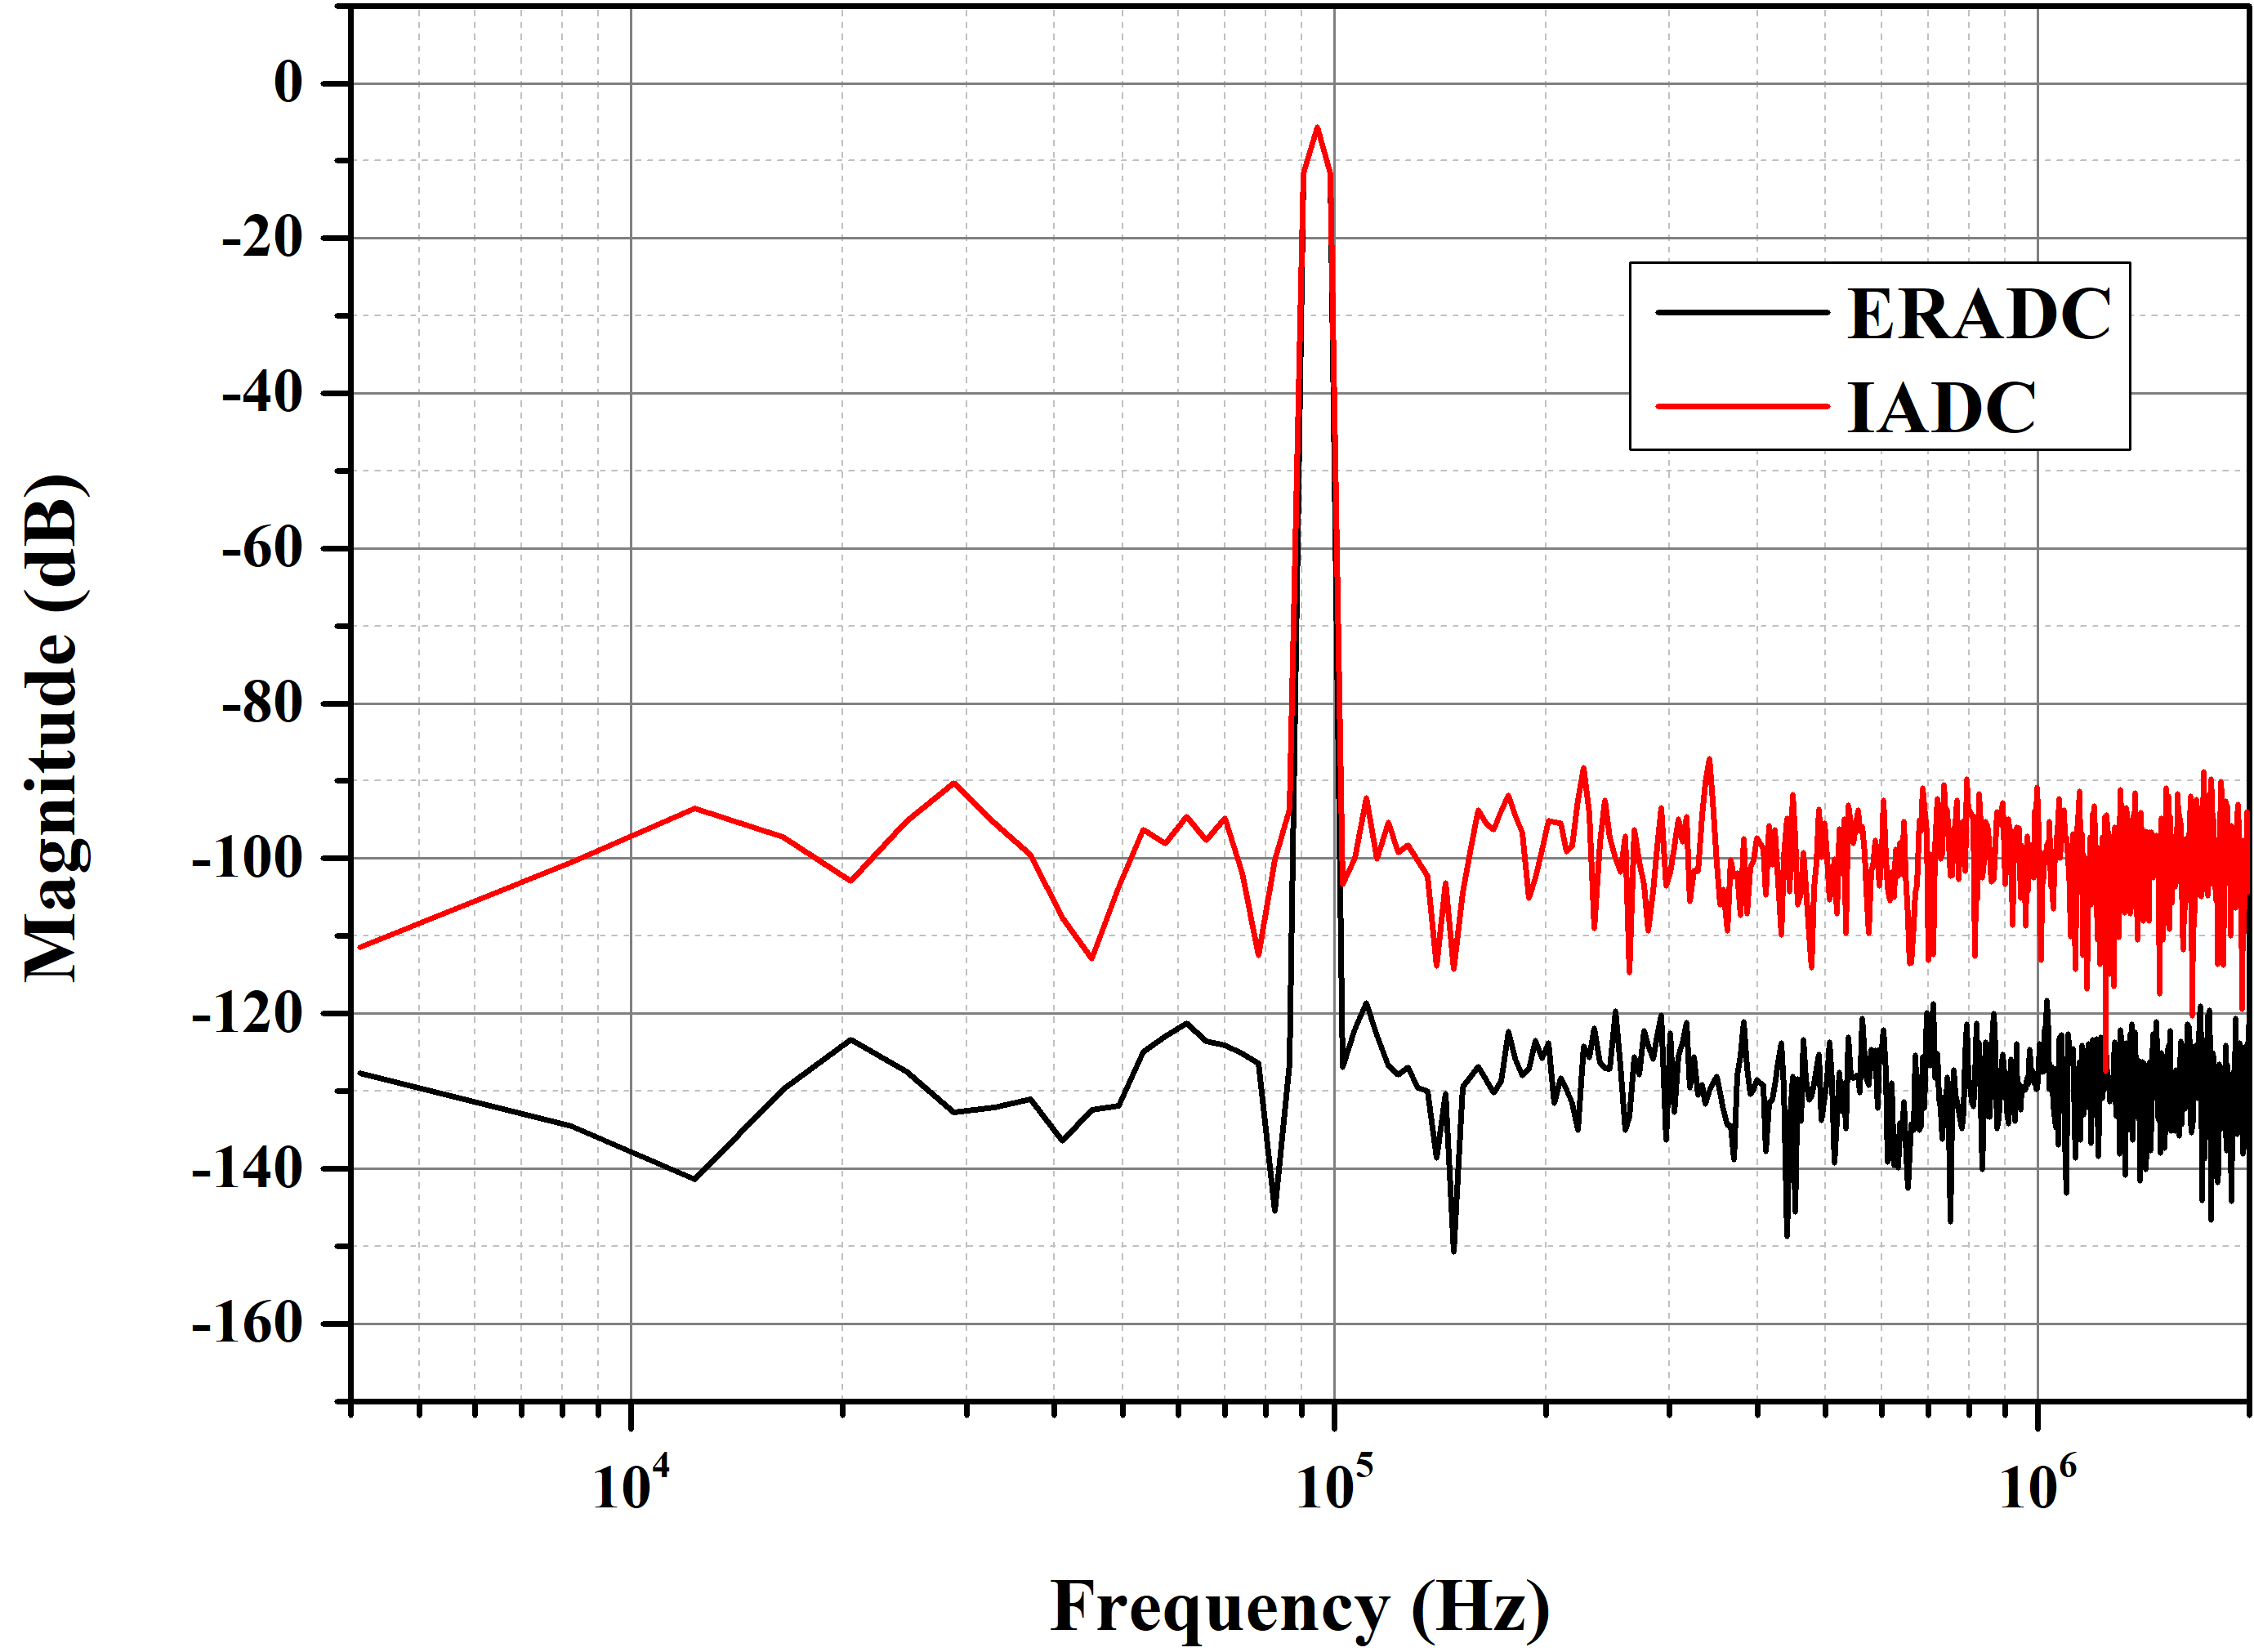
\includegraphics[scale=.28]{Chap06/Figures/PSD_ideal.jpg}
%     }
%     \\
%     \subfigure[]
%     {
%         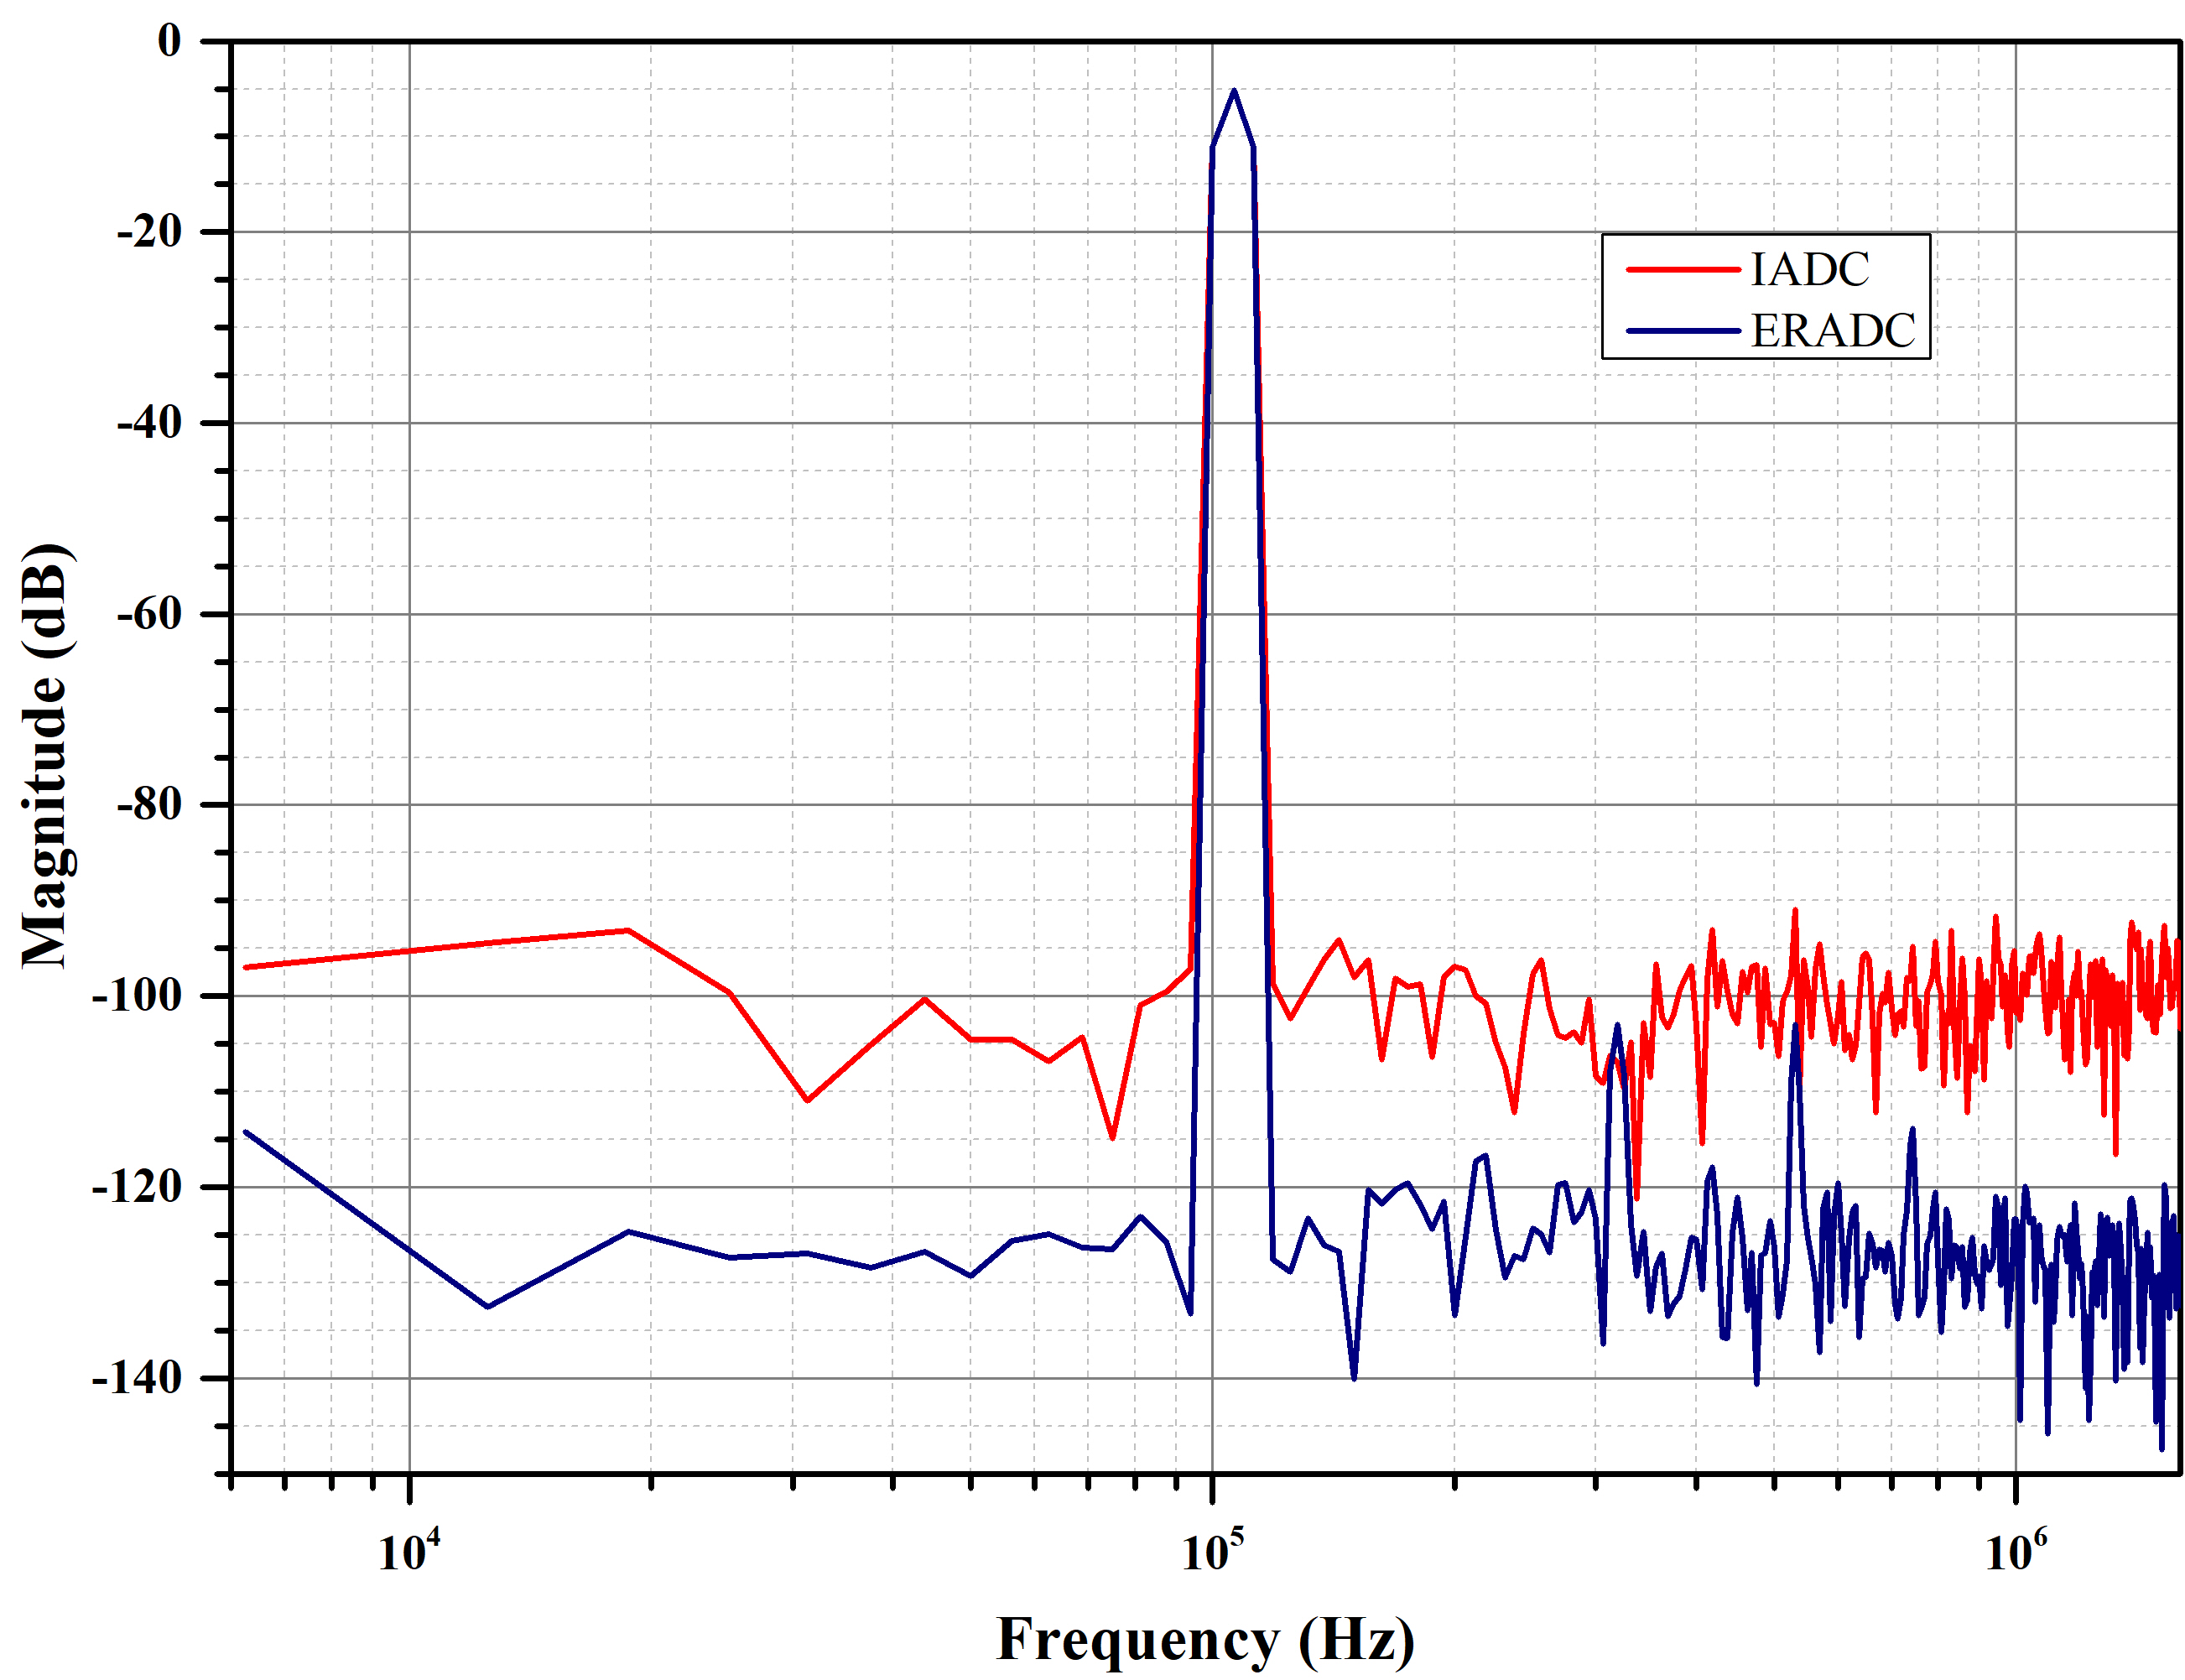
\includegraphics[scale=.28]{Chap06/Figures/PSD_sch.jpg}
%     }
%     \qquad
%     \subfigure[]
%     {
%         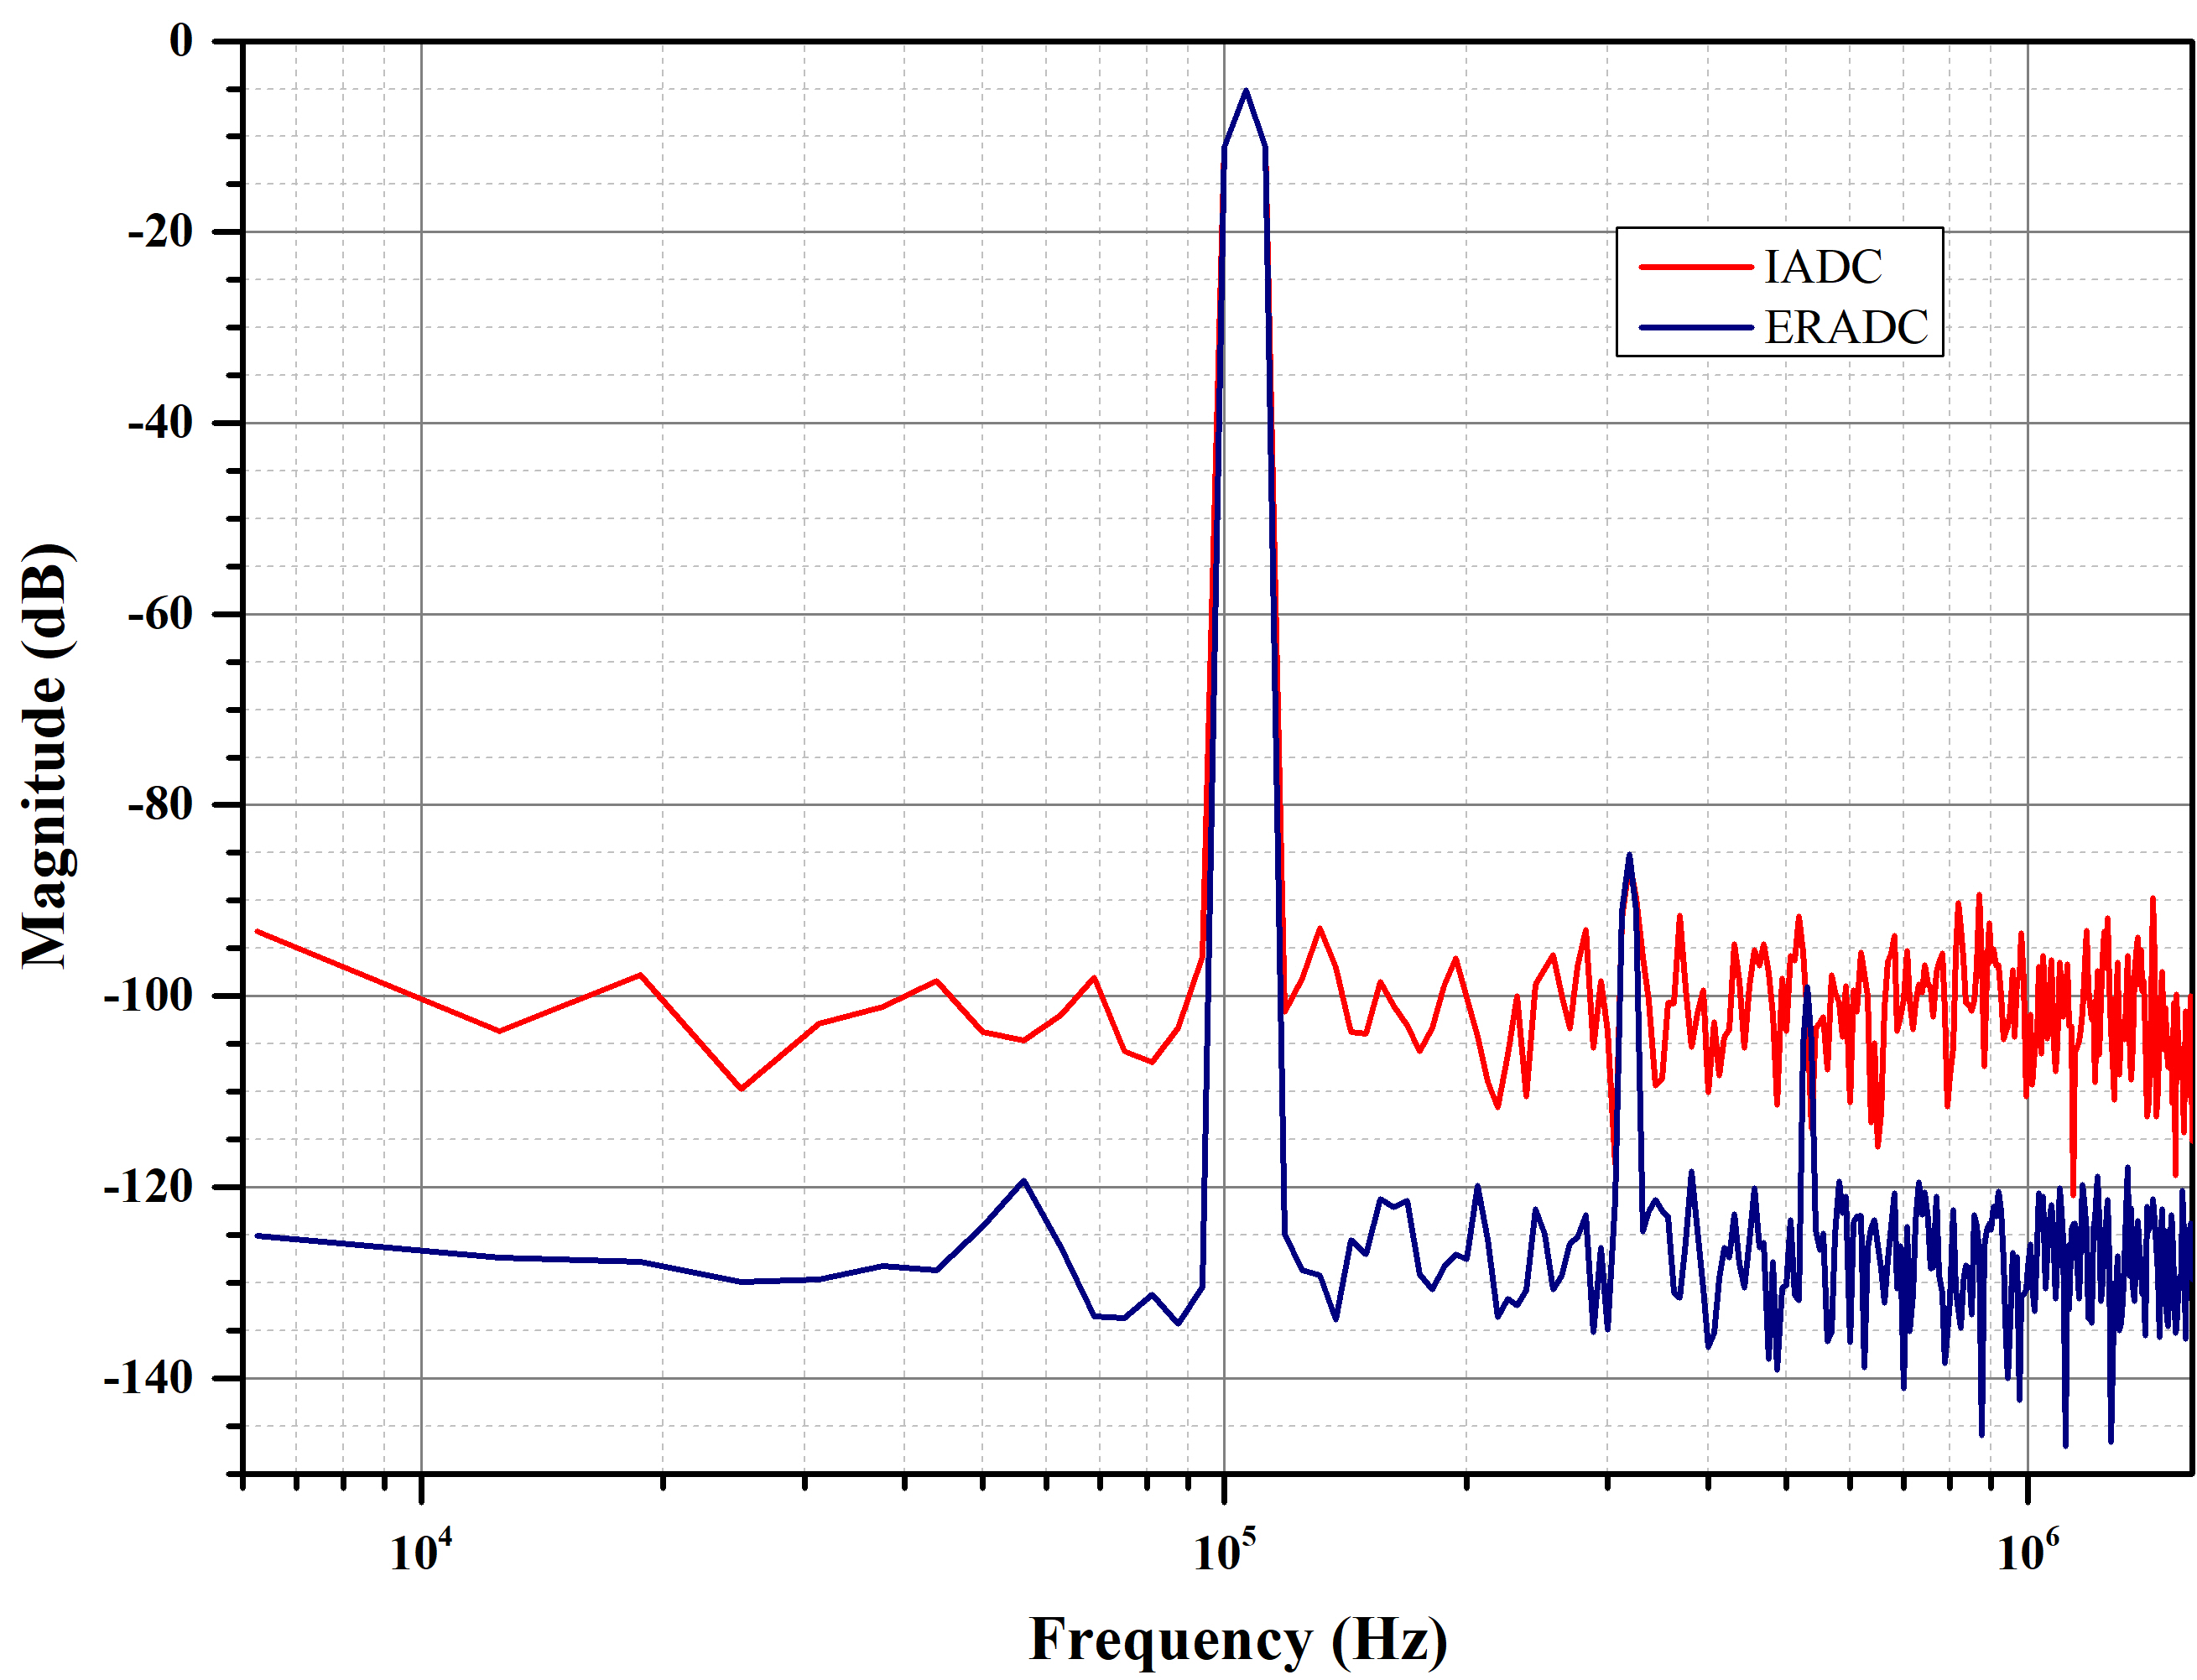
\includegraphics[scale=.28]{Chap06/Figures/PSD_ISDM_av.jpg}
%     }
%     \caption
%     {
%         PSD of the Extended Range Incremental ADC with (a) all the ideal blocks
%         (b) Transistor level blocks
%         (c) Extracted Simulation
%     }
%     \label{PSD}
% \end{figure}
% \begin{figure}[h]
% \centering
% \includegraphics[width=0.5\columnwidth]{}
% \caption{Power Spectral Density of the output of Incremental SDM and Extended Range ISDM with all the blocks ideal}
% \label{PSD_ERISDM_IDEAL}
% \end{figure}
% \begin{figure}[h]
% \centering
% \includegraphics[width=0.5\columnwidth]{}
% \caption{Power Spectral Density of the output of Incremental SDM and Extended Range ISDM at Transistor Level}
% \label{PSD_ERISDM_SCH}
% \end{figure}
% \begin{figure}[h]
% \centering
% \includegraphics[width=0.5\columnwidth]{}
% \caption{Post-Layout simulation Power Spectral Density of the Incremental SDM}
% \label{PSD_ISDM_AV}
% \end{figure}
\section{Simulation Results}
% For second order modulator, with OSR value of 18, the expected ideal value of the SNR of the IADC is 60~dB while that with residual ADC is 86~dB, as shown in Fig. \ref{PSD}(a). When simulated at the schematic level, non-idealities of the blocks brings the overall SNR down to 83.7 dB (Fig. \ref{PSD}(b)). The post-layout simulation result is shown in the Fig. \ref{PSD}(c) where along with non-idealities, the parasitics also plays role, the SNDR of the IADC, however, stays at the same level.


The simulated output spectra of the IADC and of the ERADC are shown in Fig.~\ref{fig:psd_eradc_ideal}\ref{fig:psd_eradc_sch} and \ref{fig:psd_iadc_sav}. The input signal is a sinusoid with an amplitude of -6~dB with respect to full-scale at frequency of 100~kHz while the architecture is clocked at a frequency of 80~MHz. 
%
\begin{figure}[h!]
    \centering
    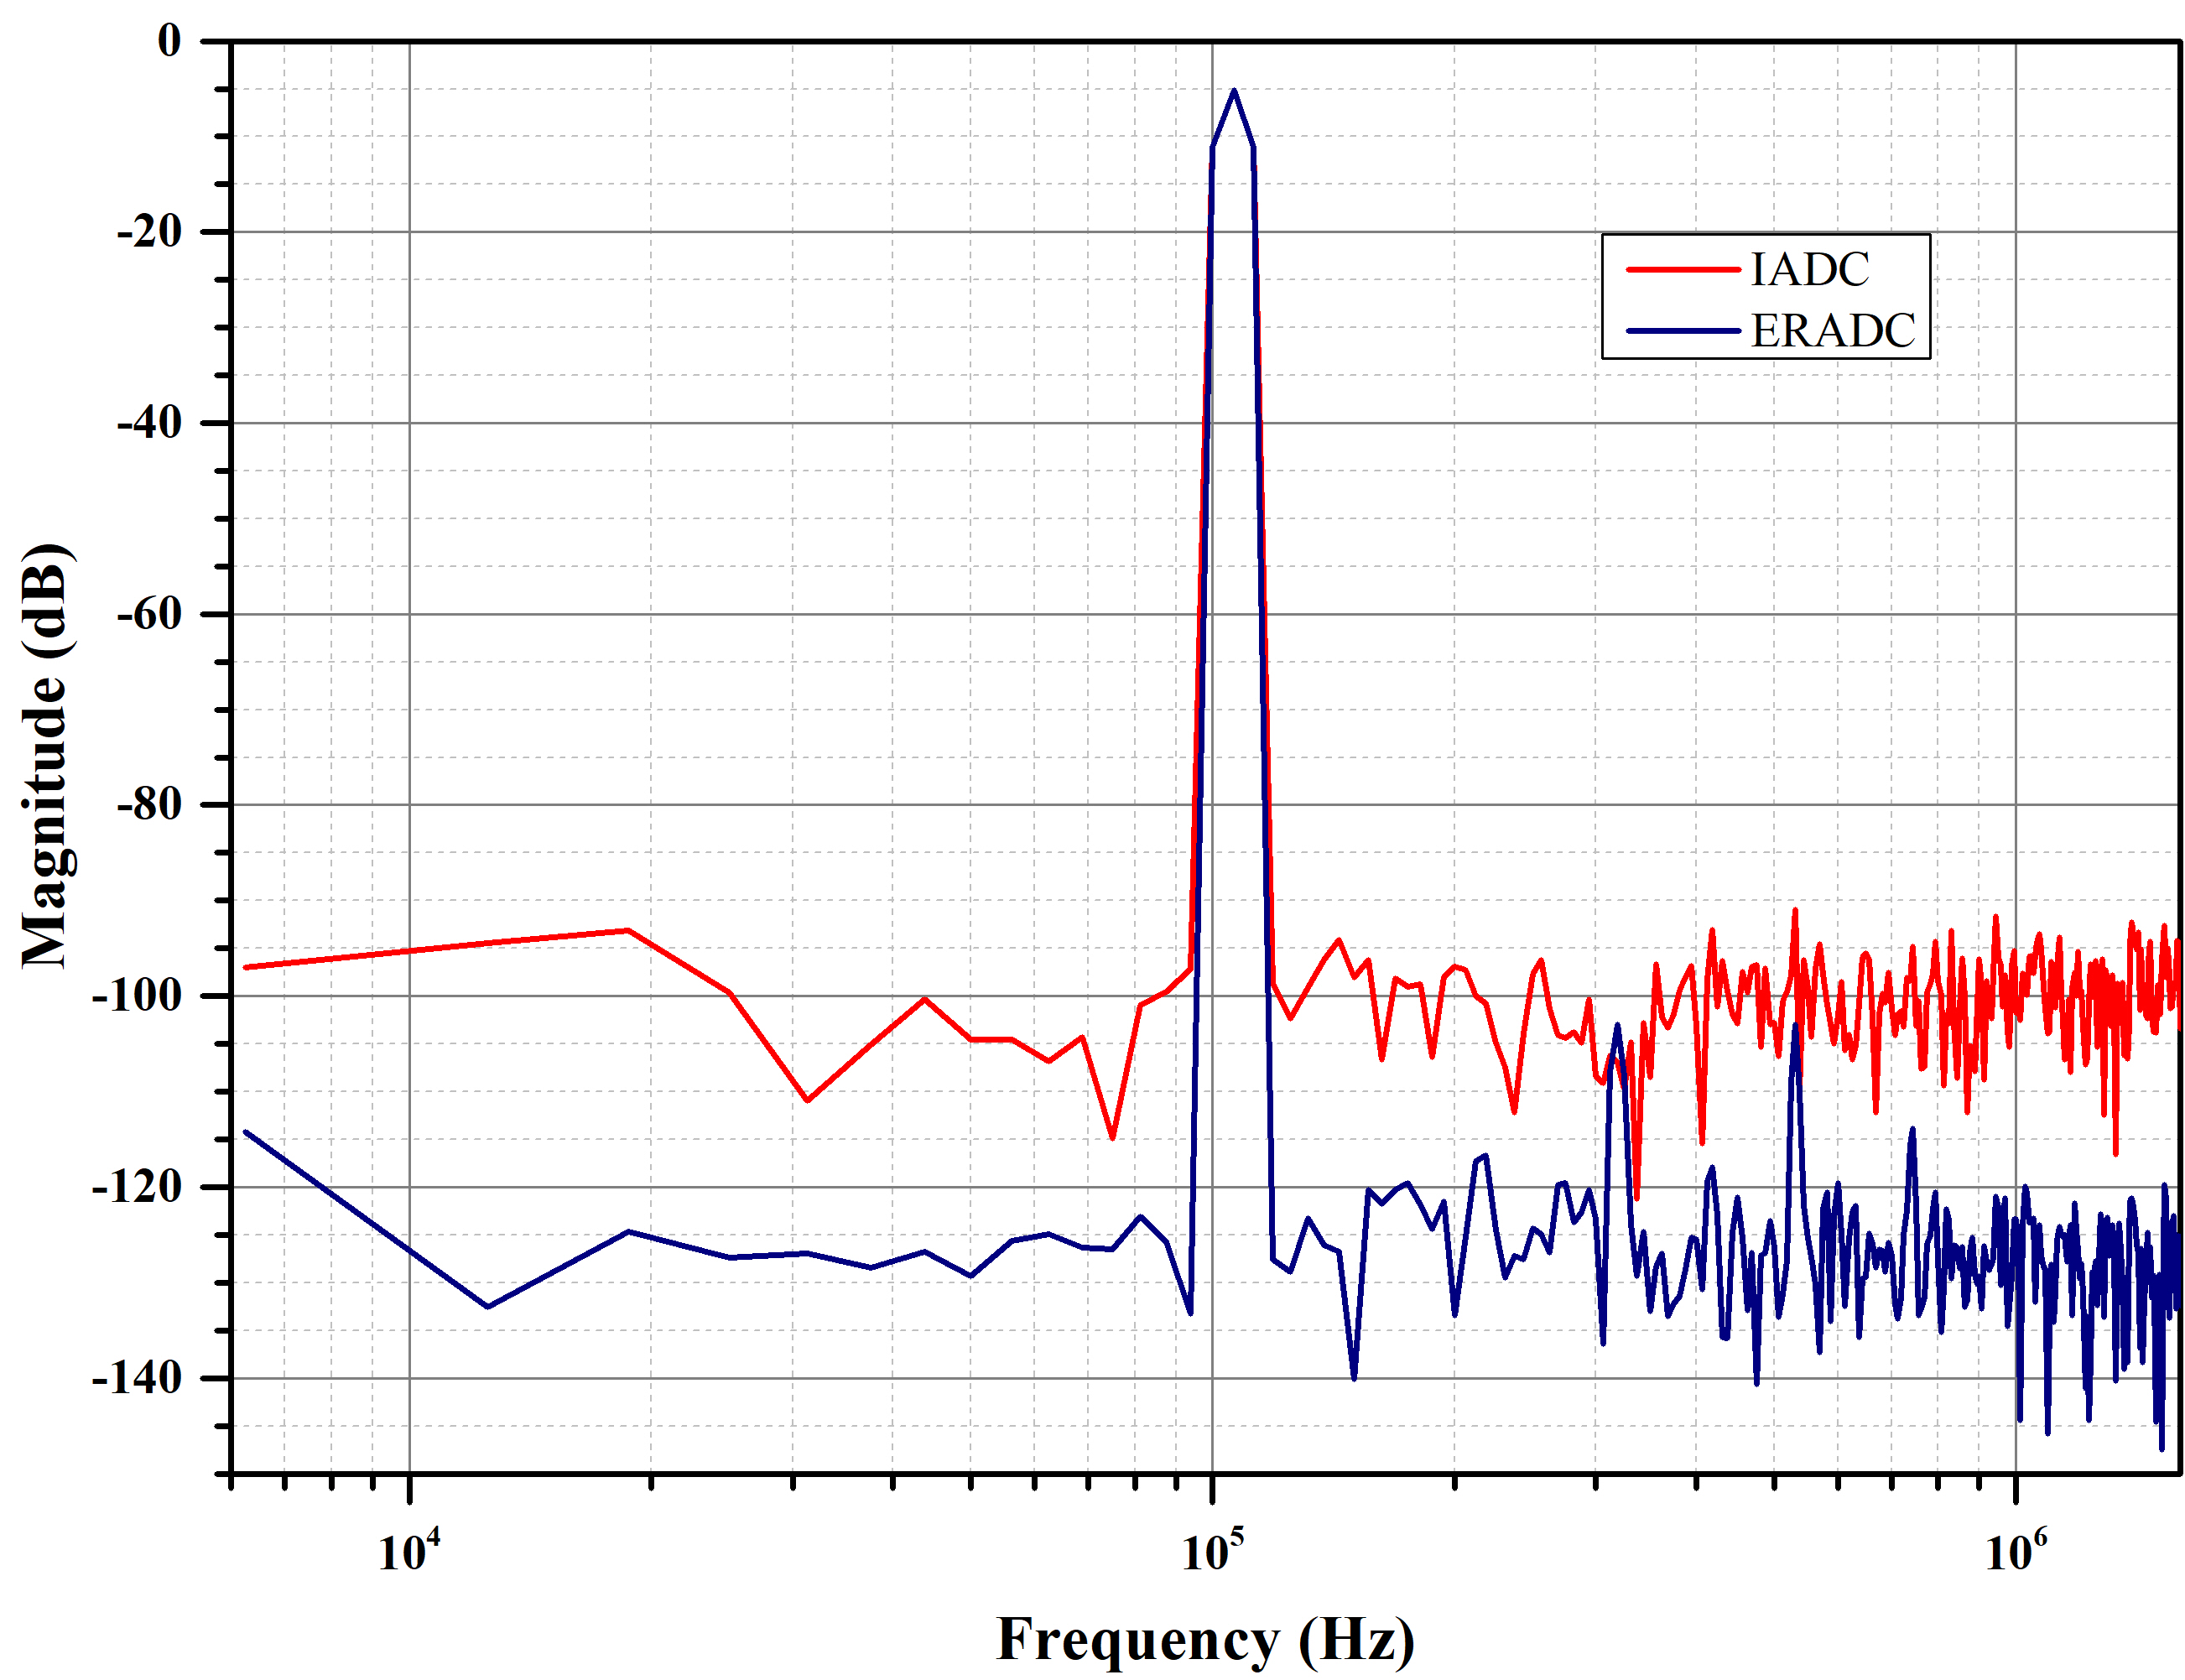
\includegraphics[width=0.8\columnwidth]{Chap06/Figures/PSD_sch.jpg}
    \caption{Power Spectral Density of the output of Incremental SDM and Extended Range ISDM at Transistor Level}
    \label{fig:psd_eradc_sch}
\end{figure}
%

In case of ERADC architecture with ideal blocks, the SNR that can be achieved from the coarse quantization is around 60~dB with a noise floor around -100~dB. However, the overall SNR delivered after the recombination of the coarse and fine quantization is 86.86~dB, i.~e. 26~dB better than the IADC standalone, and the noise floor is as low as -125~dB. The overall Spurious-Free Dynamic Range (SFDR) achieved is around 96~dB as shown in Fig.~\ref{fig:psd_eradc_ideal}.

The simulations results of the ERADC architecture with transistor level blocks are much similar to that of the ideal simulation results. The SNR from coarse conversion attained is around 60~dB while that achieved with complete ERADC structure is around 84~dB with noise floor residing at -125~dB as depicted in Fig.~\ref{fig:psd_eradc_sch}, SNDR, however, drops down to 70~dB on account of the harmonics.
%
\begin{figure}[h!]
    \centering
    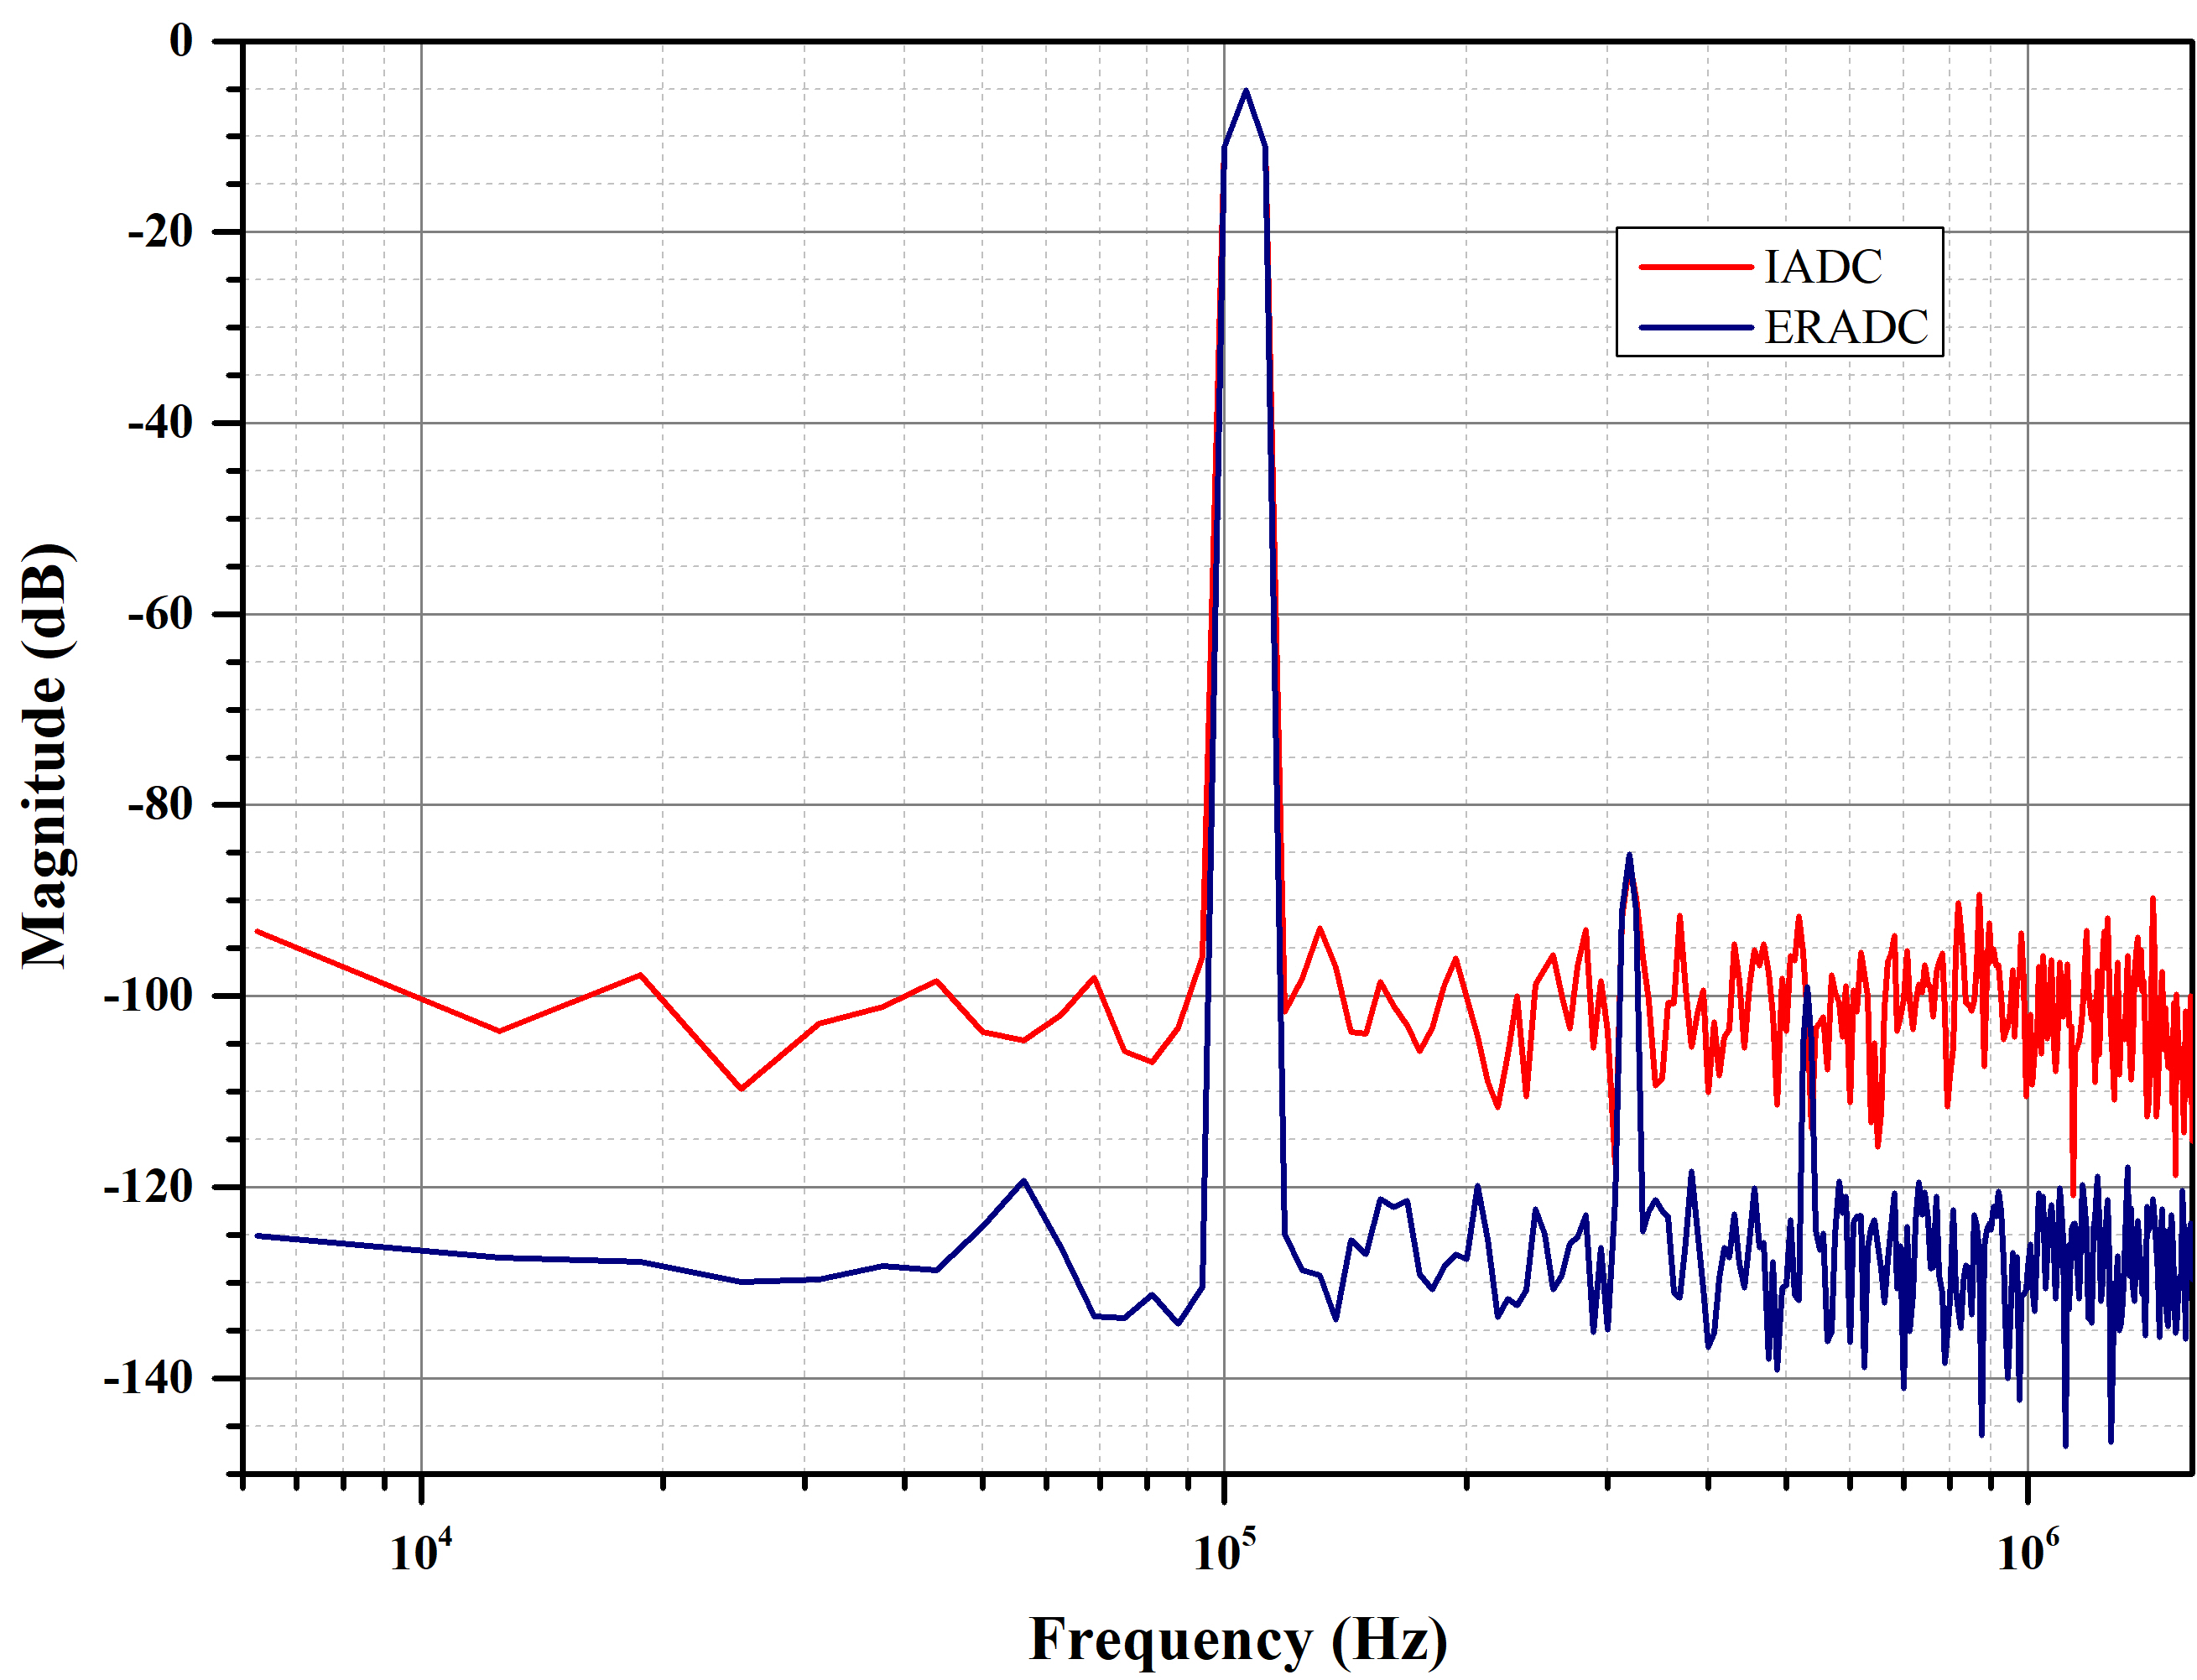
\includegraphics[width=0.8\columnwidth]{Chap06/Figures/PSD_ISDM_av.jpg}
    \caption{Post-Layout simulation Power Spectral Density of the Incremental SDM}
    \label{fig:psd_iadc_sav}
\end{figure}
%
The results of the extracted simulations are depicted in Fig.~\ref{fig:psd_iadc_sav}. With coarse quantization, the SNDR that can be achieved remains equal as that in the ideal simulation or that in the simulation with blocks at transistor level i.e. around 60~dB. However, the SNDR in case of complete architecture of ERADC deteriorates w.r.t. ideal case, to 73~dB, still maintaining the noise floor at -125~dB, in presence of harmonics.
%
\begin{figure}[h!]
    \centering
    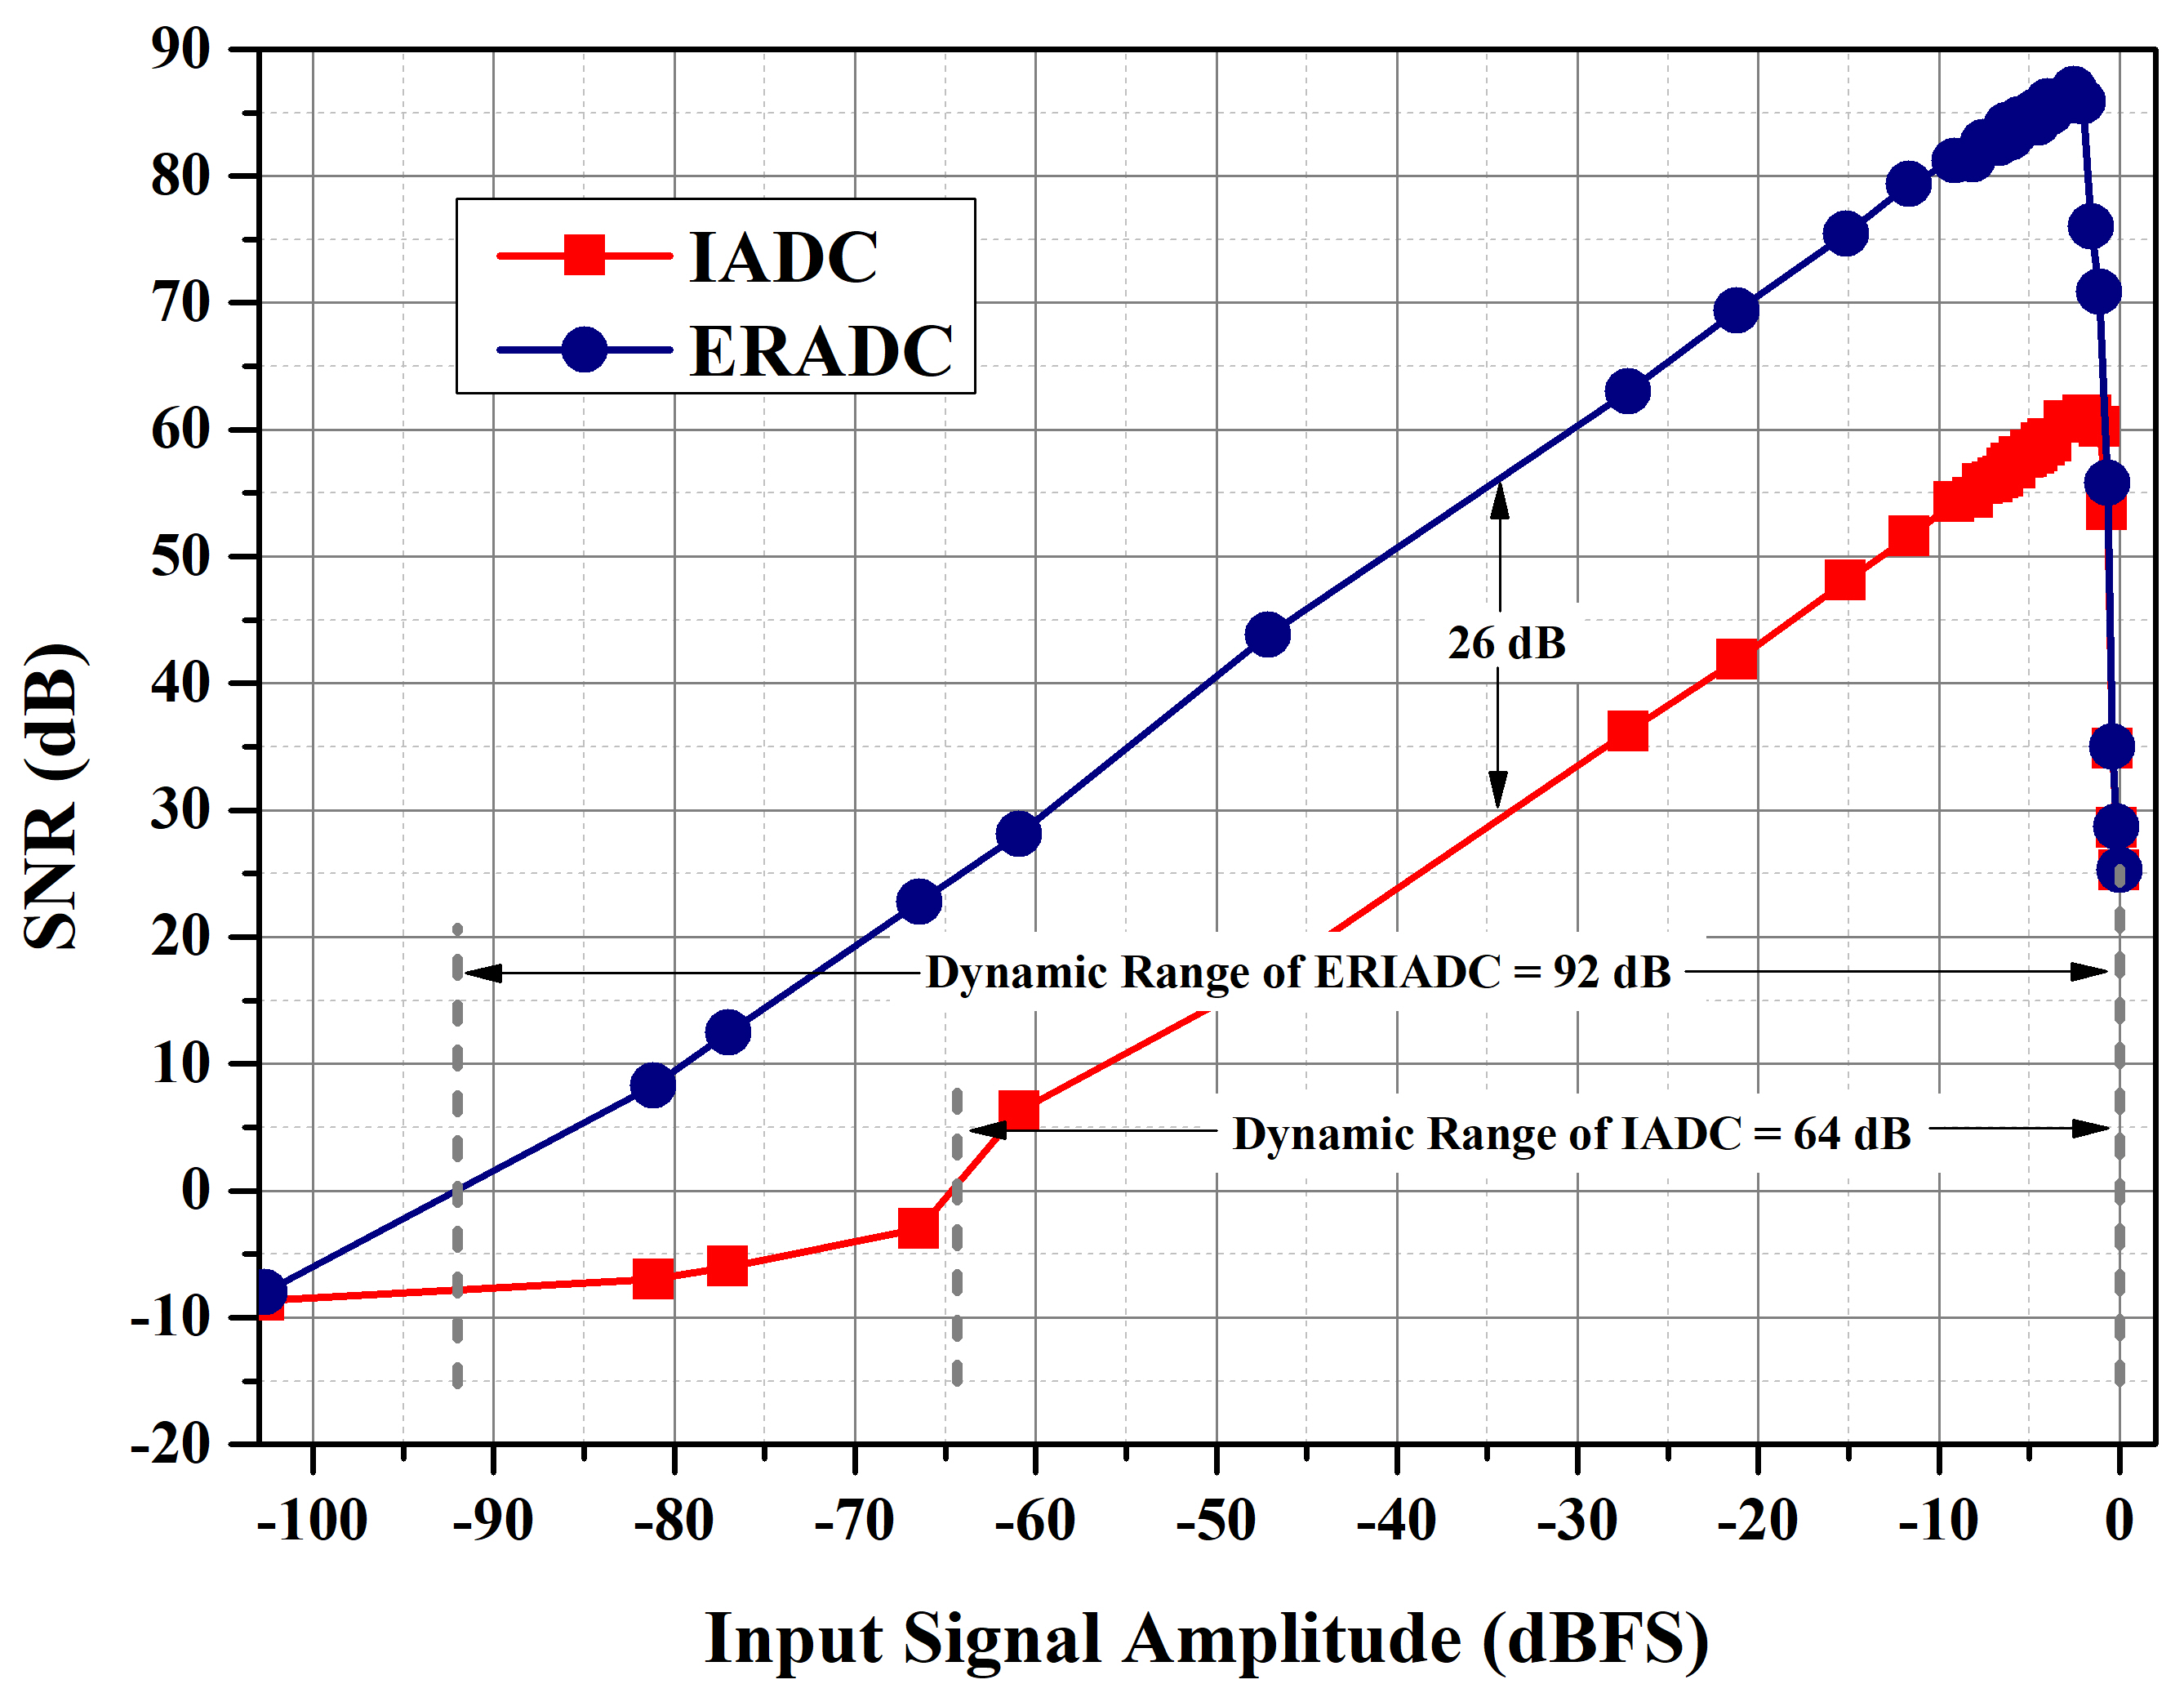
\includegraphics[width=0.8\columnwidth]{Chap06/Figures/PSD_ERADC.jpg}
    \caption{Signal-to-Noise Ratio Vs input signal amplitude of ERADC with all the blocks at transistor level design}
    \label{fig:snr_vs_input_sch}
\end{figure}
%

\section{Measurements Results}
The Incremental {\textSigma}{\textDelta} ADC has been fabricated and it's performance has also been measured. This version of the architecture is configured in two modes, Incremental mode (I-mode) and Sigma-Delta mode (SD-mode). When I-mode is active, the structure generates the RESET signal every 19 clock cycles and resets all the memory elements while in case of SD-mode, it does not generates the RESET signal thus structure runs freely maintaining the quantization noise memory. This selection of the configuration of either of the modes is done through the JTAG programming bit. 
%
\begin{figure}[h!]
    \centering
    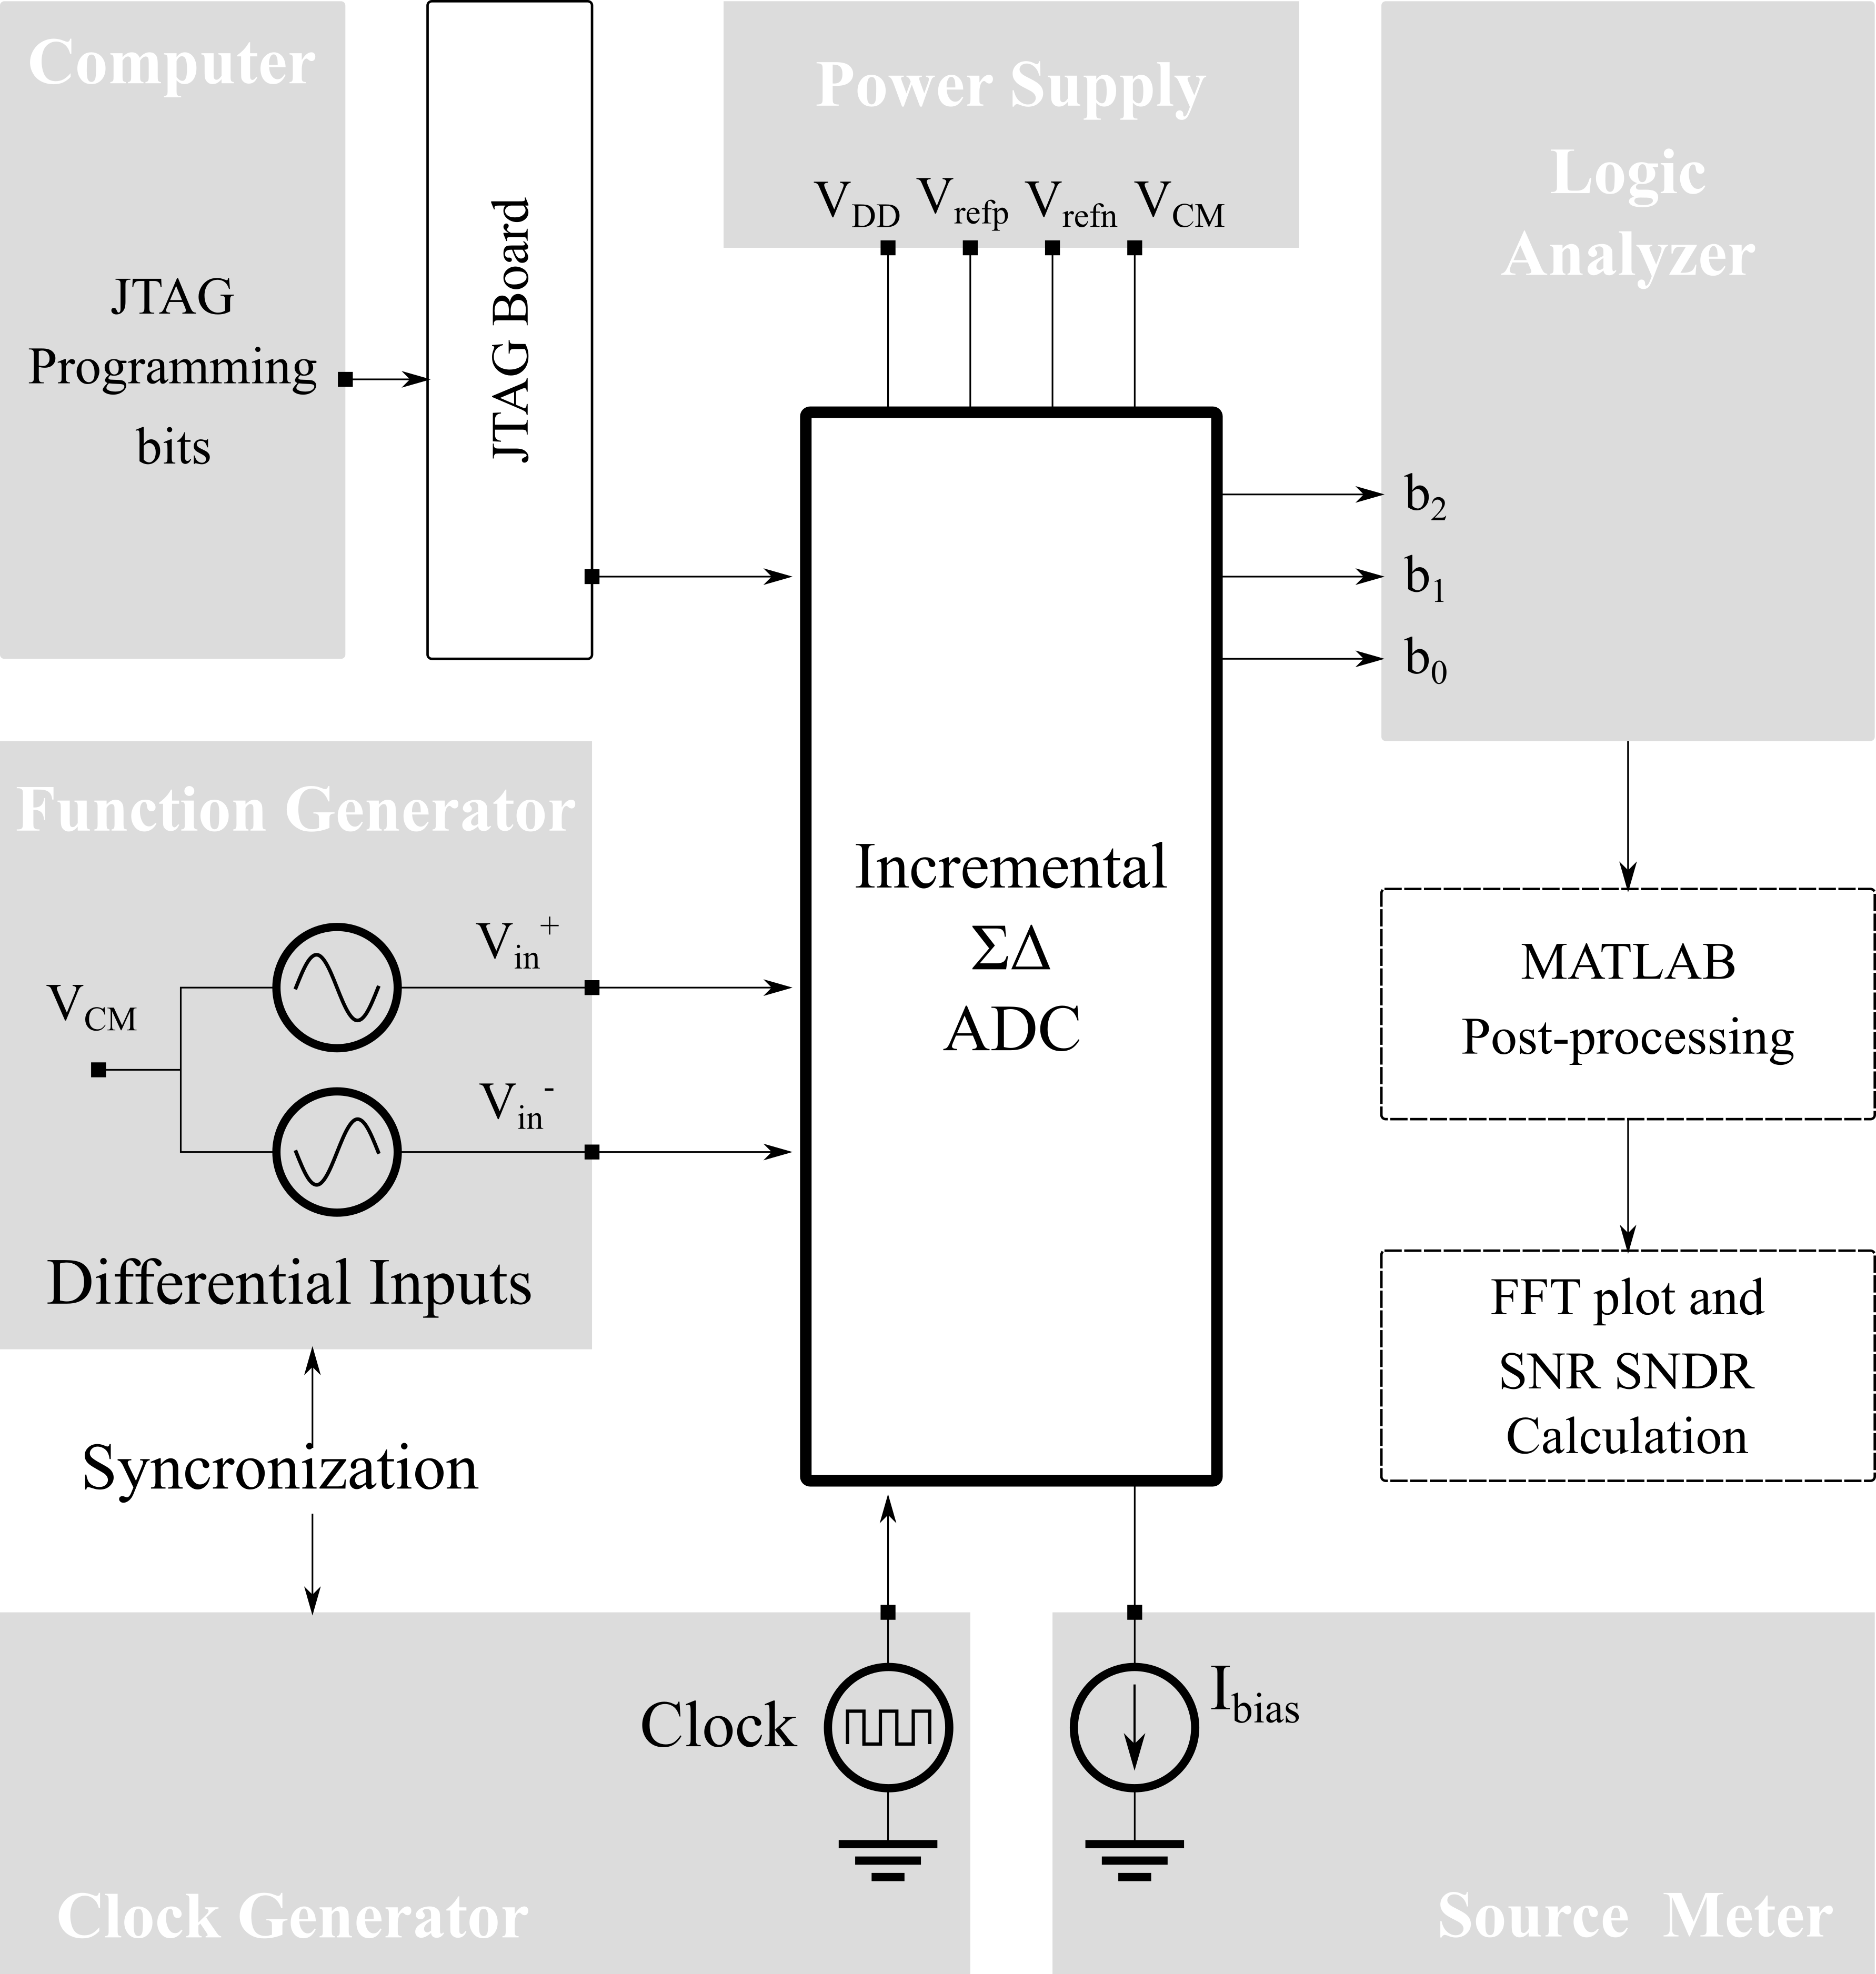
\includegraphics[width=0.85\columnwidth]{Chap06/Figures/sdm_measurement_setup.png}
    \caption{Measurement Set-up for the characterization of the Incremental (\textSigma \textDelta) ADC}
    \label{fig:meas_setup_iadc}
\end{figure}
%

The measurement set-up was done as shown in Fig.~\ref{fig:meas_setup_iadc}. For the input sinusoid, a function generator was used generating differential inputs, for square wave clock, a clock generator, a bias current drawn from the source-meter and for the DC voltages such as common-mode voltage, reference voltages, supply voltages and ground, the power supplies were used. The programming bit such as SD/I mode-selection, Power-down mode and programming bit of bias currents for op-amps and comparators in the quantizer, a JTAG programming was used. Then, once the conversion is done, the digital bit were acquired by interfacing Logic analyzer and the text file was created. Further post-processing was done in the MATLAB by importing the generated text file with output bit where the SNR, SNDR, dynamic range (DR) were calculated and FFT graphs were plotted to see the PSD of the digitized signal.

\subsection{Sigma-Delta Mode:}
%
\begin{figure}[h!]
    \centering
    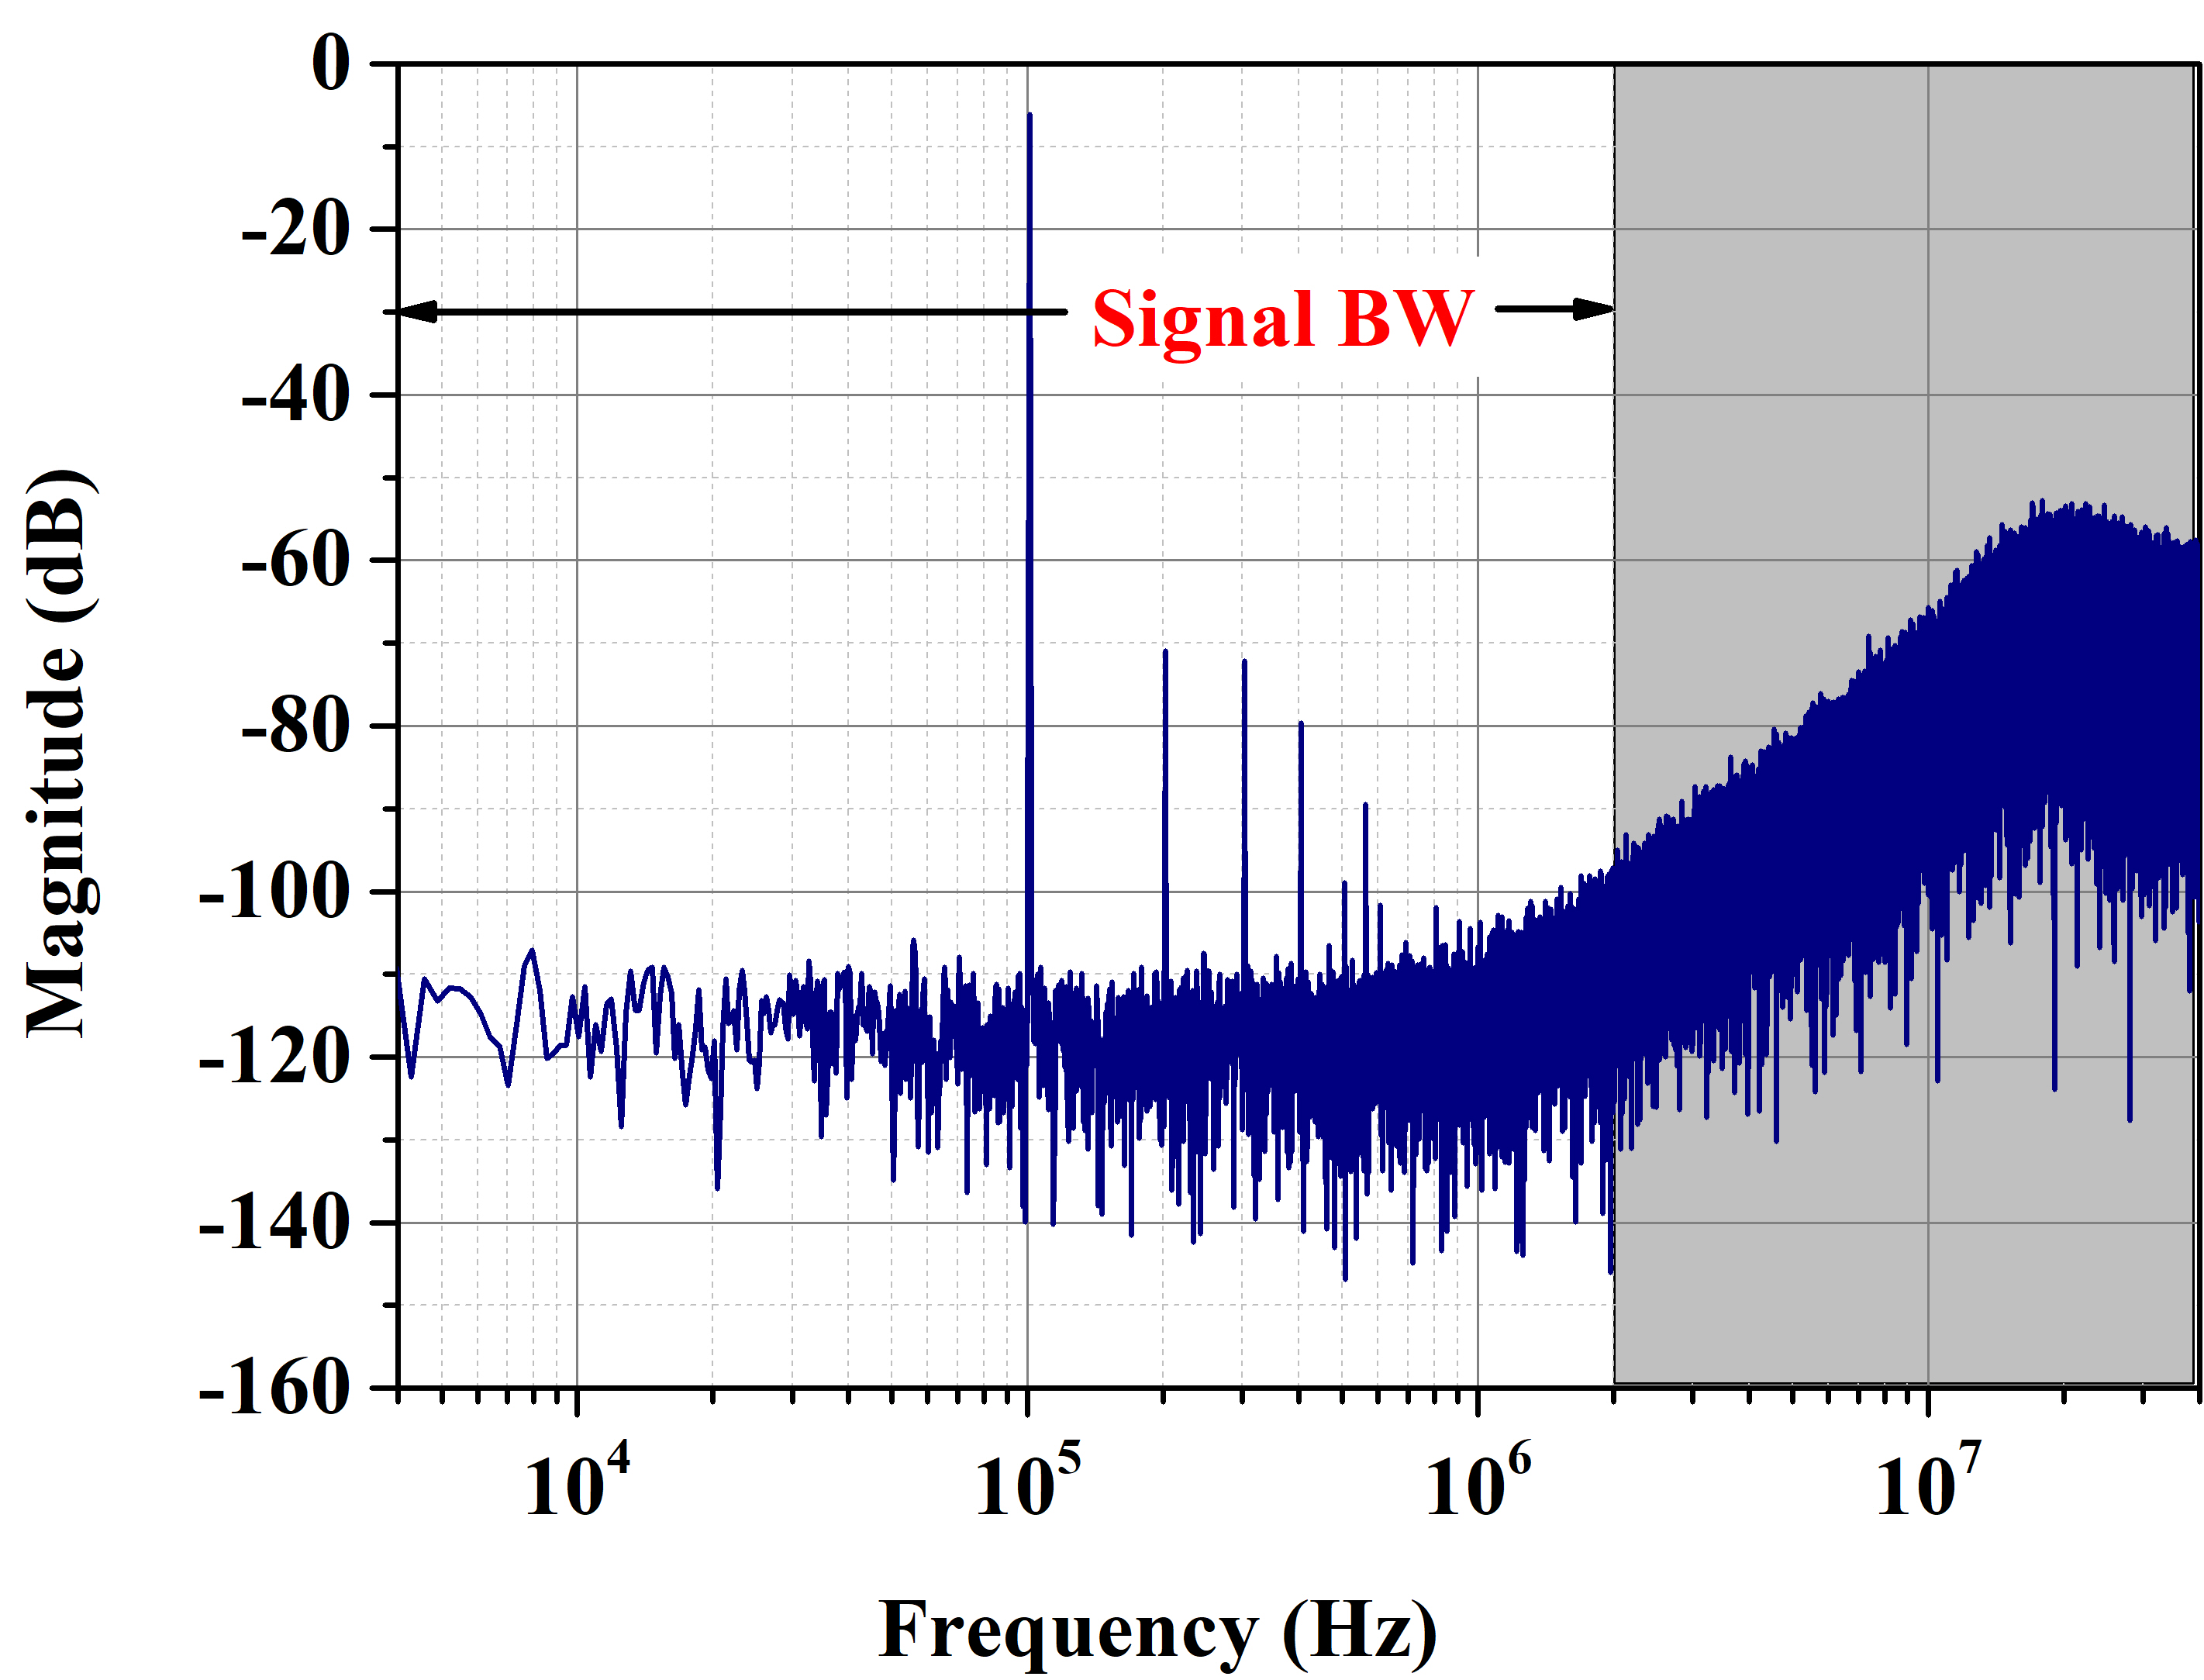
\includegraphics[width=0.8\columnwidth]{Chap06/Figures/PSD_SDM_meas.jpg}
    \caption{PSD of the Sigma-Delta (\textSigma \textDelta) ADC}
    \label{fig:sdm_psd}
\end{figure}
%

Fig. \ref{fig:sdm_psd}, \ref{fig:sdm_psd} and \ref{fig:sdm_snr_vs_osr} shows the measurements results of the architecture when configured in the sigma-delta mode. Fig. \ref{fig:sdm_psd} is the output spectrum of the signal when the input signal is applied at a frequency of 100~kHz with an amplitude of around -6~dB with respect to the full-scale and the clock frequency is 80~MHz. For the measurement of the parameters like SNR, SNDR and DR, the signal bandwidth taken into account was 2~MHz. In the output spectrum, along with input tone, few harmonics are also present and the justification for the even harmonic lies in the absence of input buffer whereas for odd harmonics, it is the mismatch in the unit elements of the feedback DAC. The \ SNDR obtained in this case is 60.7~dB, SNR of 66.4~dB while the dynamic range is 72.8~dB. 
% \begin{figure}[h]
%     \centering
%     \subfigure[]
%     {
%         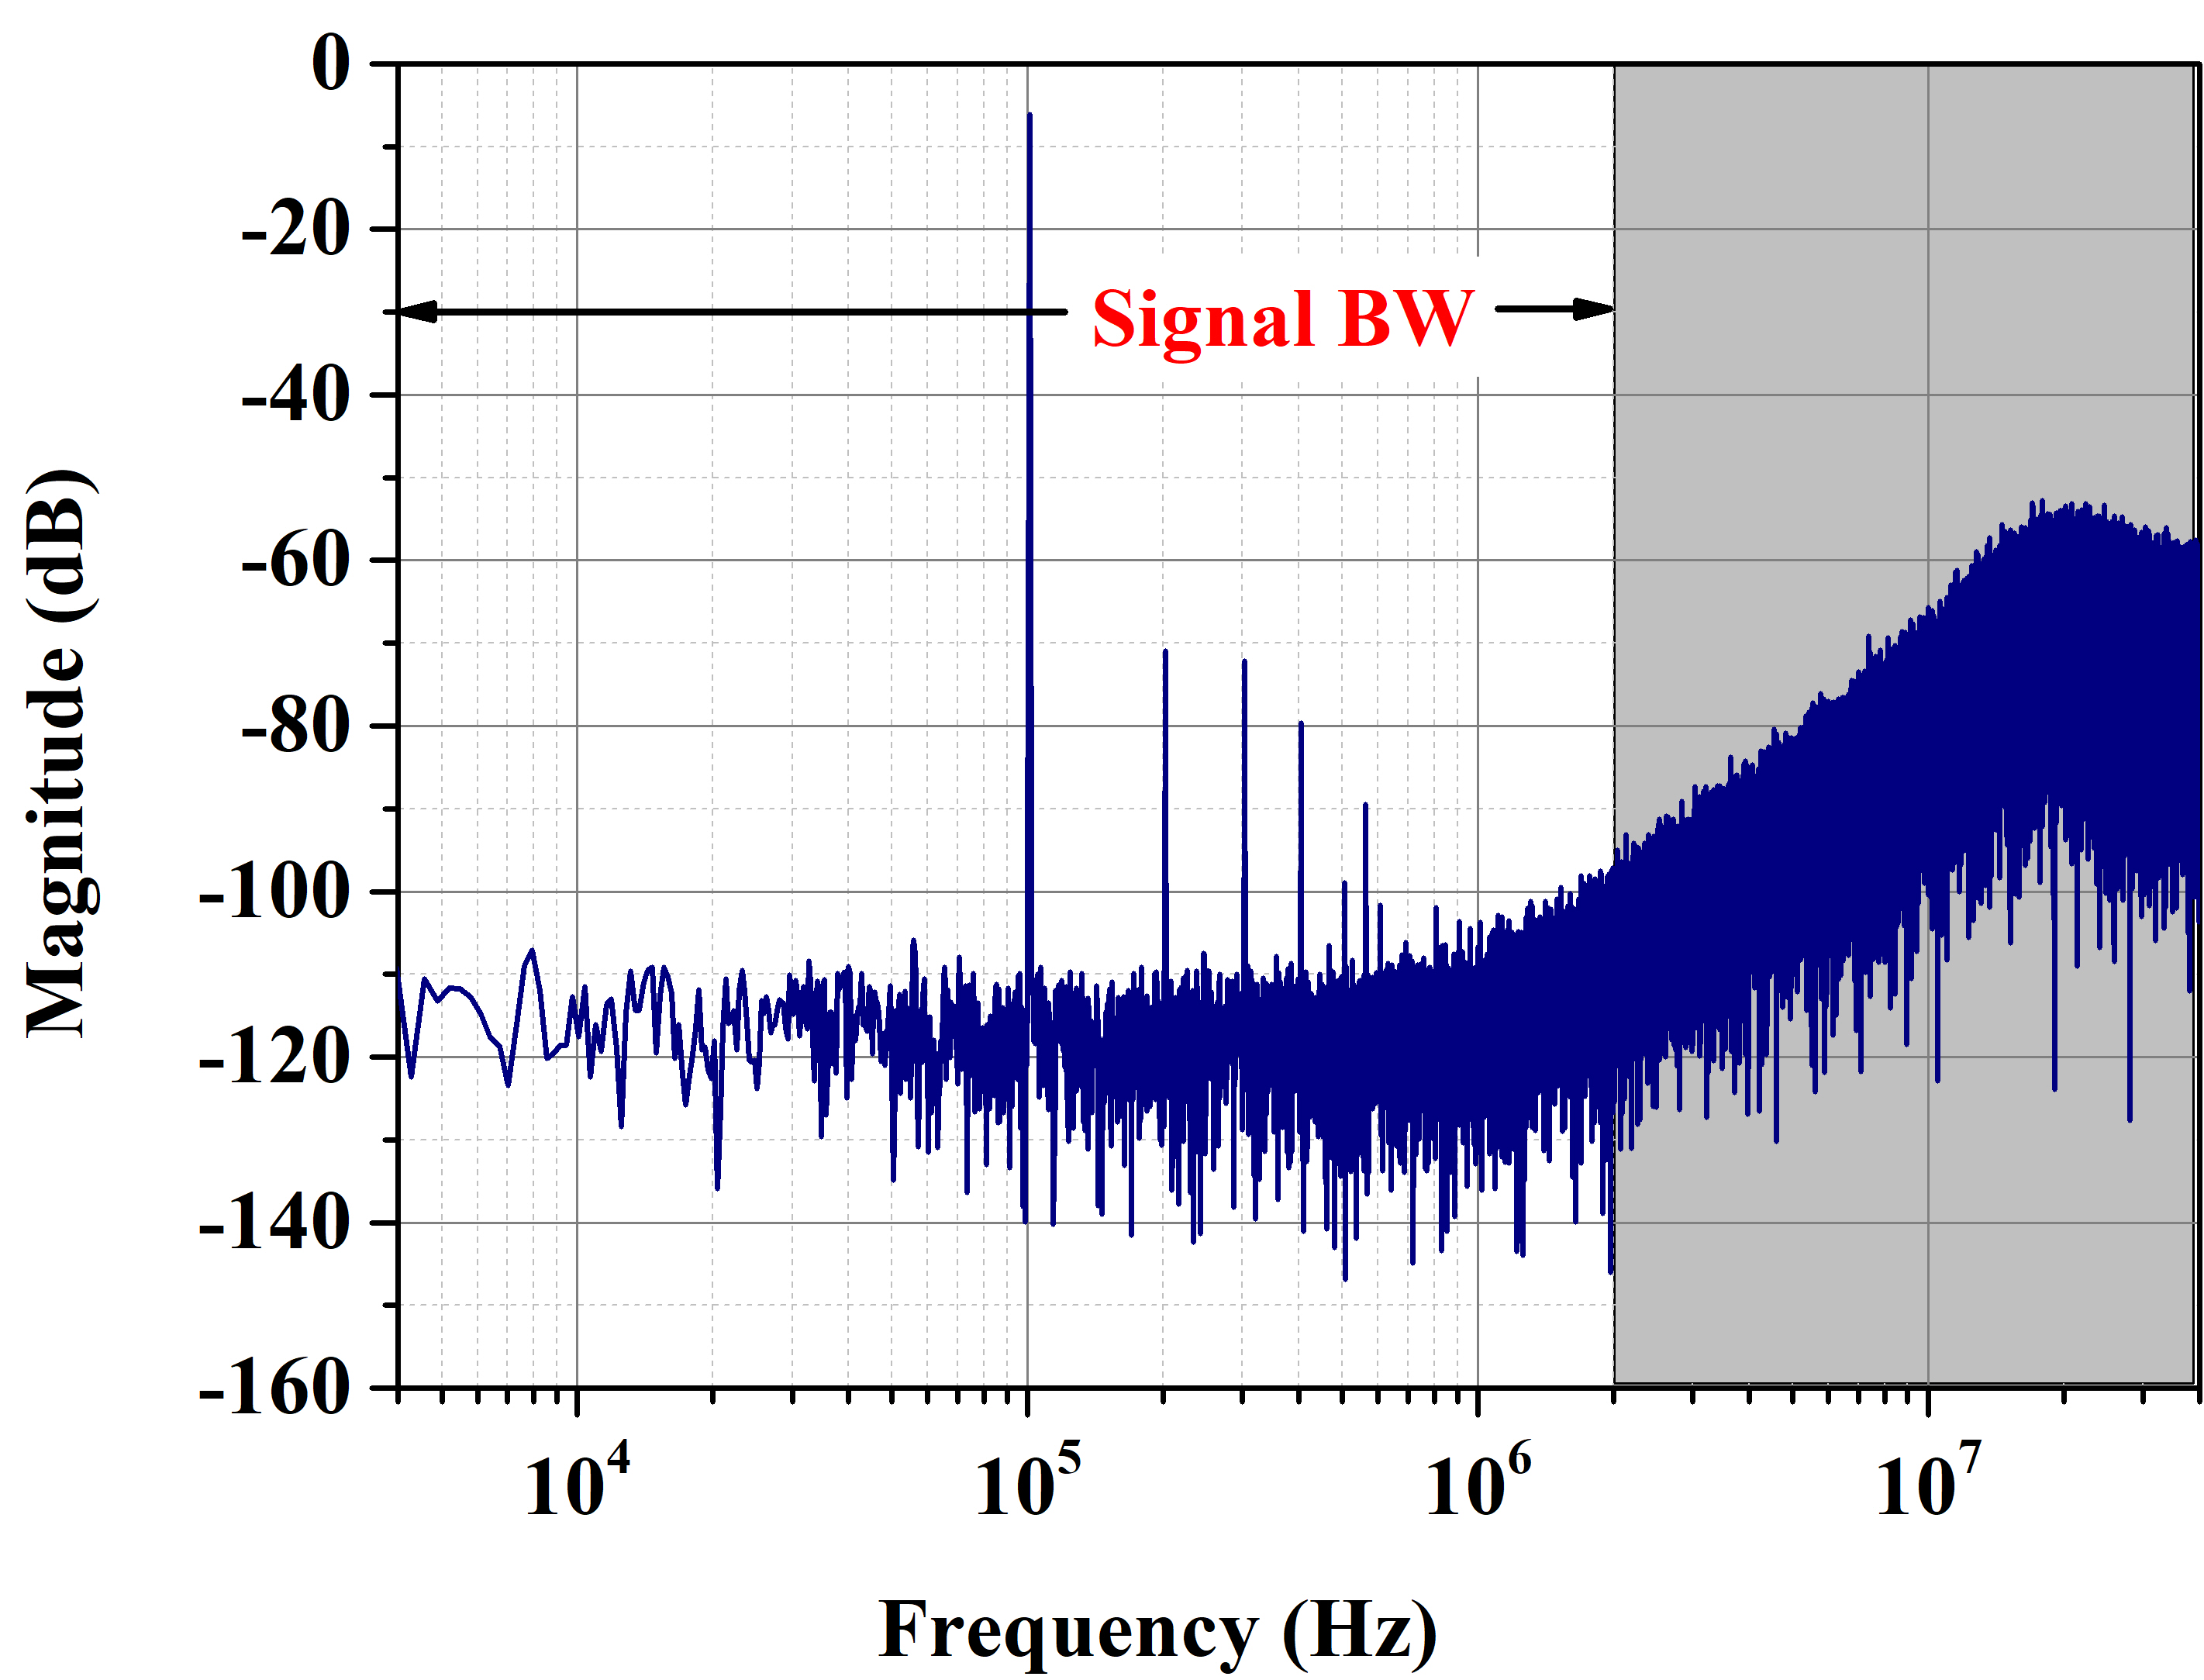
\includegraphics[scale=.27]{Chap06/Figures/PSD_SDM_meas.jpg}
%     }
%     \qquad
%     \subfigure[]
%     {
%         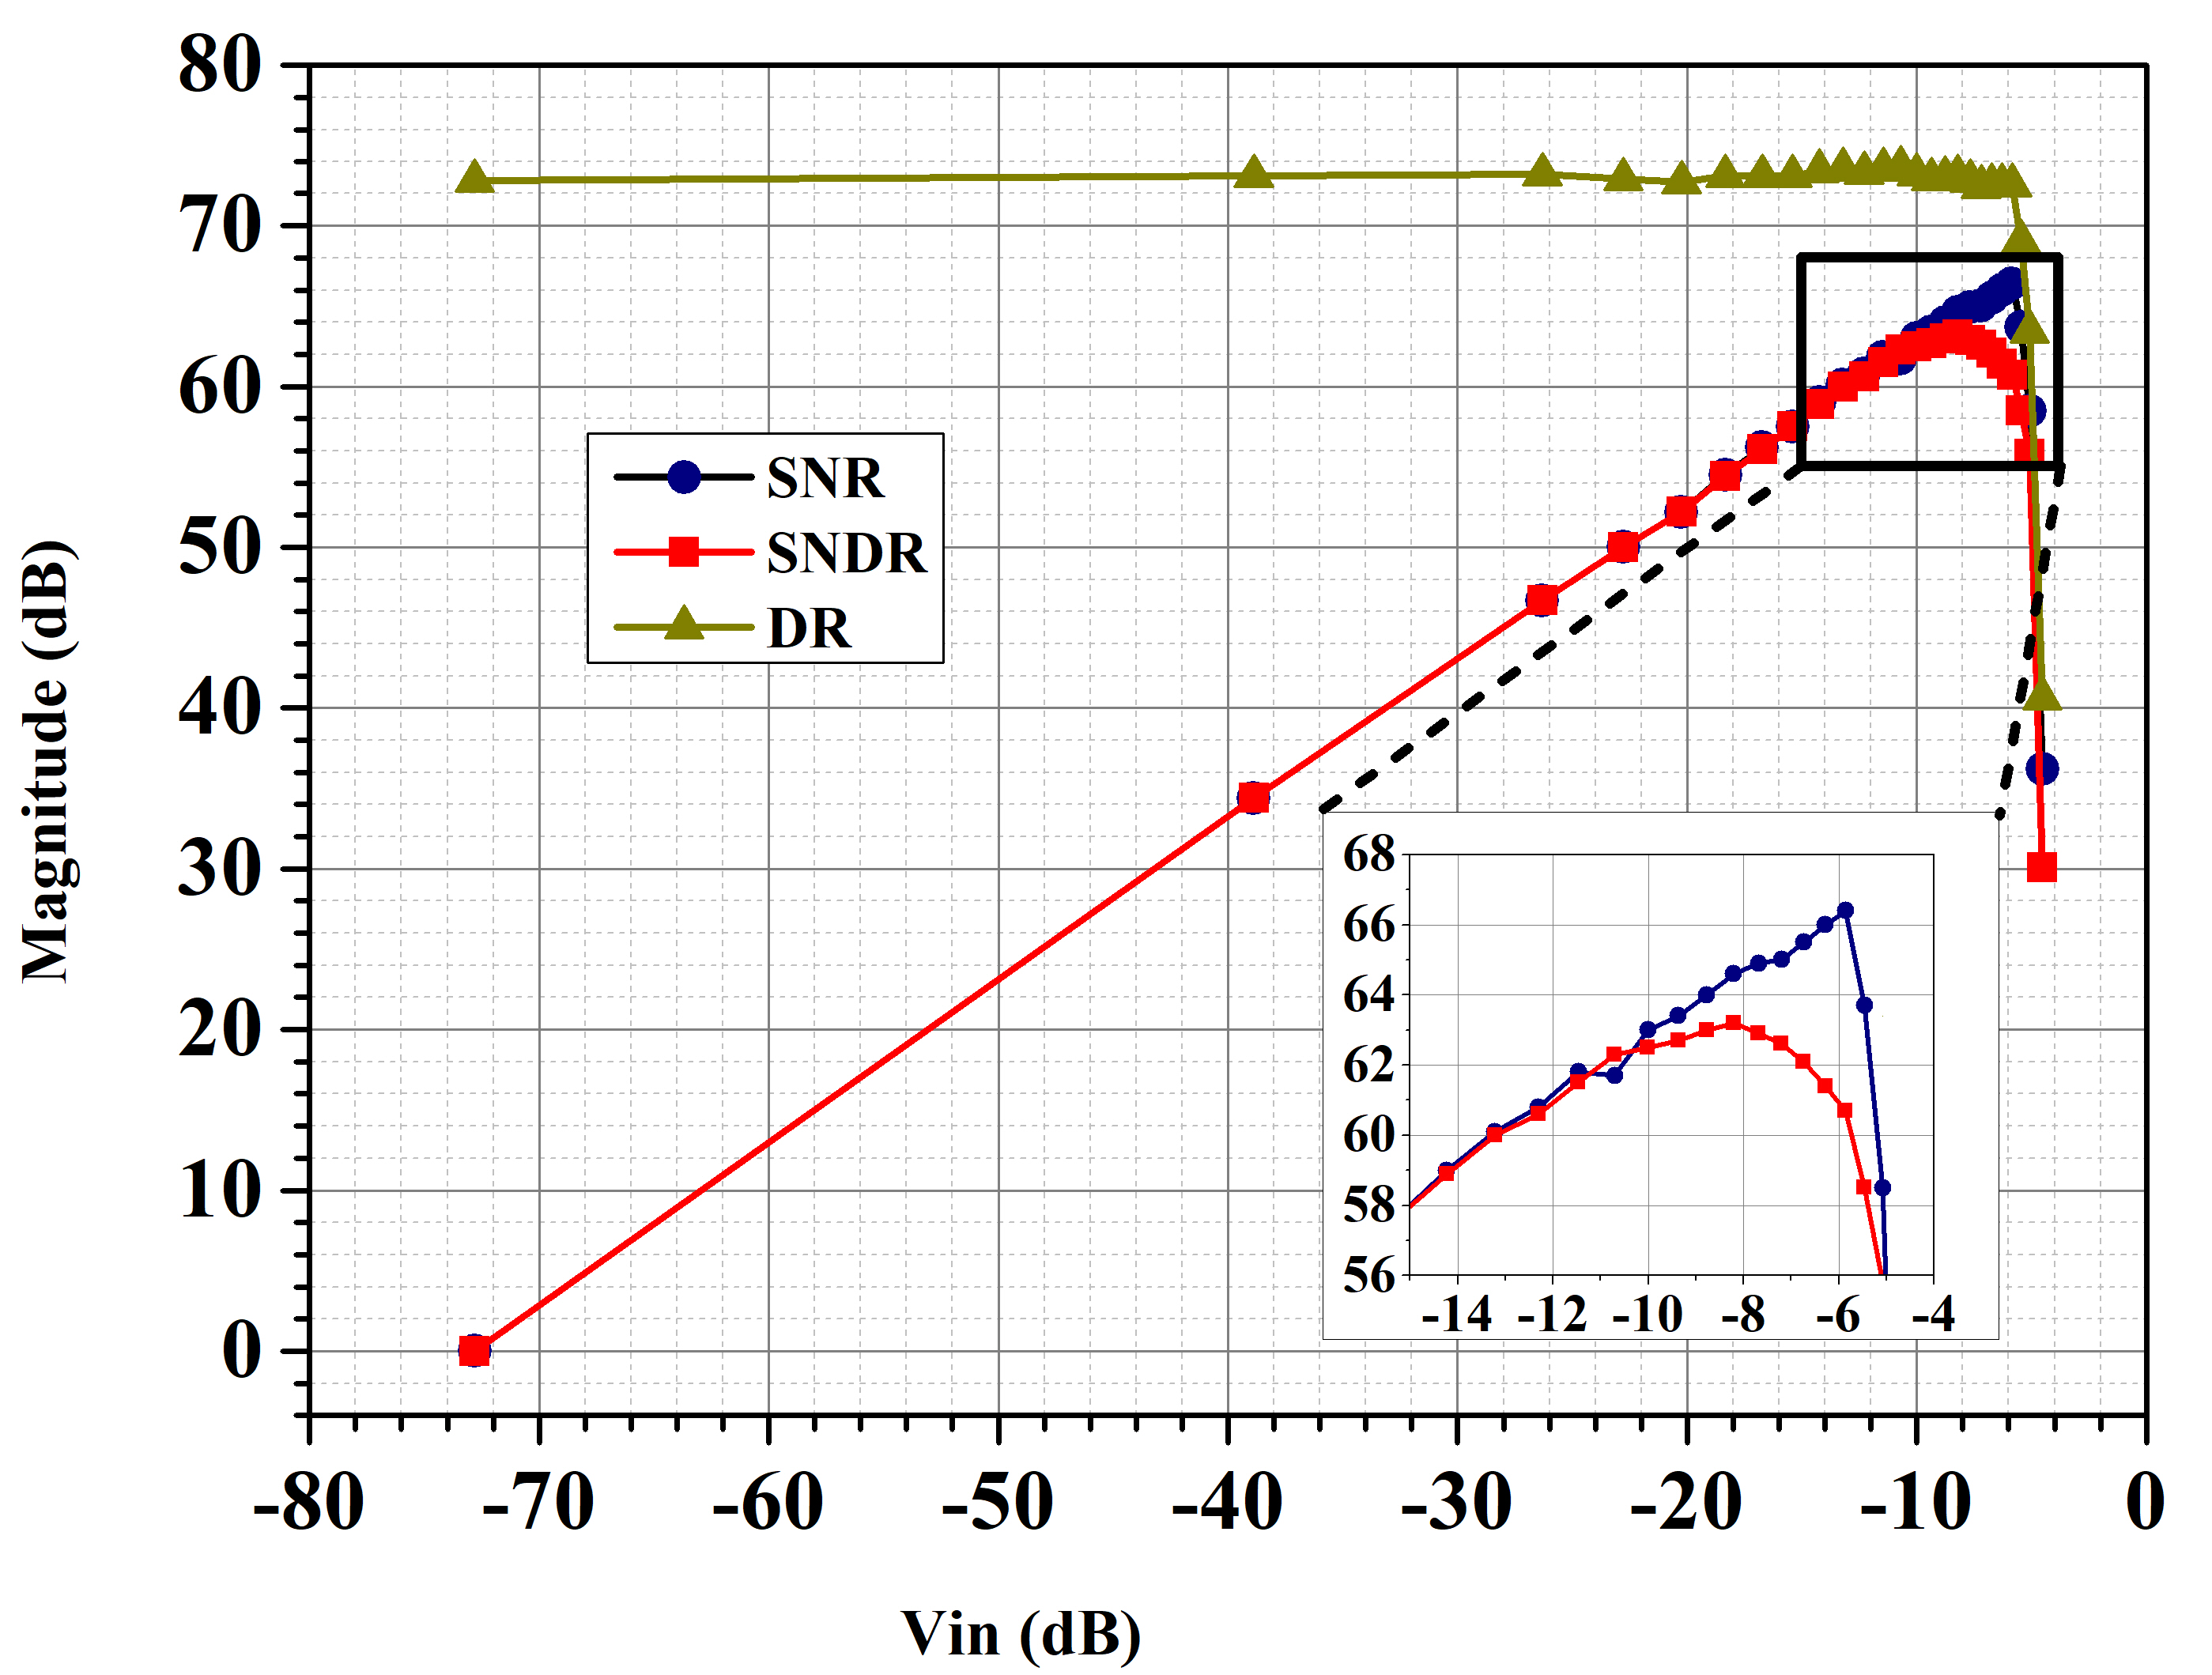
\includegraphics[scale=.27]{Chap06/Figures/snr_vs_vin_sd.jpg}
%     }
%     \caption
%     {
%         (a) PSD of the Sigma-Delta ADC
%         (b) Performance of Sigma-Delta ADC as a function of input signal amplitude
%     }
%     \label{SD_meas}
% \end{figure}
%
\begin{figure}[h!]
    \centering
    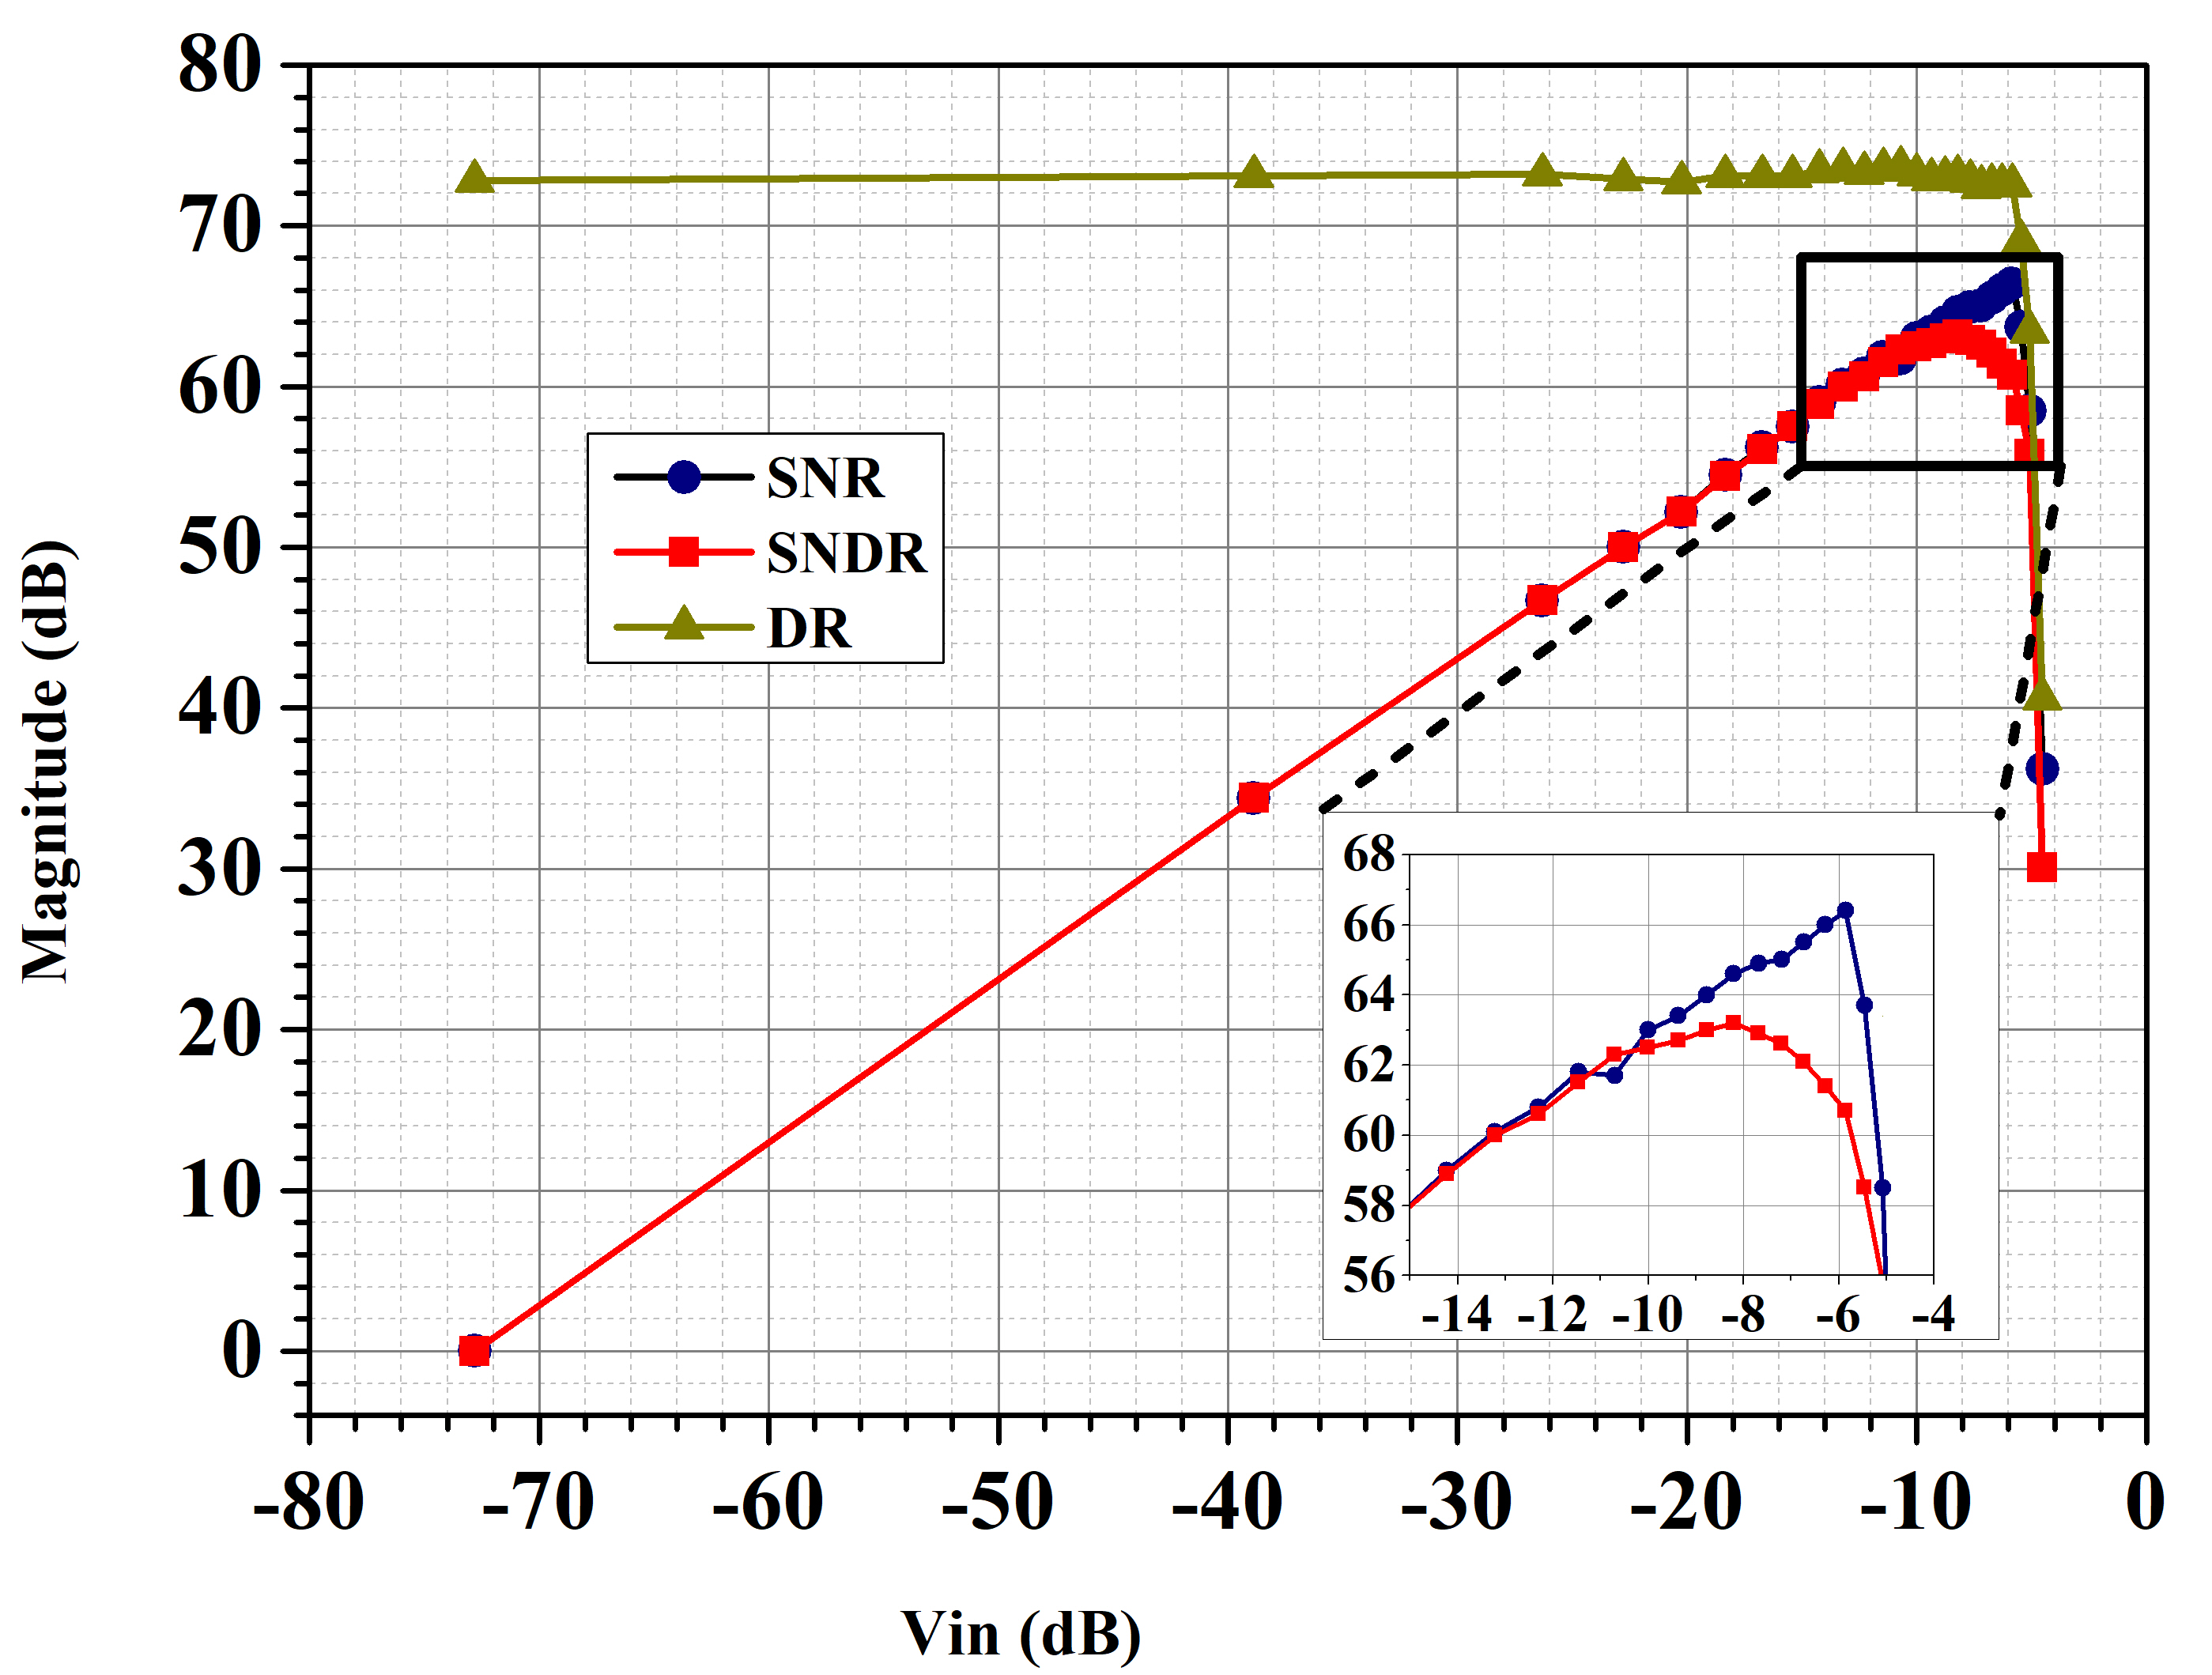
\includegraphics[width=0.8\columnwidth]{Chap06/Figures/snr_vs_vin_sd.jpg}
    \caption{Performance of \textSigma \textDelta ADC as a function of input signal amplitude }
    \label{fig:sdm_psd}
\end{figure}
%

Fig.~\ref{fig:sdm_psd} shows the SNDR, SNR and DR as a function of input signal amplitude. The maximum SNR obtained is 66.4~dB at an input amplitude of -6~dB hence an MAS (Maximum Stable Amplitude). When the amplitude of the signal is increased from -10~dB to -6~dB, the power of the harmonics goes on increasing causing a harmonic distortion. Therefore, SNDR characteristic starts deviating down from the SNR one. Further increase in the amplitude transgresses the MSA causing input dependent instability giving rise to nonlinear behaviour of the ADC, thus a significant drop in the performance as shown in the subplot of Fig.~\ref{fig:sdm_psd}.

%
\begin{figure}[h!]
    \centering
    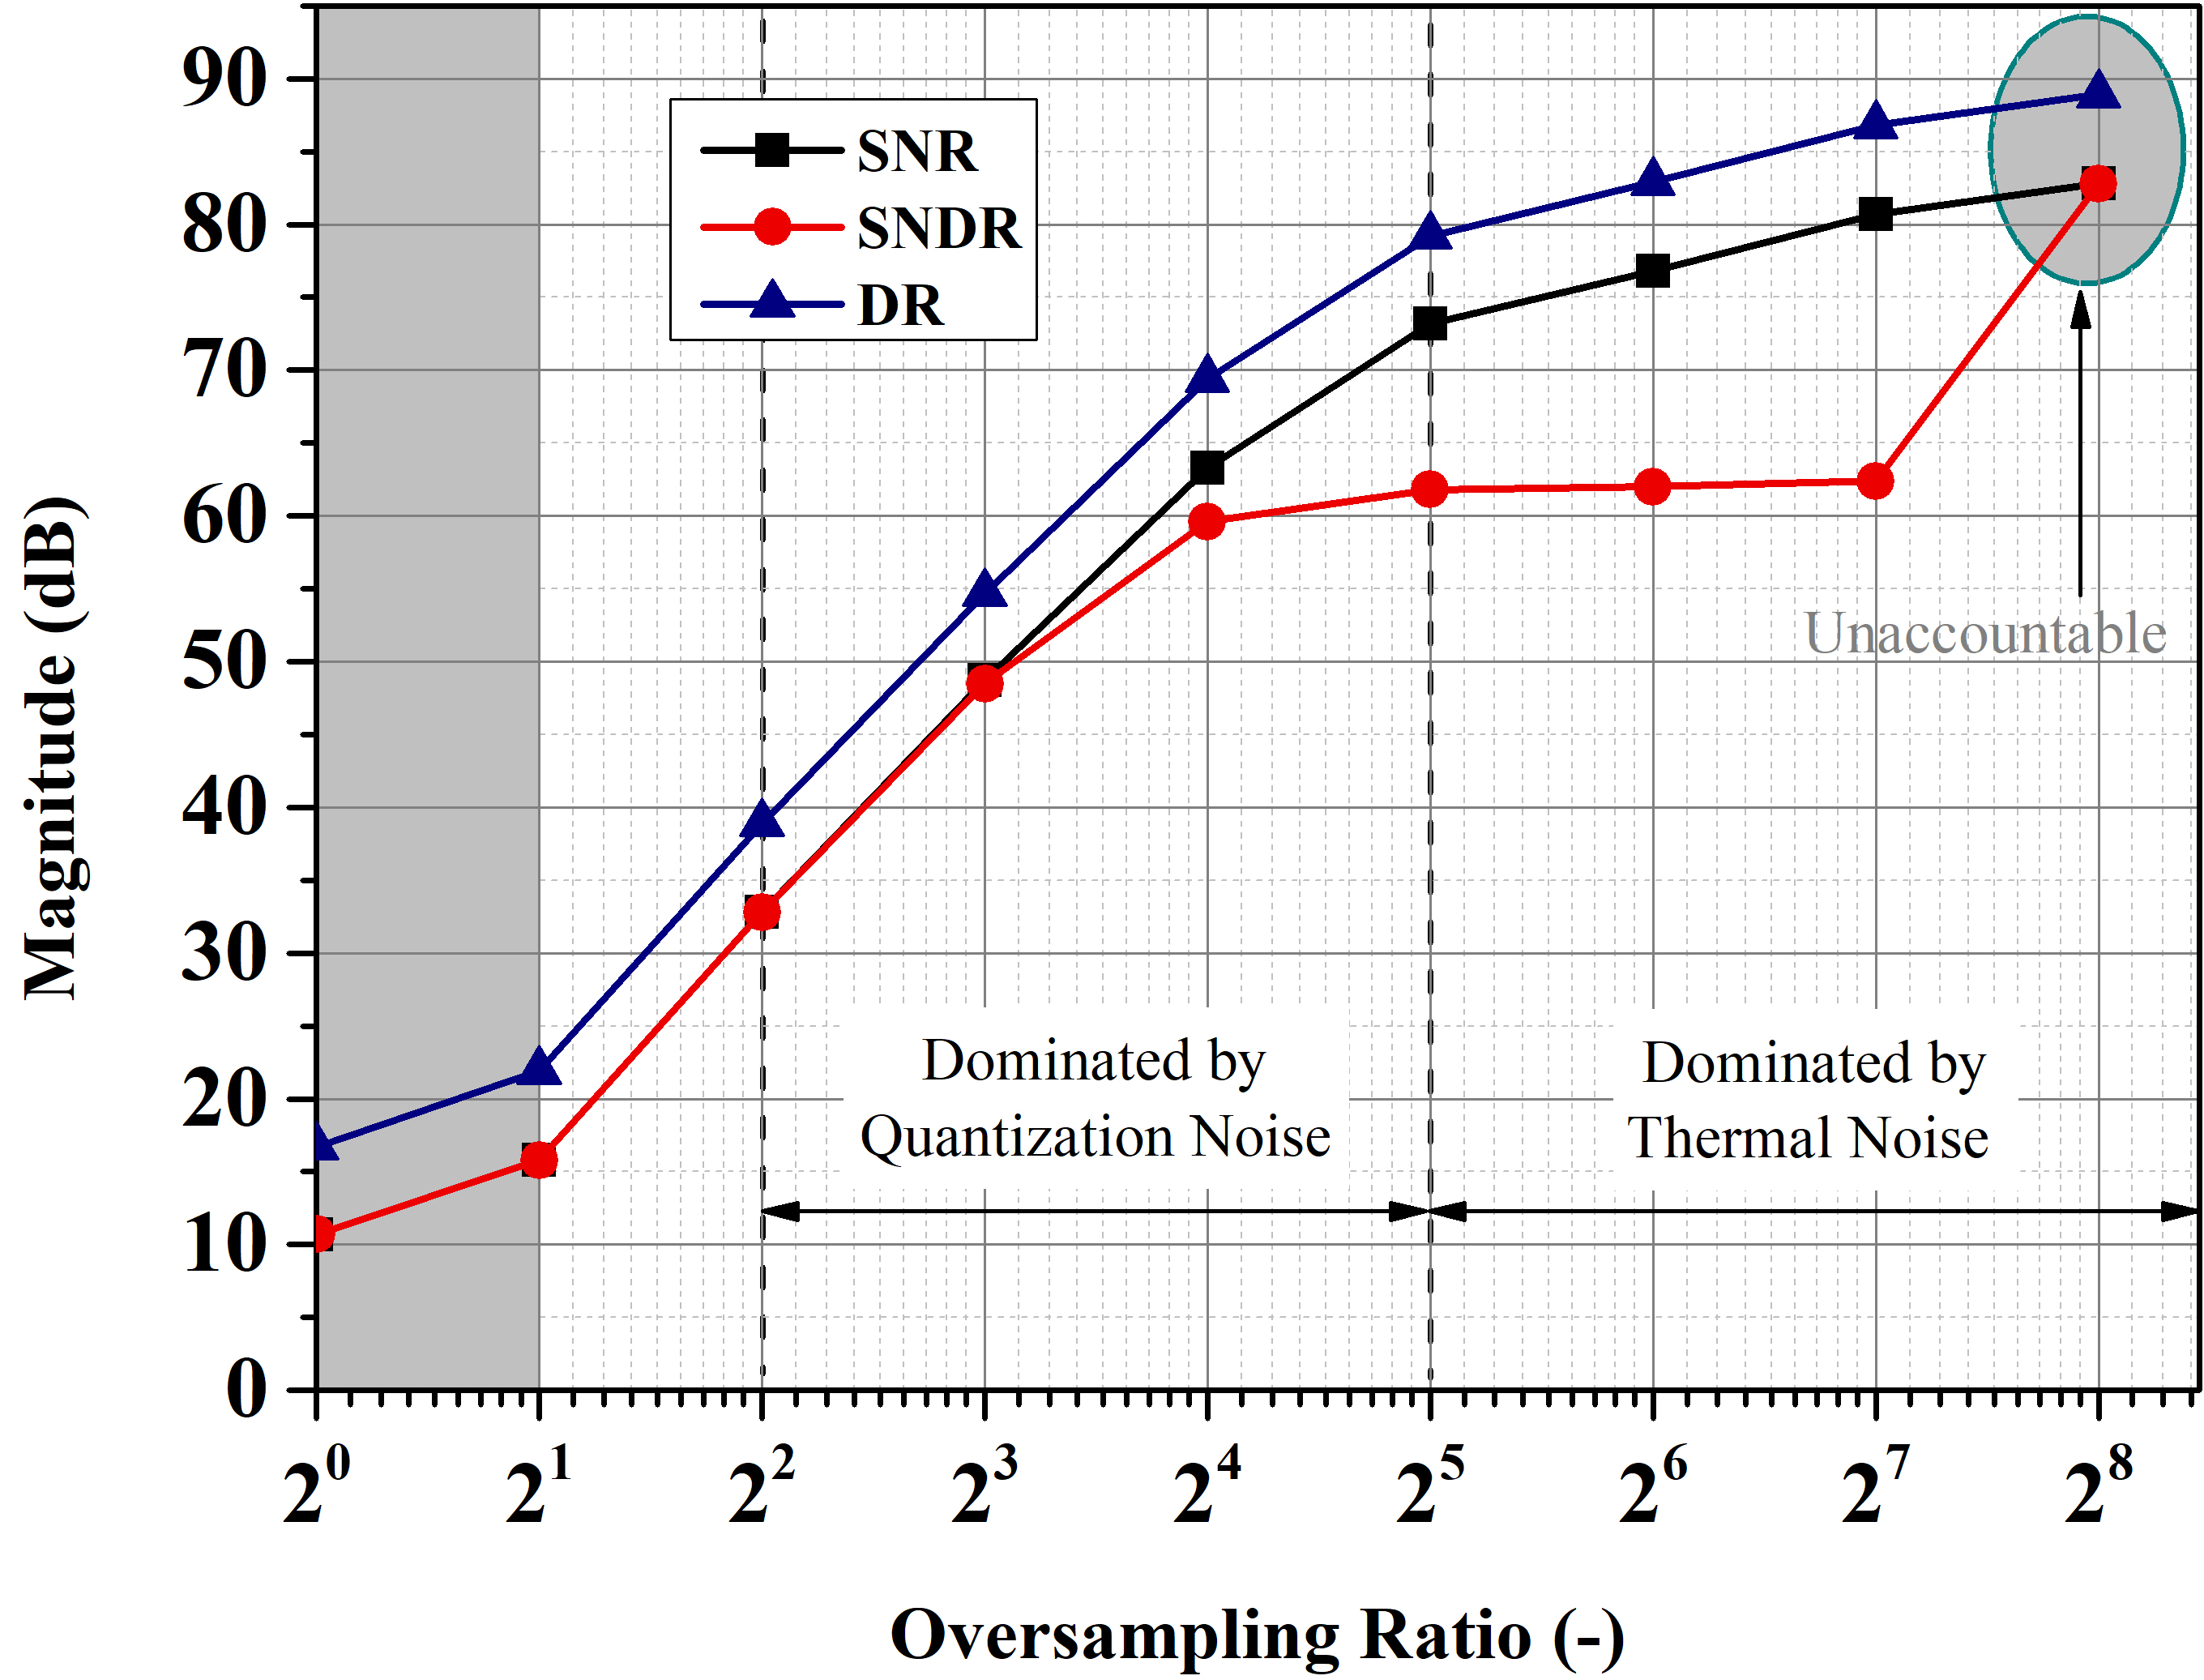
\includegraphics[width=0.8\columnwidth]{Chap06/Figures/snr_vs_osr_sd.jpg}
    \caption{Performance of \textSigma \textDelta ADC as a function of input signal amplitude }
    \label{fig:sdm_snr_vs_osr}
\end{figure}
%
The performance of the architecture in Sigma-Delta mode is also evaluated w.r.t. the oversampling ratio and can be verified by in-band noise expression of the second-order \textSigma \textDelta ADC given by Eq.~\ref{eq:in_band_noise},
%
\begin{equation}\label{eq:in_band_noise}
    In\ Band\ Noise =\frac{\Delta^2}{12\pi}\frac{1}{5}\left(\frac{\pi}{M}\right)^5
\end{equation}
%
where, \textDelta is LSB of the quantizer and $M$ is the oversampling ratio.
The above Eq.~\ref{eq:in_band_noise} indicates that for every doubling of the OSR i.e. $M$, the quantization noise goes down by a factor of 32 i.e. 15~dB. 

As depicted in Fig.~\ref{fig:sdm_snr_vs_osr}, in the range from OSR value $2^2$ to $2^5$, the SNR is dominated by the quantization noise (i.e. region with noise shaping with slope of -40~dB/decade). This can be observed in Fig.~\ref{fig:sdm_psd}, from frequency 1~MHz to 20~MHz. In this region, for every doubling of the OSR value, there is improvement in SNR by a factor of 15~dB, thus analysis result matches with the outcome from equation Eq.~\ref{eq:in_band_noise}.

Further, when there is an increase in the OSR above $2^5$, the bandwidth of noise integration gets limited to a region where the thermal noise is more dominant over SNR than the quantization noise. In Fig.~\ref{fig:sdm_psd}, it extends below frequency of 1~MHz. 

The measured SNDR at an OSR of $2^8$ is, however, not accountable. Because, in this measurement, the bandwidth taken into account for measuring noise power is less than the 200~kHz while the input signal is at 100~kHz. Therefore, this is, in fact, masking the harmonics, though they are present in the spectrum.

\subsection{Incremental Mode:}
%
\begin{figure}[h!]
    \centering
    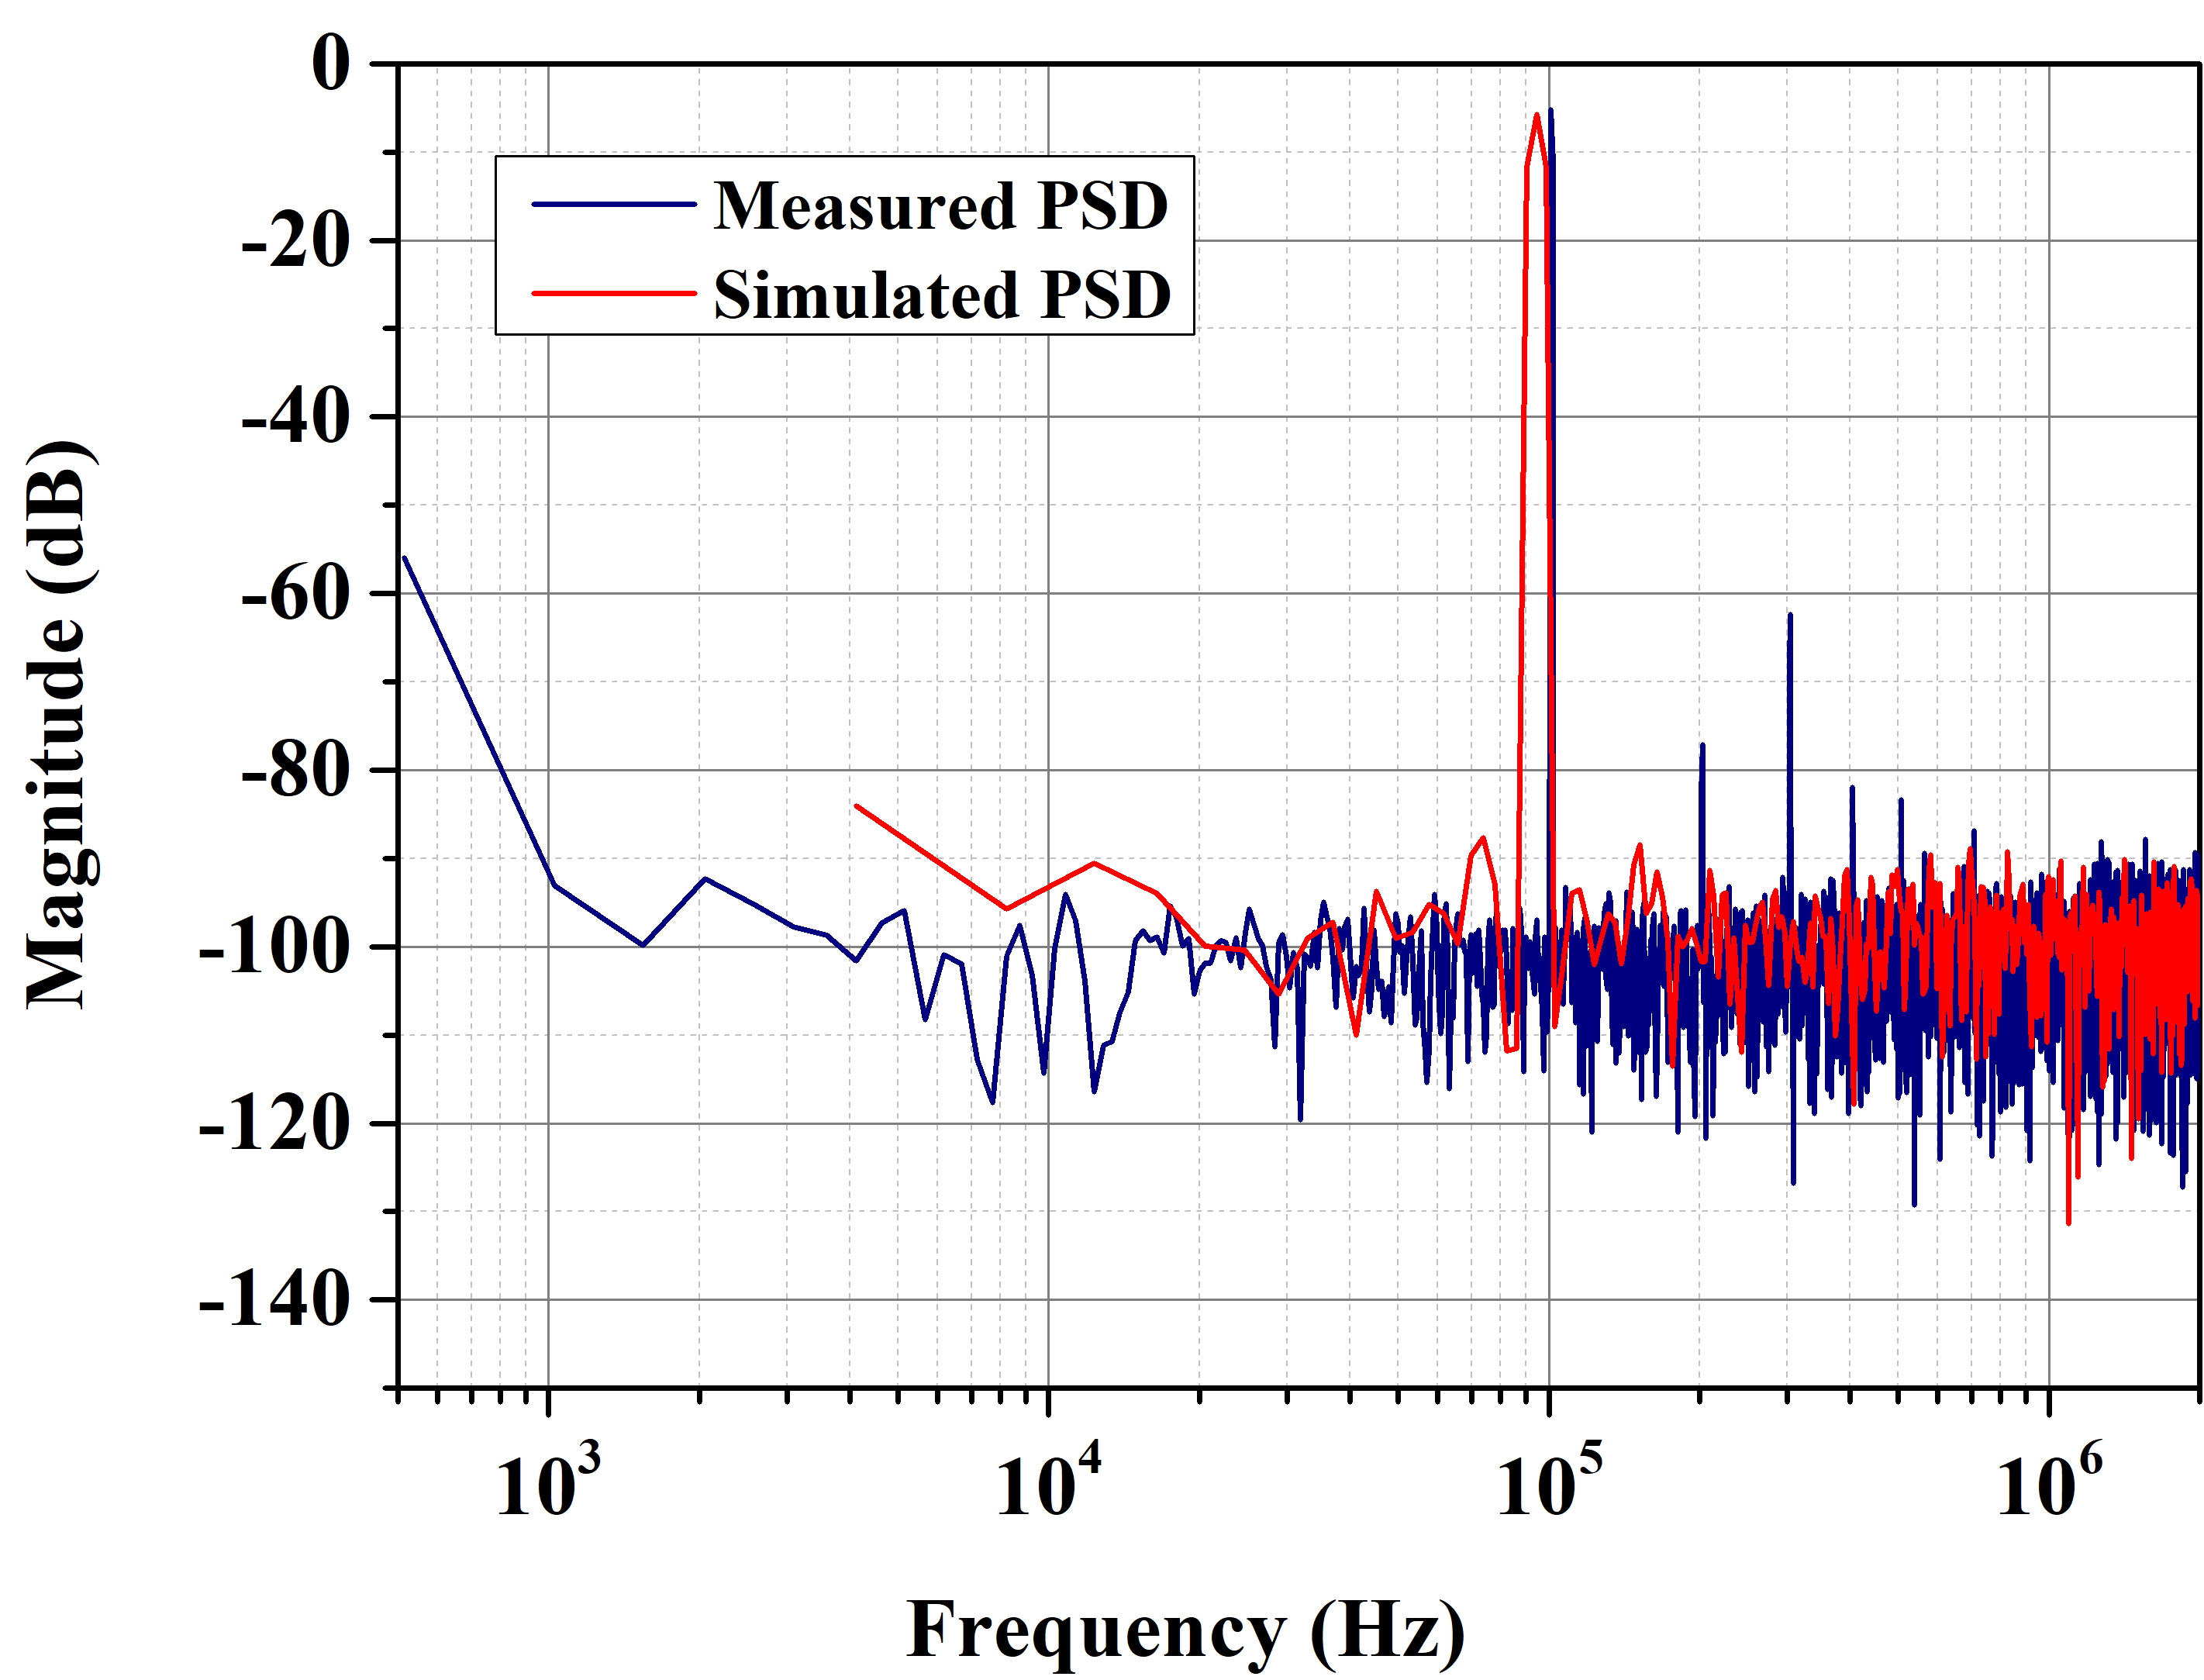
\includegraphics[width=0.8\columnwidth]{Chap06/Figures/PSD_IADC_sim_meas.jpg}
    \caption{PSD of the Incremental ADC }
    \label{fig:iadc_psd_meas}
\end{figure}
%

The output spectrum in case of Incremental mode is shown in Fig. \ref{fig:iadc_psd_meas}. The RESET feature incorporated to make the ADC accessible for multiple input sources in incremental mode erases the quantization noise memory from the integrators. The reason behind the fact that IADC PSD does not exhibit the noise shaping is the reset (loss of noise memory) along with decimation filtering (Fig. \ref{fig:iadc_psd_meas}).

%
\begin{figure}[h!]
    \centering
    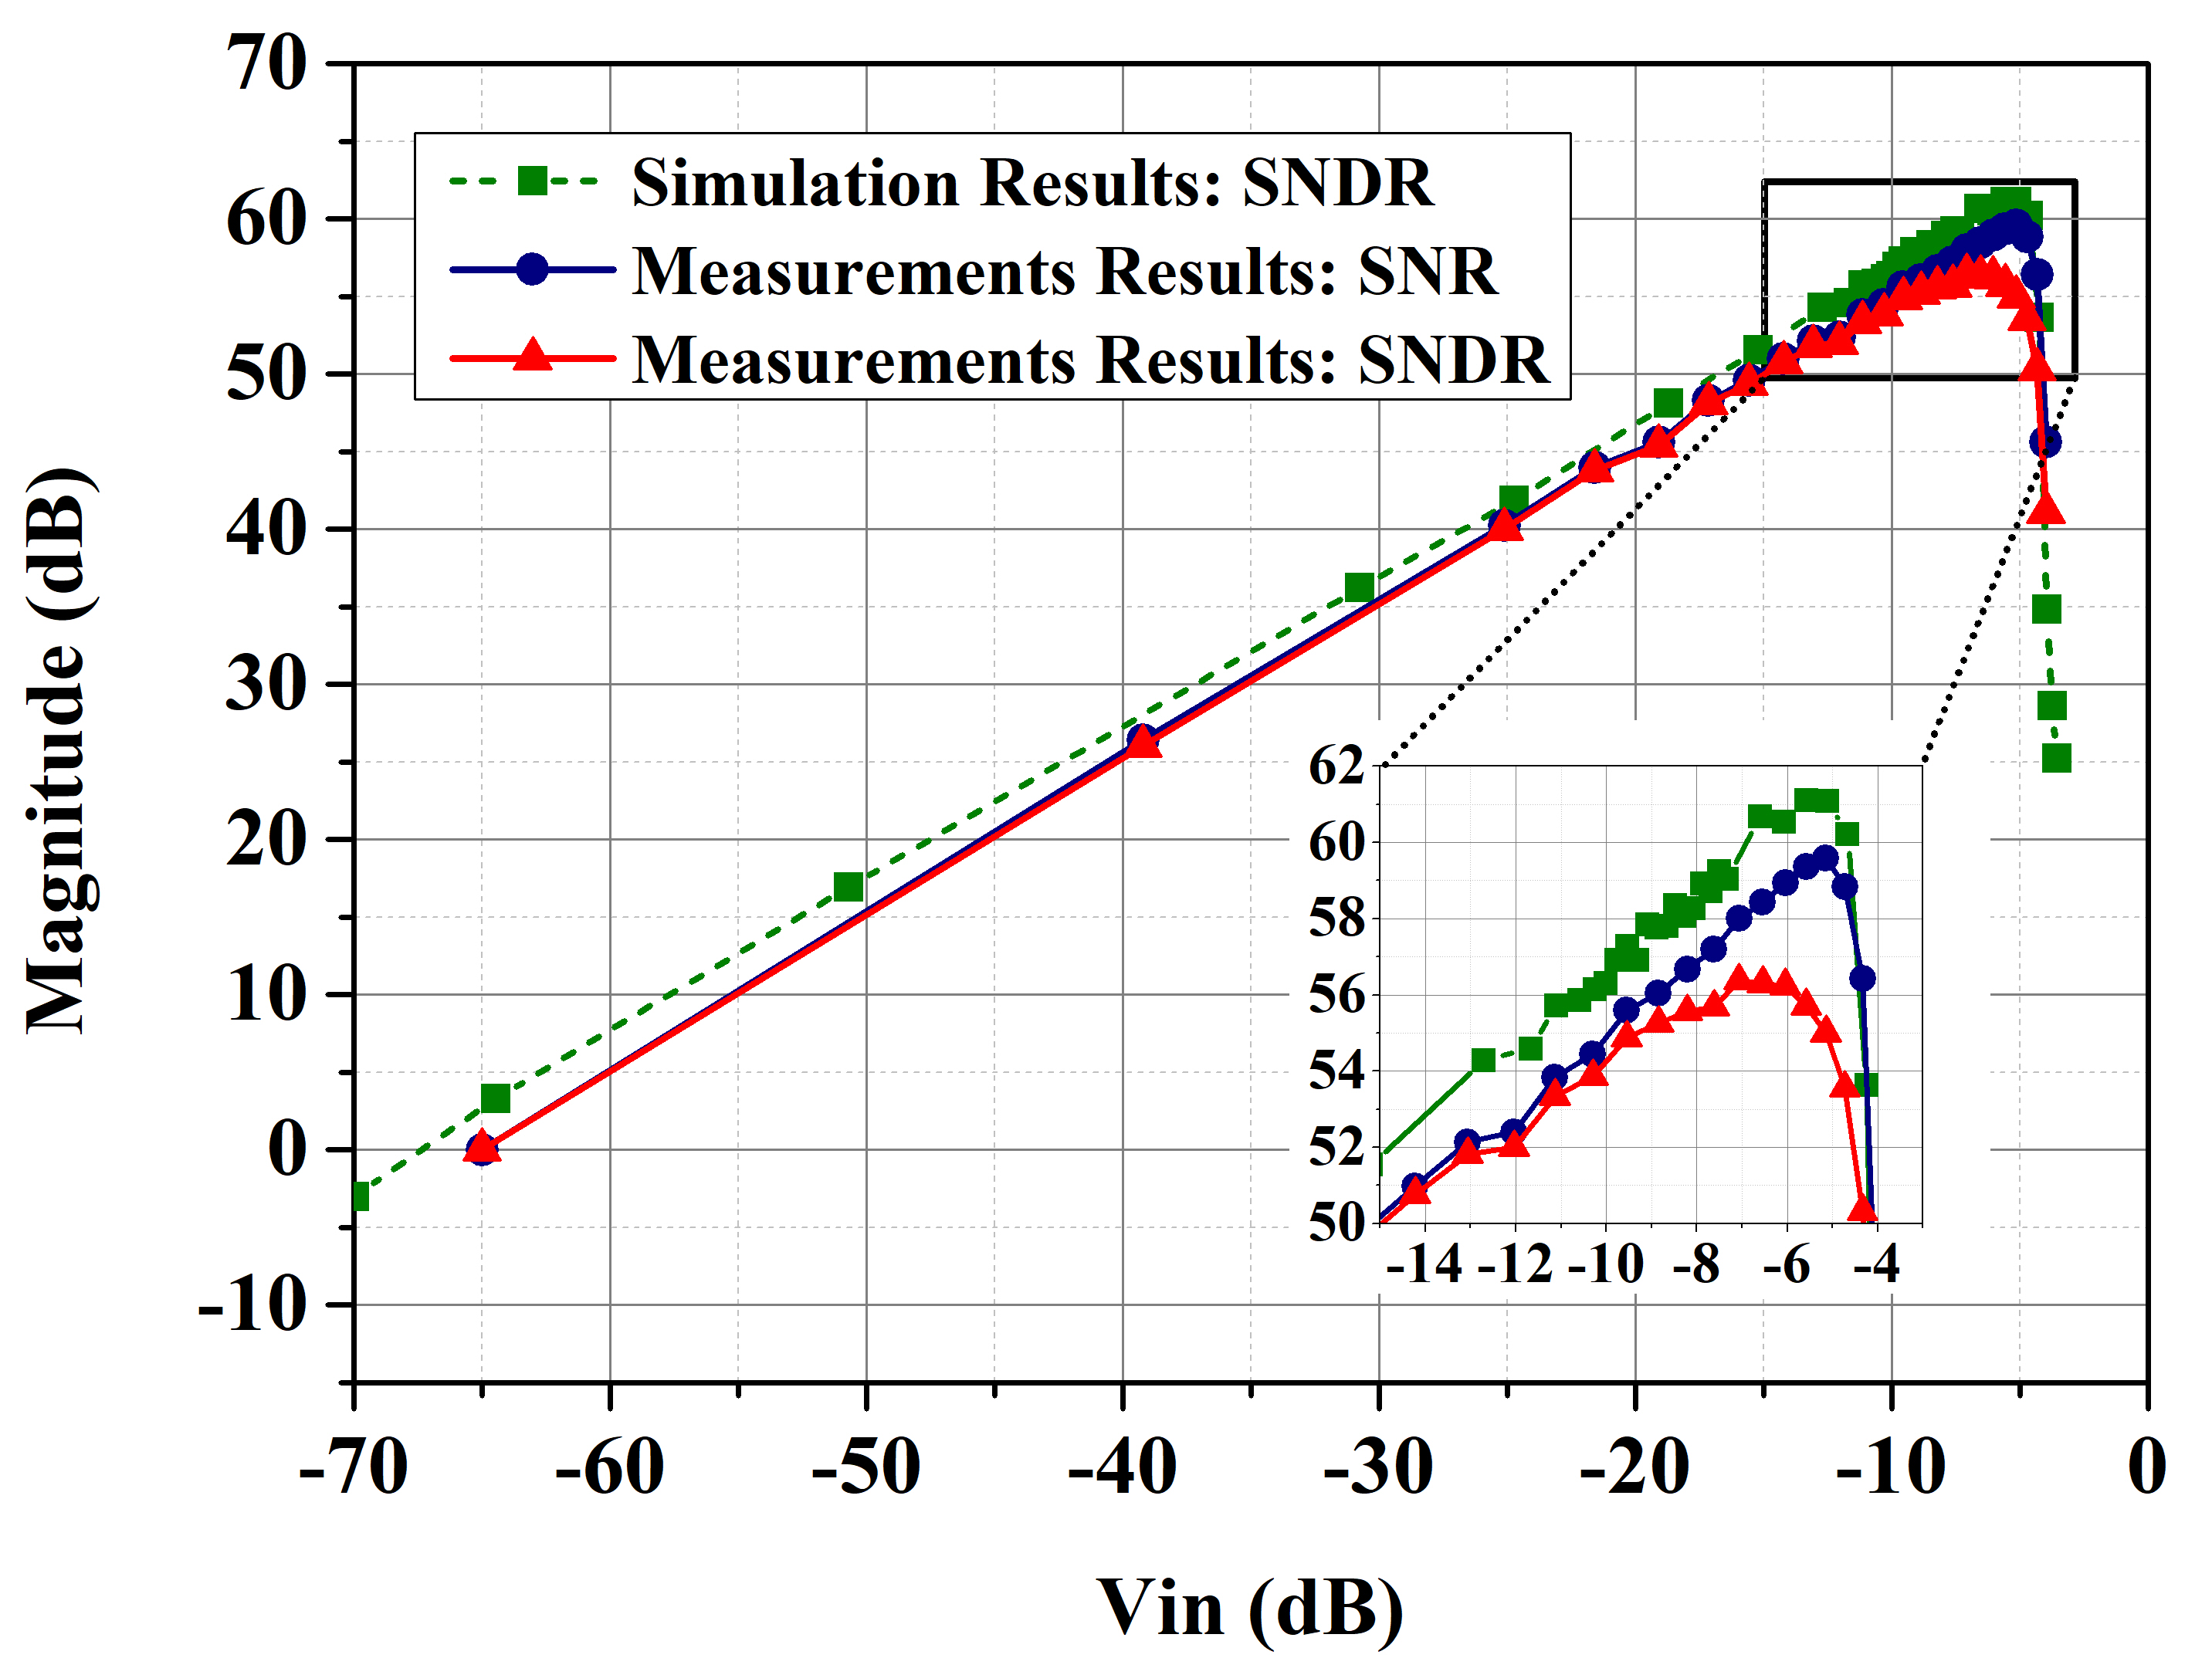
\includegraphics[width=0.8\columnwidth]{Chap06/Figures/snr_vs_vin.jpg}
    \caption{Performance of IADC as a function of input signal amplitude }
    \label{fig:iadc_snr_vs_input}
\end{figure}
%

The input signal is applied at a frequency of 100~kHz with an amplitude of -5~dB while the architecture is clocked at 80~MHz. The SNDR achieved with this setup is 55.0~dB, SNR of 59.58~dB and the DR is around 65 dB with noise floor residing at around -100~dB. The SNDR, SNR and DR are then measured as a function of the input signal amplitude and are plotted in Fig. \ref{fig:iadc_snr_vs_input}. From the graph it is clear that the maximum SNR that can be obtained from the IADC architecture is 59.58~dB at an input signal amplitude of -5.0~dB w.r.t. the full scale which makes it an MSA. In the subplot of the Fig. \ref{fig:iadc_snr_vs_input}, it can be seen that, as input amplitude is increased from -15.0~dB to -5.0~dB (an MSA), the SNR characteristic continues to raise linearly but SNDR diverges starts shifting down progressively as a consequence of harmonic distortion. The maximum SNDR that can be obtained is 56.37~dB and corresponding SNR is 58.0~dB at an input amplitude of around -7.0~dB. 

%
\begin{figure}[h!]
    \centering
    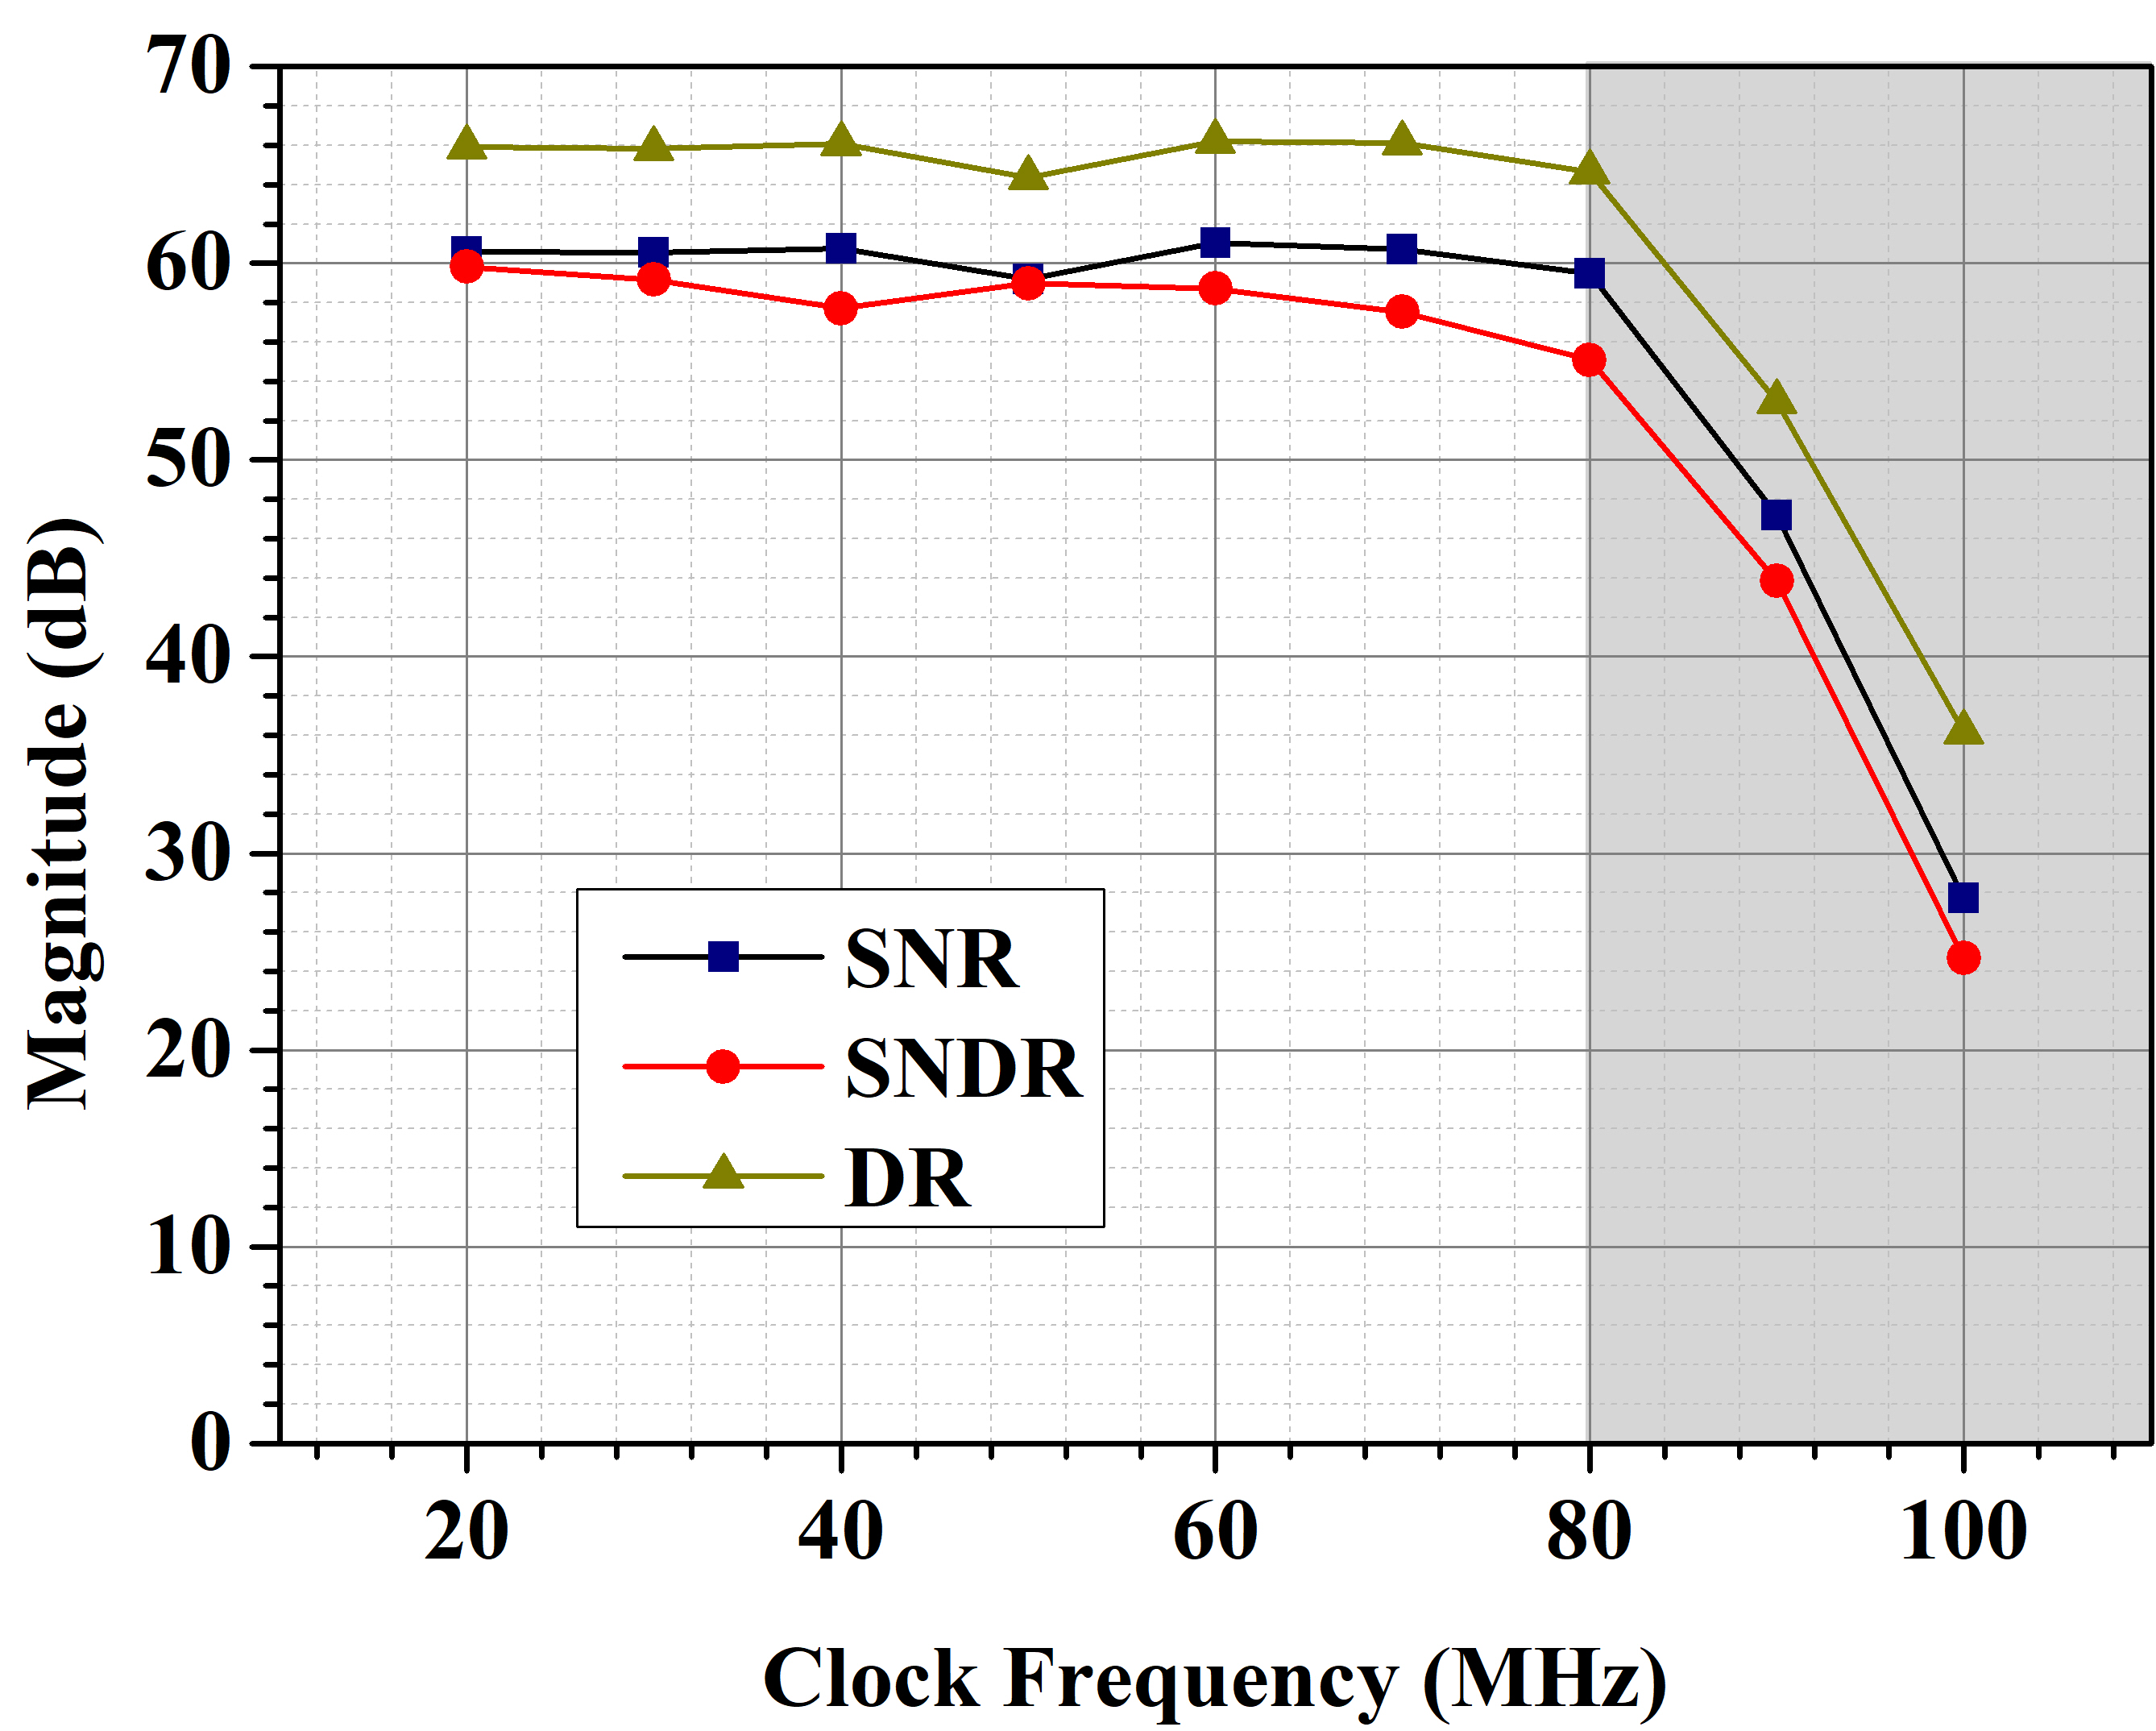
\includegraphics[width=0.8\columnwidth]{Chap06/Figures/snr_vs_fck.jpg}
    \caption{Performance of IADC as a function of clock frequency }
    \label{fig:iadc_snr_vs_clk}
\end{figure}
%

The architecture has been designed to work in an incremental mode at a maximum speed of 80~MHz. Therefore the performance of the structure for the clock frequency is verified by varying the clock frequency from 20~MHz to 100~MHz and the parameters are plotted as shown in Fig. \ref{fig:iadc_snr_vs_clk}. SNDR, SNR and DR stays almost constant for the clock frequencies from 20~MHz to 80~MHz but later on the performance degrades significantly when running it at 90~MHz and 100~MHz.

%
\begin{figure}[h!]
    \centering
    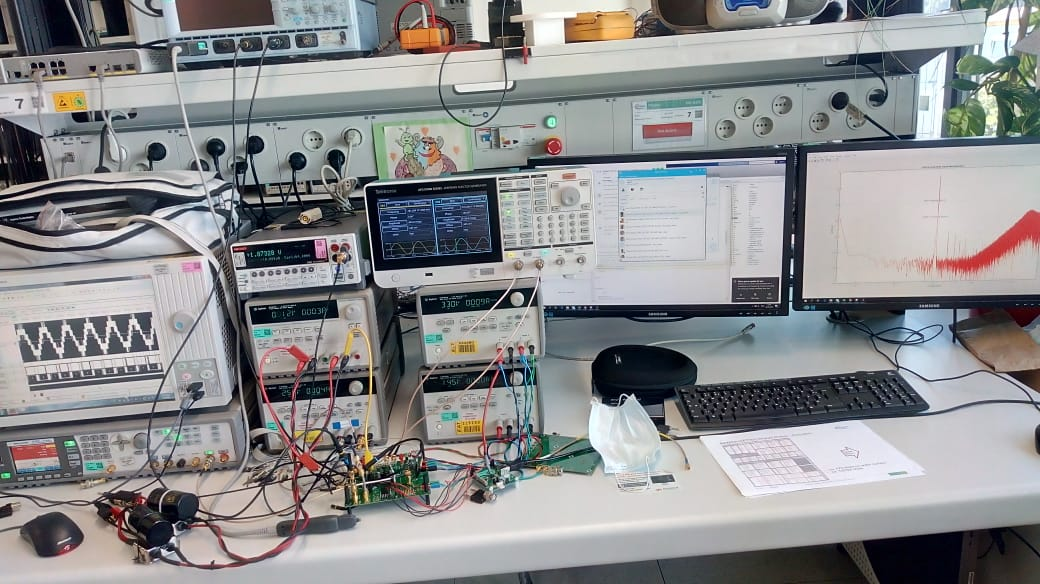
\includegraphics[width=\columnwidth]{Chap06/Figures/lab_setup.jpeg}
    \caption{A complete Set-up in the lab for the characterization of the samples}
    \label{fig:char_setup}
\end{figure}
%

\begin{table*}
    \centering
    \resizebox{\columnwidth}{!}{
    \begin{tabular}{l|cc|c|c|c|c|c|c}
        \Xhline{8\arrayrulewidth}
        Parameter    & \multicolumn{3}{c|}{\textbf{This Work}}                & \cite{ISSCC_FUKAZAWA}  & \cite{ISSCC_KIM}  & \cite{ISSCC_TURCOTTE}  & \cite{ISSCL_KATAYAMA} & \cite{TCAS1_VOGELMANN}\\ \hline
        Architecture & \multicolumn{2}{c|}{\textbf{SD-Mode}} & \textbf{I-Mode} & CT-MASH {\textSigma}{\textDelta} ADC   & CT-{\textSigma}{\textDelta} ADC  &  DT-MASH {\textSigma}{\textDelta} ADC  & IADC+Cyclic & Time-Interleaved IADC\\ \hline
        Technology      & \multicolumn{2}{c|}{\textbf{130 nm}}    & \textbf{130 nm}    & 28 nm & 65 nm & 130 nm & 180 nm & 180 nm\\ \hline
        Supply Current  & \multicolumn{2}{c|}{\textbf{2.6 mA}}     & \textbf{2.6 mA}     & 17 mA (A)+ 18 mA (D) & ---  & --- & ---  & 450 {\textmu}A \\ \hline
        Supply Voltage  & \multicolumn{2}{c|}{\textbf{2.5 V}}    & \textbf{2.5 V}    & 1.1 V(A)/1.0(D)/1.8  & 0.8 V & ---  & --- & 3 V \\ \hline
       Conversion Time & \multicolumn{2}{c|}{---} & \textbf{237.5 ns} & 250 {\textmu}s   & 1 ms & 50 {\textmu}s  & 800 ns  & 5 {\textmu}s \\ \hline
        Bandwidth  & 2.1 MHz  & \textbf{1.25 MHz}  & \textbf{2.1 MHz}    & 15 MHz   & 500 Hz  & 10 kHz & 625 kHz & 100 kHz \\ \hline
        $\mathit{SNR}_{\mathit{max}}$       & 66.4 dB  & \textbf{73.2 dB} & \textbf{59.6 dB} & 67.5 dB  & 66.2 dB  & 60.8 dB & 96.6 dB & 101.5 dB \\ \hline
        $\mathit{SNDR}_{\mathit{max}}$      & 63.0 dB & \textbf{63.0 dB}  & \textbf{56.4 dB}  & 67.5 dB  & 66.2 dB  & 60.8 dB & 96.6 dB & 101.5 dB \\ \hline
        $\mathit{FoM}$             & 151.5 dB & \textbf{156.0 dB} & \textbf{144.7 dB} & 156.5 dB & 154.1 dB  & 154.4 dB & 170.1 dB  & 163.8 dB\\\Xhline{8\arrayrulewidth}
    \end{tabular}
    }
    \caption{Performance summary of the proposed ADC and comparison with the state-of-the-art}
    \label{tab:comparison_table}
\end{table*}

The performances of the prototype ADC, for both SD-mode and I-mode, are summarized and compared with the state-of-the-art in Tab.~\ref{tab:comparison_table}. In order to have a fair platform for the comparison between different architectures, we used the Schreier figure of merit \cite{IEEEPRESS_SHREIER}, defined in Eq. \ref{eq:FoM}

\begin{equation}\label{eq:FoM}
    \mathit{FoM} = \mathit{SNR}_{\mathit{max}}+10\log_{10}\left({\frac{\mathit{Bandwidth}}{\mathit{Power}}}\right).
\end{equation}

% \begin{figure}[h]
%     \centering
%     \subfigure[]
%     {
%         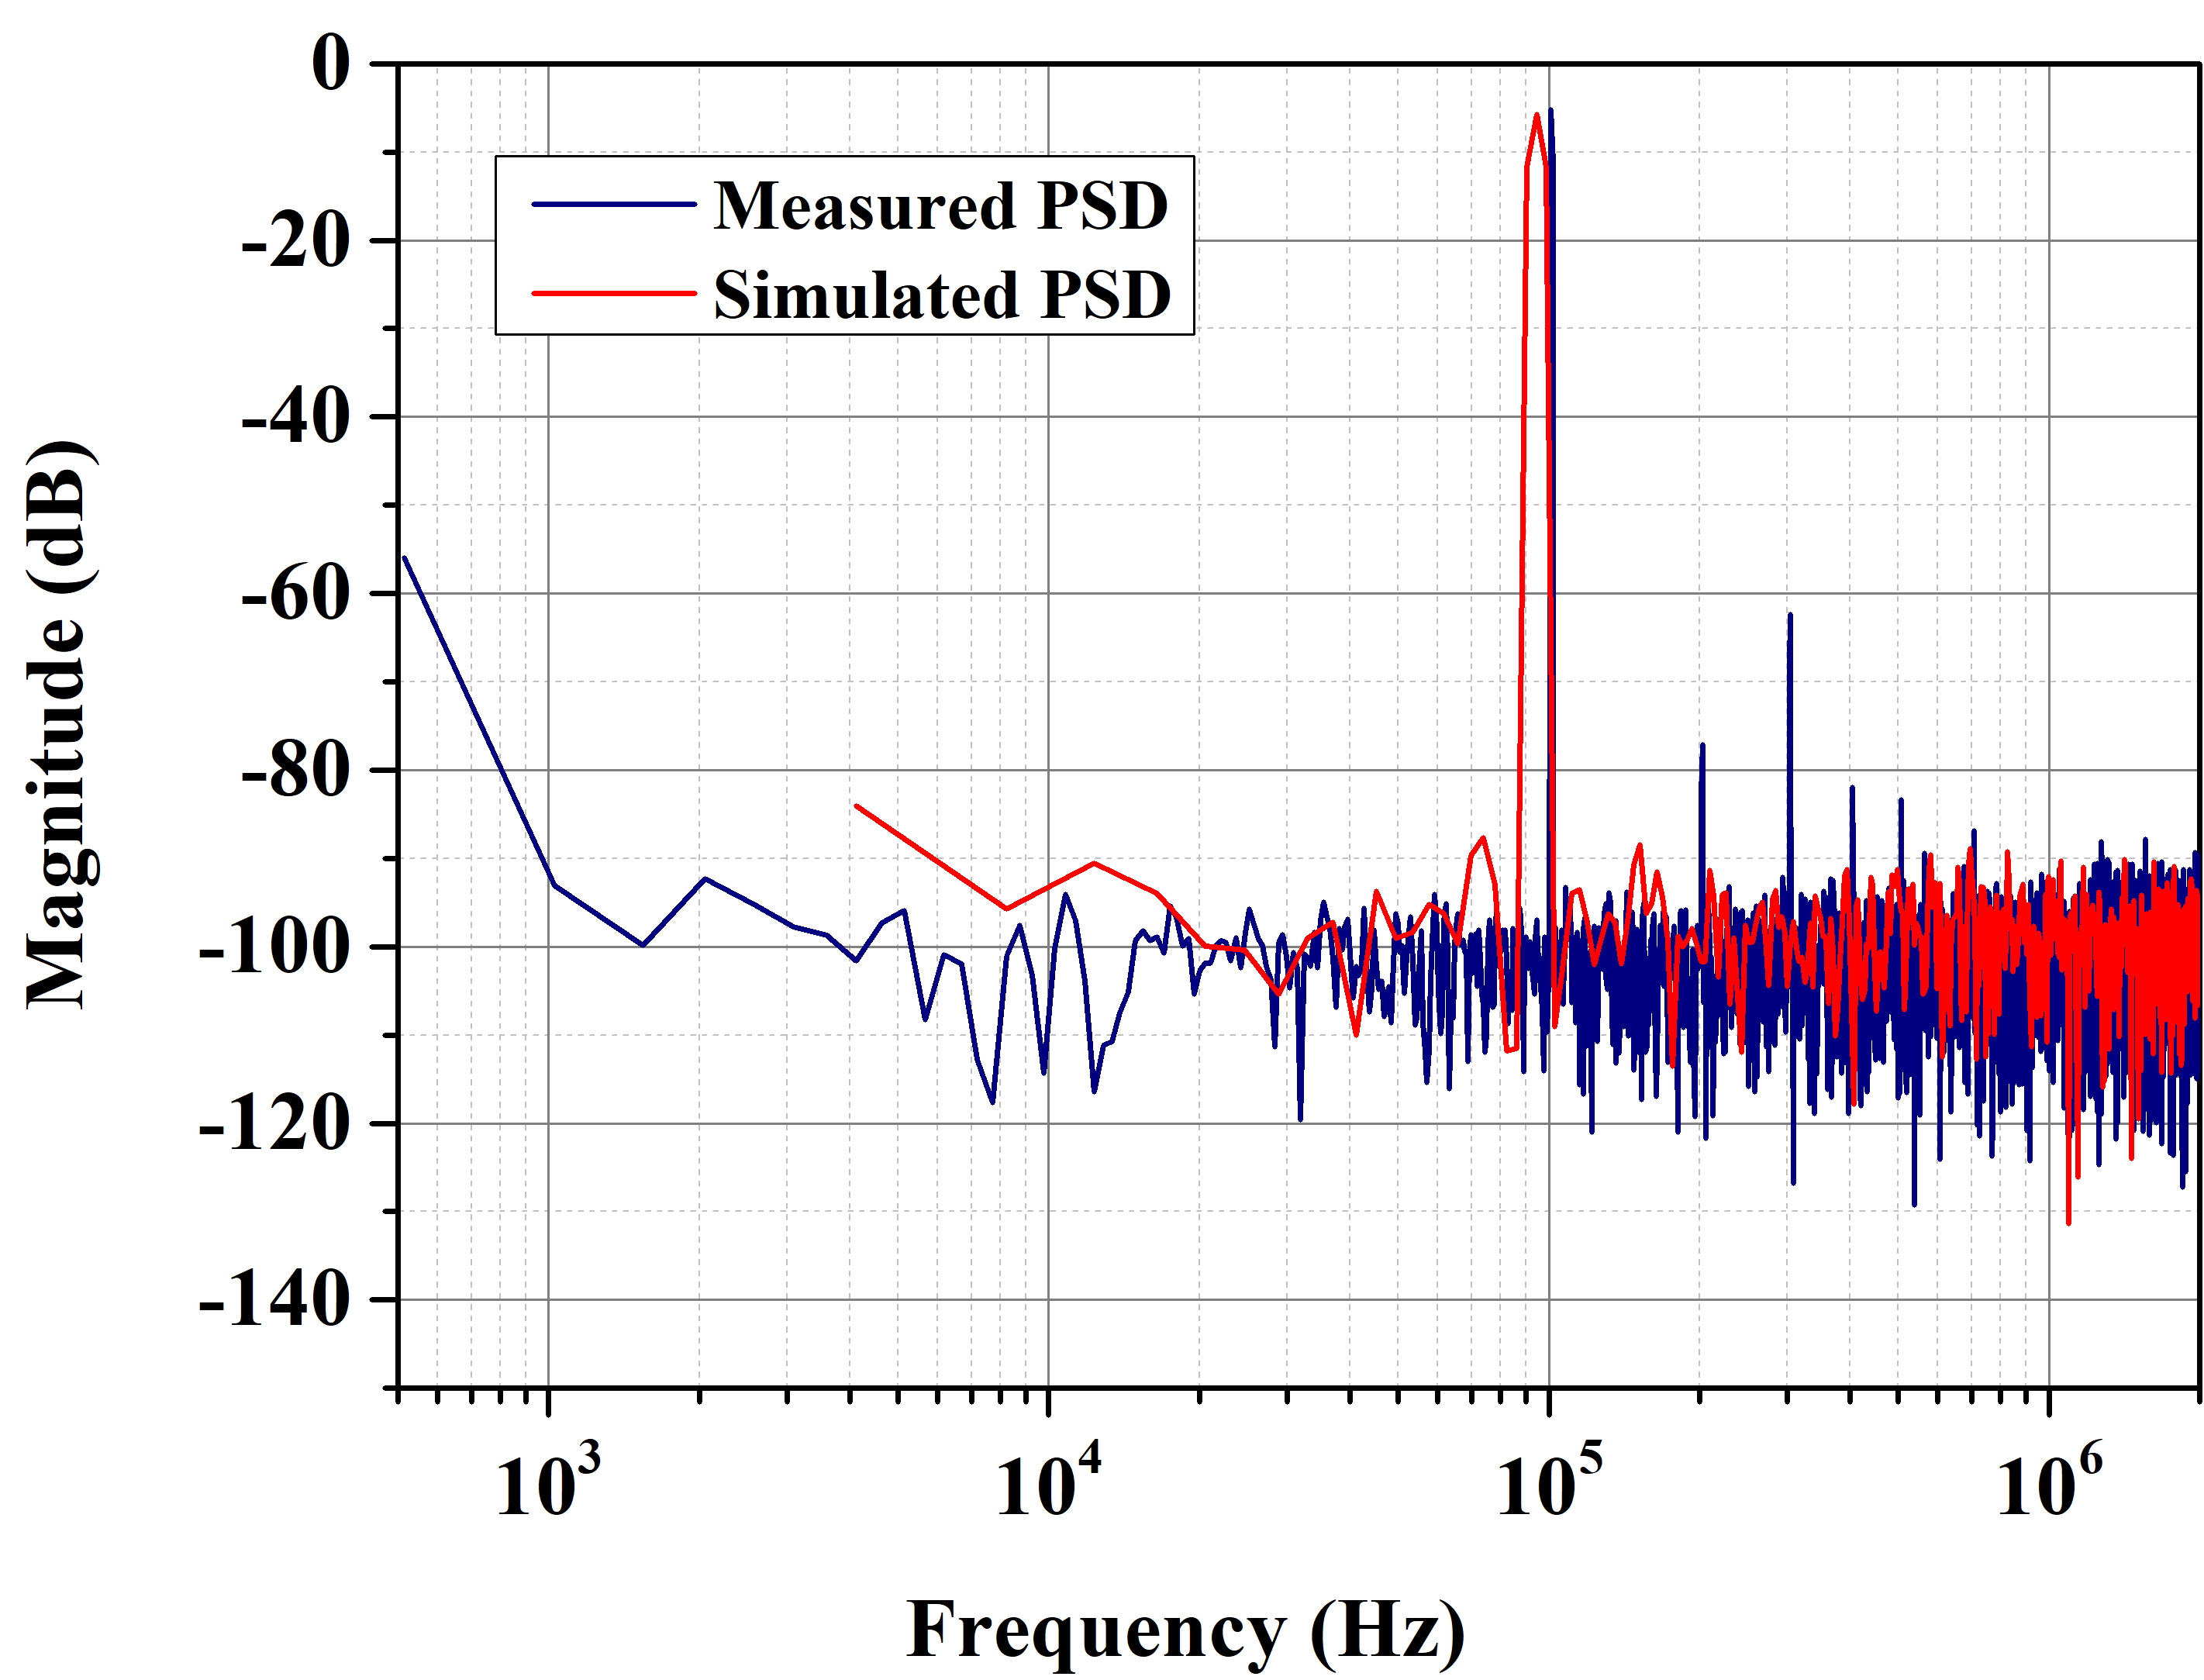
\includegraphics[scale=.28]{Chap06/Figures/PSD_IADC_sim_meas.jpg}
%     }
%     \\
%     \subfigure[]
%     {
%         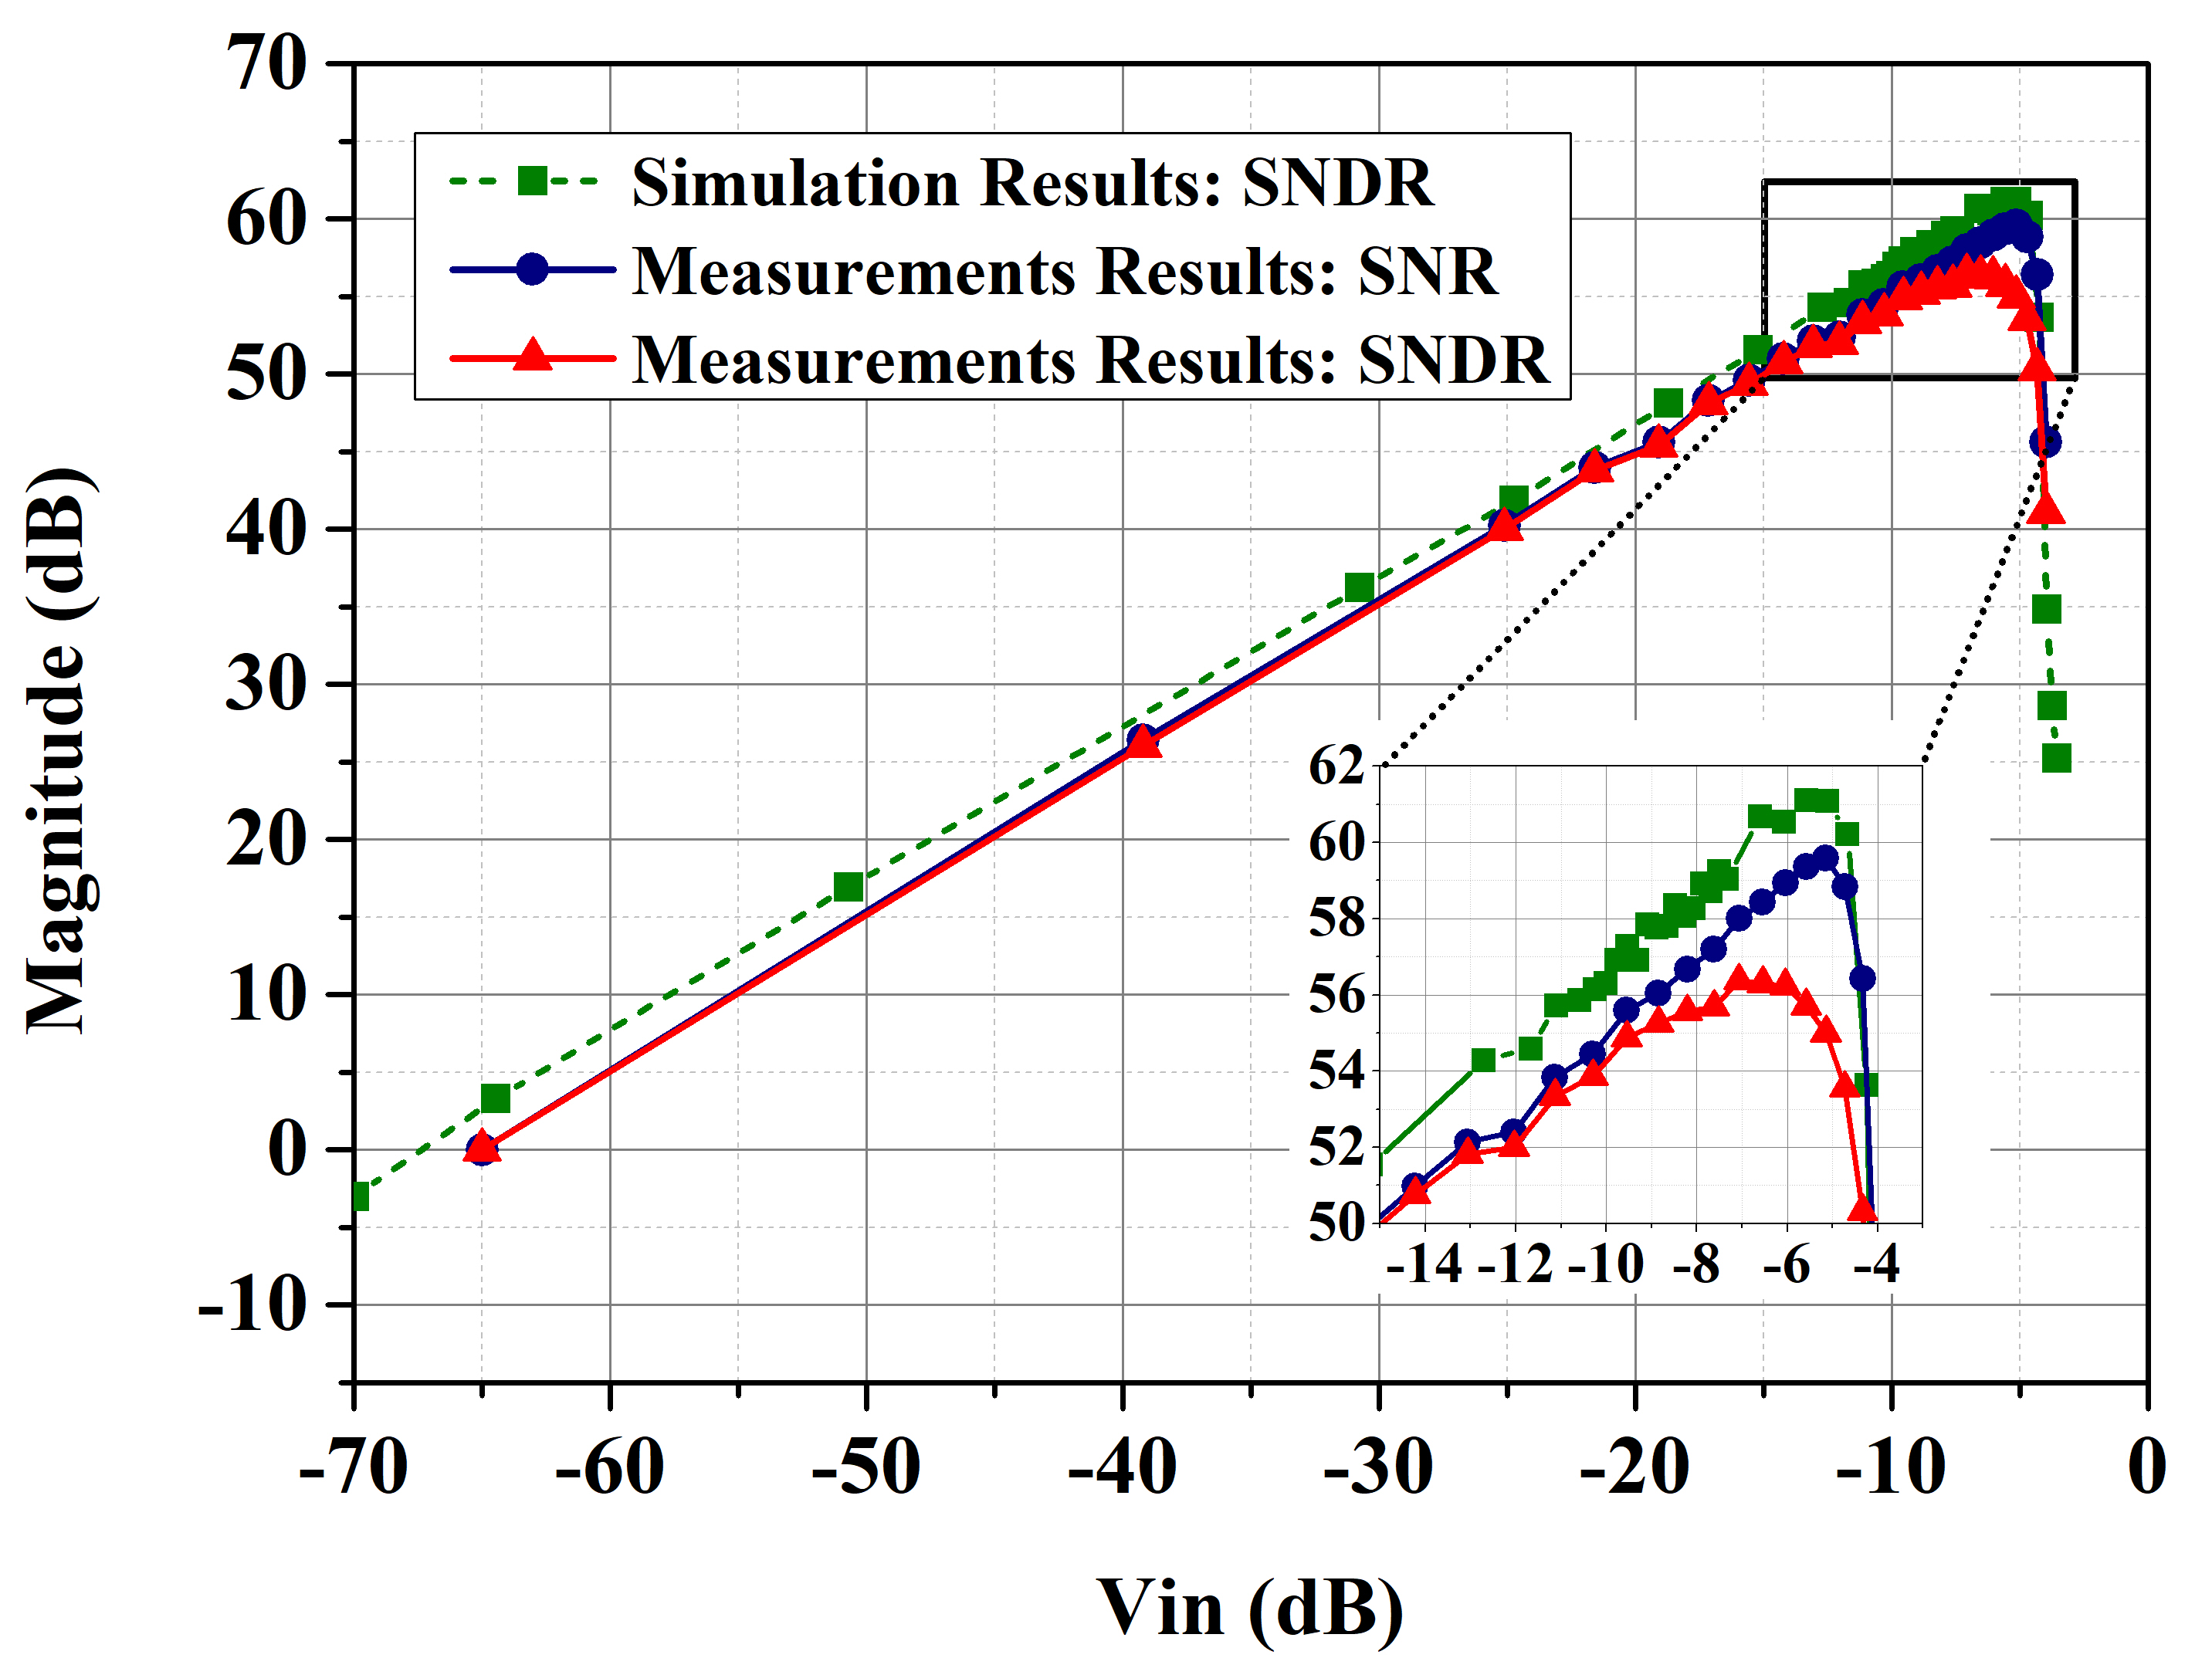
\includegraphics[scale=.28]{Chap06/Figures/snr_vs_vin.jpg}
%     }
%     \qquad
%     \subfigure[]
%     {
%         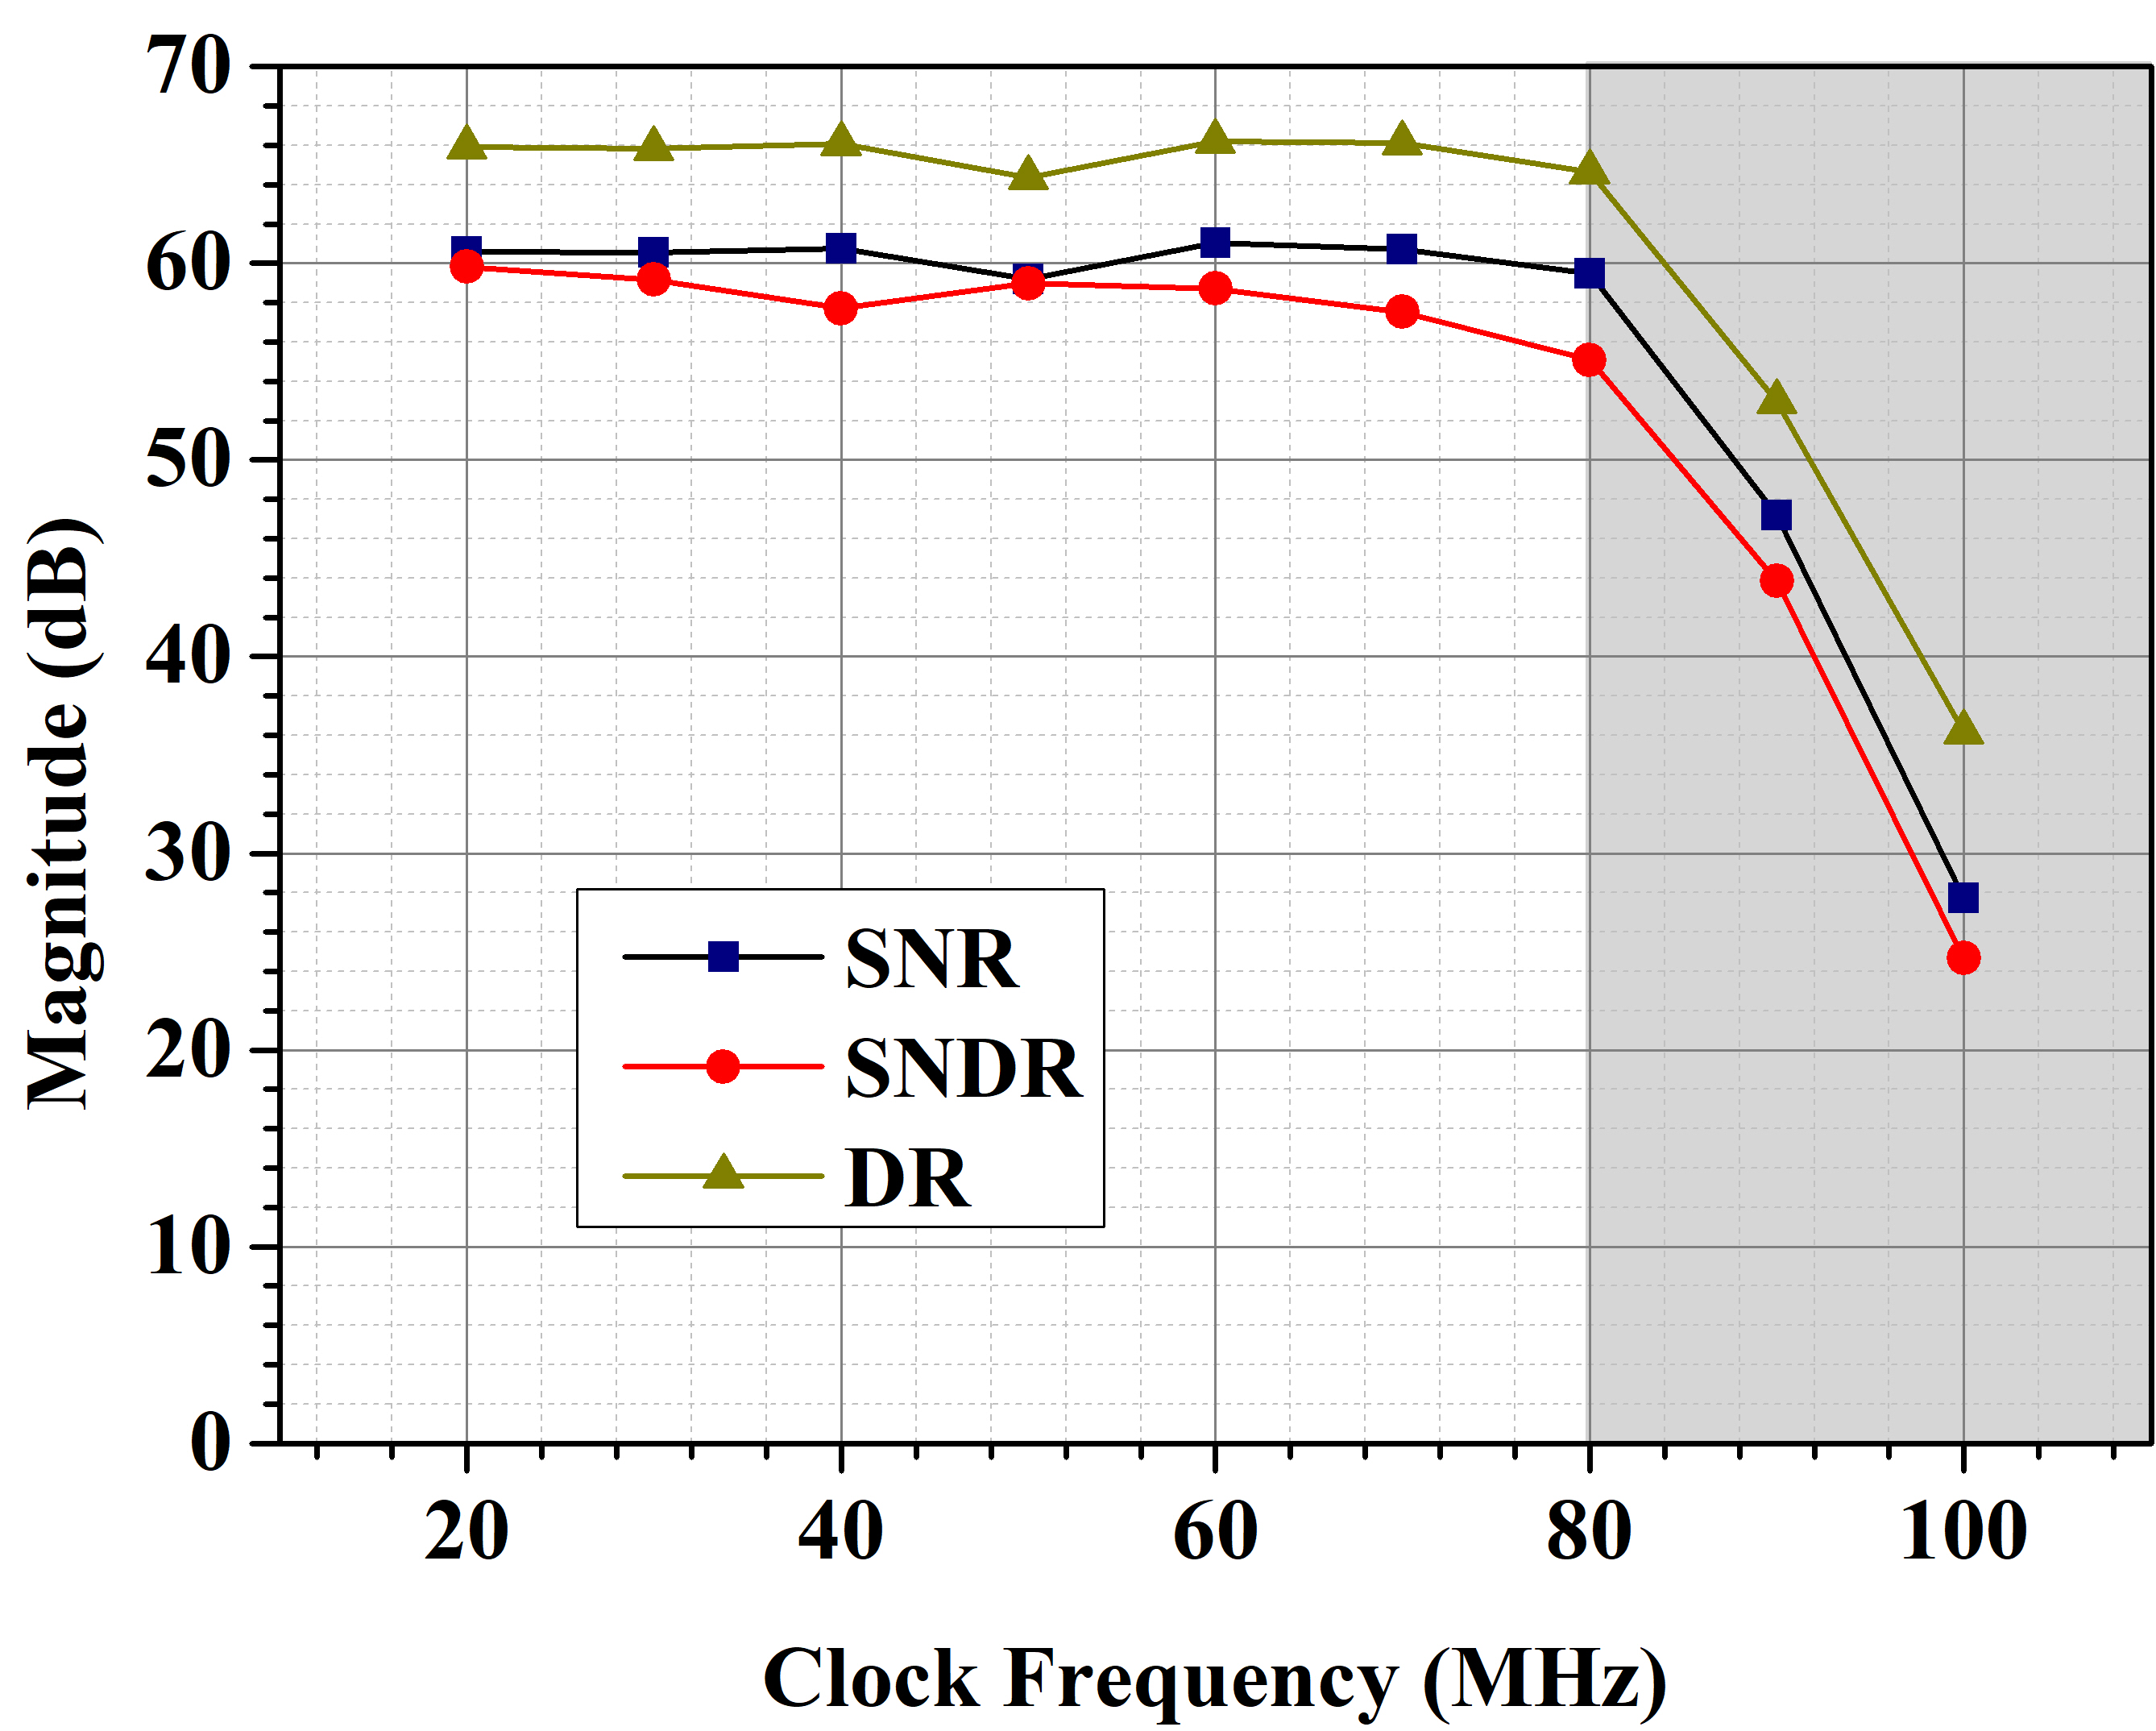
\includegraphics[scale=.28]{Chap06/Figures/snr_vs_fck.jpg}
%     }
%     \caption
%     {
%         (a) PSD of the Incremental ADC
%         (b) Performance of IADC as a function of input signal amplitude
%         (c) Performance of IADC as a function of clock frequency
%     }
%     \label{IADC_meas}
% \end{figure}